\documentclass[degree=master,bibtype=numeric]{tongjithesis}
% 选项:
%   degree=[master|doctor], 							% 必选
%   bibtype=[numeric|authoryear], 						% 可选,数字式引用|作者-年份引用,默认为数字式(上标)引用
%   degreetype=[academic|profession|equaleducation],  	% 可选, 学术型|专业型|同等学力,默认为学术型
% 	electronic,                                 		% 可选, 电子版,(打印时删除)
%   secret,                                     		% 可选,是否保密,基本不用
%   pifootnote,                                 		% 可选,默认已打开
%   romantitle                                  		% 可选,默认已打开
%   注:默认已打开的选项可以使用arialtitle=false的形式关闭。

% 所有其它可能用到的包都统一放到这里了,可以根据自己的实际添加或者删除。
\usepackage{tongjiutils}
\usepackage{listings}
\usepackage{xcolor}
\usepackage{colortbl}
\usepackage{algorithm}
\usepackage{algorithmic}
\usepackage{bm}
\usepackage{booktabs}
\usepackage{graphicx}
\usepackage[graphicx]{realboxes}
\usepackage{longtable}
%参考文献更新使用biblatex包, 使用gb7714-2015标准, 具体参数设置可在cls文件中搜索biblatex进行了解
%加入bib文件(老版本文件依然能够使用)
\addbibresource{ref/refs.bib}   

\begin{document}

% 定义所有的eps文件在 figures 子目录下
\graphicspath{{figures/}}


%% 封面部分
\frontmatter
\tongjisetup{
  %******************************
  % 注意:
  %   1. 配置里面不要出现空行
  %   2. 不需要的配置信息可以删除
  %******************************
  %
  %=====
  % 秘级
  %=====
  secretlevel={保密},
  secretyear={2},
  %
  %=========
  % 中文信息
  %=========
  % 题目过长可以换行。
  ctitle={面向无人机自主堆体体积测量的视觉定位及重建方法研究},
  cheadingtitle={面向无人机自主堆体体积测量的视觉定位及重建方法研究},    %用于页眉的标题,不要换行
  cauthor={何士波},  
  studentnumber={1732940},
  cmajorfirst={工学},
  cmajorsecond={控制工程},
  cdepartment={电子与信息工程学院},
  csupervisor={岳继光~教授}, 
  % 如果没有副指导老师或者校外指导老师,把{}中内容留空即可,或者直接注释掉。
  cassosupervisor={董延超~副教授}, % 副指导老师
  % 日期自动使用当前时间,若需指定按如下方式修改:
  % cdate={超新星纪元},
  % 没有基金的话就注释掉吧。
  %cfunds={(国家杰出青年基金 (No.123456789) 支持)},
  %
  %=========
  % 英文信息
  %=========
  etitle={Visual localization and reconstruction method for autonomous bulk measurement of unmanned aerial vehicle}, 
  eauthor={He ShiBo},
  emajorfirst={Engineering},
  emajorsecond={Control Engineering},
  edepartment={College of Electronics and Information Engineering},
  %efunds={(Supported by the Natural Science Foundation of China for\\ Distinguished Young Scholars, Grant No.123456789)},    
  esupervisor={Prof. Yue Jiguang},
  eassosupervisor={V.P. Dong Yanchao}
  }

% 定义中英文摘要和关键字
\begin{cabstract}  
  在现代工业中,随着工业生产水平的提高,为了加强对堆体物料库存量的监控,针对堆体积测量的需求也逐步提升。传统测量方案一般都是选用激光雷达,测重地磅等复杂仪器来完成测量工作,这些仪器可以一定程度的完成测量工作并获取测量真实值。但依旧存在很多问题限制以上测量技术在行业内的广泛应用,例如测量仪器成本过高,安装复杂,单一场景内的仪器难以复用;测量过程需要人力参与,难以实现全自动化的测量流程;测量精度年久失衡,难以保证测量精度。针对以上情况,本文提出了一种在封闭电厂环境下,通过无人机的自主定位和飞行,对煤堆体进行图像采集工作,随后根据采集的图像进行三维重建得到高精度堆体点云模型,对点云模型估计体积值以获取堆体体积的完整测量流程。本文所提出方案完全基于计算机视觉实现,成本可控,且能在各种场景中复用。
  
  针对无人机的自主定位和飞行方法研究。本文提出在封闭无GPS的环境中,使用纯视觉的方式来完成无人机的自主定位和飞行工作。通过在场景中放置二维码,来解决视觉SLAM无法确定尺度的问题,并且结合SLAM坐标系和二维码坐标系对无人机提供真实世界坐标系下的位姿信息。
  
  针对连续图像的高精度堆体三维重建方法研究。本文提出一种结合SLAM结果的堆体三维重建方法,以有序图像作为SLAM输入,关键帧数据集作为输出提供给三维重建系统以获取高精度点云。解决传统三维重建图像匹配耗时,点云精度低的问题。
  
  针对堆体点云进行体积估计方法研究。本文提出一种基于计算机视觉方案的堆体体积估计方法,依次对生成的点云进行滤波获取高精度点云,估计三维点云的实际尺度,确定点云模型水平面等工作,最后根据纯点云信息估算场景中堆体的体积大小。
  
  基于真实环境下,对堆体体积测量进行分模块测试。实验结果表明,无人机的定位误差在高度方向可以控制在0.2m以内,整体定位精度在5$\%$以内,该精度完全可以提供给无人机循迹使用;改进后的三维重建模块则能加快匹配流程,获取较高精度的堆体三维点云,以满足体积测量的需求;最后的体积测量模块,可以估计出准确的尺度大小和水平面解析方程,通过对点云体积的求解获得堆体体积,测量误差可以控制在2$\%$以内。
\end{cabstract}

\ckeywords{立体视觉,SLAM,无人机定位, 三维重建,体积测量}

\begin{eabstract}
abstract
\end{eabstract}

\ekeywords{keywords}
\makecover


% 目录
\tableofcontents
% 符号对照表
%\begin{denotation}
%\item[GNU] GNU's Not Unix /'gnu:/
\item[GFDL] GNU Free Documentation License
\item[GPL] GNU General Public License
\item[FSF] Free Software Foundation
\item[SMP] 对称多处理
\item[API] 应用程序编程接口
\item[$E$] 能量
\item[$m$] 质量
\item[$c$] 光速
\item[$P$] 概率
\item[$T$] 时间
\item[$v$] 速度

%\end{denotation}

%%% 以下索引按需要选择
% 插图索引
\listoffigures
% % 表格索引
% \listoftables
% % 公式索引
% \listofequations
%%% 正文 
\mainmatter
% \chapter{绪论}
\label{cha:chap1}
\section{研究背景和研究意义}
\label{sec:1.1}
\subsection{研究背景}
\label{sec:1.1.1}
人类通过双眼来探索与发现世界,在接收外部信息的方式中,有不到三成来自于听觉、触觉、嗅觉等感受器官,而超过七成、最丰富、最复杂
的信息则通过视觉进行感知的。计算机视觉便是一种探索给计算机装备眼睛(摄像头)与大脑(算法)的技术,以使计算机能够自主独立的控
制行为、解决问题,同时感知、理解、分析外部环境。

20世纪60年代,计算机视觉得到了最初的发展,该阶段的研究重心主要体现在如何从二维图像中恢复出如立方体、圆柱体等立体化的三维形
状,解释各个物体的空间位置关系。1982年David Marr从信息处理的角度对数学、神经生理学、计算机图形学等学科的研究成果进行了归纳
总结,并在此基础上提出了一系列计算机视觉理论,经典Marr视觉信息处理过程如图~\ref{fig:introduction_Marr}所示。得益于这个完
整明确的理论体系,计算机视觉得到了蓬勃的发展,它的核心思想是从二维图像恢复三维结构。
\begin{figure}[H] % use float package if you want it here
  \centering
  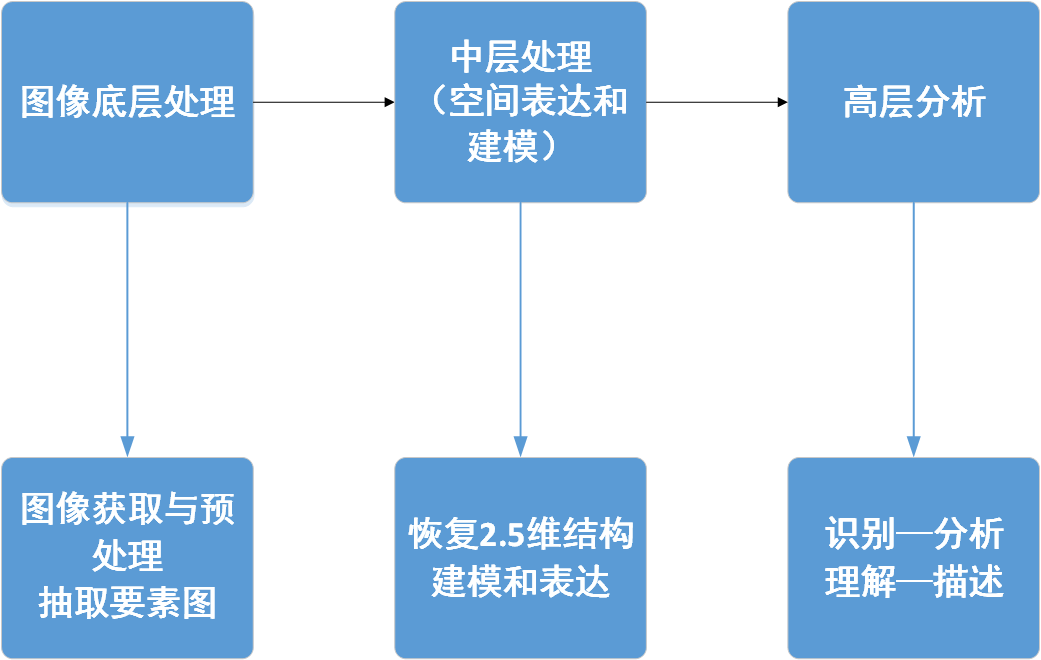
\includegraphics[height=6cm]{introduction_Marr.png}
  \caption{经典Marr视觉信息处理过程示意图}
  \label{fig:introduction_Marr}
\end{figure}
近年来,图像的三维重建在计算机视觉中发挥了很大的作用,并且在质量和性能上有了较大的提升。其主要应用是自动地对于难以建模的对象
建模,加快了图像运用的建模过程。这种技术需要处理大量的数据,可以使用于室内和室外的场景, 而不受控制的环境通常影响室外场景,如
密集建筑群,或者复杂的原始森林等。对于这些场景,虚拟现实和计算机模拟可以被用来分析工作环境和工作难度等方面,三维图像重建技术
本身被视为一个生成3D模型的技术。快速有效完整重建类似于雕塑三维物体目标的三维模型成为目前的研究方向。由连续图像的三维重建主要
是指从二维图像序列中的获取物体的信息并进行三维重建。然而,这个领域并没有引起人们足够的重视,因此本文将对三维重建的具体原理以及
改善展开讨论。

当前在一些工业场景中,需要对其中场景进行测量,主要包括场景的高度,面积,体积,甚至于温度,湿度分布等,传统方式中主要采用雷
达扫描场景的方式来进行,但考虑到该雷达本身成本较高,受场景的限制也很大,在室外环境或者大尺度环境下,就难以发挥作用。现在更多
采用计算机视觉的方式来解决这些问题,可以根据三维重建的点云结果测量以上所描述的几何特性,这样做只需要结合摄像机和测量算法即
可实现,可以很简易的复现在多种场合中。
\subsection{研究意义}
\label{sec:1.1.2}
本文的研究目标是让无人机能够在全封闭或者半封闭的环境中,完全基于视觉的方法完成自主飞行任务,并且在飞行的过程中,采集待测物
体的实拍图像,进行三维重建,最终根据三维重建的点云结果测算待测物体的体积值。

传统无人机的飞行都需要依靠操作员手动控制,或者是基于GPS定位结果进行巡航,本文提出了一种完全基于纯视觉的方法来进行无人机定位
的导航得到的方法,该方法可以在全封闭无GPS的环境中,为无人机提供定位信息,解决了场景限制的问题,并且整个无人机的飞行过程可以
完全自动化的运行,并对场景进行图像采集。

从二维图像重建三维立体具有重要的研究价值和潜在经济社会价值,其核心技术是通过运动来恢复结构。三维重建系统在不同的应用领域有
着不同的预设条件和技术要求,主要包括医学领域的重建系统,机器人导航相关实时重建系统,工业领域包括3D打印在内的室内高精度重建
系统,以及摄影测量领域实景三维重建系统。 三维重建已能提供完整方案,但传统三维重建算法得到的点云结果存在精确度不高,场景无
法闭合等问题,本文提出一种结合SLAM结果的三维重建方法,拟生成一个高精度,强鲁棒的点云地图。

有关实景物体三维测量,传统方法常采用激光雷达,声波等方案,这些方案成本较高,且对场景有限制要求要求,本文提出了一种基于三维
重建后的点云结果进行体积估计的方法,可以极大降低成本且能够在多重场合下复用算法。

因此基于无人机自主飞行采集图像数据的三维重建和体积测量有着十分重要的工程意义,并且在很多场合下,整体流程可靠性和可行性都得
到充分验证。


\section{国内外研究现状}
\label{sec:1.2}
本文主要涉及到的理论方法有及时定位与地图构建(Simultaneous localization and mapping,简称SLAM),三维场景重建,
视觉体积测量等几个方面对国内外研究现状和发展动态进行描述。
\subsection{SLAM的研究现状}
\label{sec:1.2.1}
SLAM(即时建图与定位)是一种在定位导航的同时,进行构图的技术\cite{cadena2016past}。最早的SLAM技术还不是使用视觉的方法,
而是使用声波传感器或者激光以及惯性测量单元实现环境建模和自身定位,直到21世纪,Stephen Se等人首次使用图像的特征点实现视觉
SLAM\cite{se2002mobile},之后由$Davison$使用$EKF$框架实现了最早的单目实时SLAM系统\cite{davison2003real},奠定了单目系统
的基础;Davison在2007年成功实现基于单相机的纯视觉SLAM系统,算法的关键是在线建立2D点到3D点的映射关系,并且使用实时运动模
型估计相机的位置\cite{davison2007monoslam};Mur-Artal使用ORB特征点作为地图构建特征点,大幅度降低了点云的数量,并且使用
回环检测的方法使定位与建图的精度都大幅提升\cite{mur2015orb};随着硬件计算能力和数据储存的提升,提取目标深度信息的技术得
到了很大的发展,戚传江等人使用2D slam的解决方案,采用多传感器数据融合的方法,完成多自由度位姿检测,拓展了SLAM的应用场
景;Whelan的实验通过使用体积融合的方法实现了实时大范围的稠密RGB-D的SLAM系统\cite{whelan2015real}。

Durrant-Whyte和Bailey首先对前20年里SLAM的发展做出了详细的历史回顾,
并提出了概率方法和数据融合\cite{Gibbens2000A,durrant2006simultaneous},Aulinas等人提出在SLAM中添加滤波方法减少噪音影响
\cite{cadena2016past},Grisetti等人就SLAM后端进行详细阐述\cite{grisetti2010tutorial},Dissanayake研究了SLAM的基本性质,
包括可观测性、收敛性和一致性等\cite{dissanayake2011review}。近几年来,SLAM的发展更多的开始和机器人领域相结合, 
Saeedi提出了多协同机器人SLAM解决方案\cite{saeedi2016multiple},Stachniss发布了在SLAM领域机器人开发
手册\cite{stachniss2016simultaneous}。

应用到目标跟踪领域,单纯点云集还是无法满足要求,因此需要将点云数据语义化,Reiger使用关系树的方法实现物体的语义识别
\cite{sarkar2012slam},这项技术对于目标跟踪是很重要的;之后Sarkar在Reiger的研究基础上结合FastSLAM的方法,使得识别速度
更快,鲁棒性更强;Zhang, G等人使用基于线条的SLAM算法\cite{zhang2015building}提高物体识别的准确率,该方法能够对物体的边
沿与轮廓进行稳定的识别。

当使用单目相机运行SLAM算法时,依旧还存在很多的挑战,ORB-SLAM2\cite{mur2017orb}和LDSO\cite{gao2018ldso}
可能是目前单目SLAM中最先进的方法。然而,这些方法还存在很多的局限性,无地图复用,无法纯旋转,场景需丰富等,
并且用于重定位的方法\cite{galvez2012bags}在视点变化、重复模式和随时间变化时的性能有限。另一种估计相机姿态的方法是使用放置
在环境中的人工标记,最近的SPM-SLAM\cite{munoz2019spm}解决了之前描述的一些限制,它使用二维码而不是自然特征,但是也存在场
景中摆放大量二维码的问题。UcoSLAM\cite{munoz2019ucoslam}则提出了一种结合自然点和人造二维码的SLAM运行方法。

\subsection{三维重建的研究现状}
\label{sec:1.2.2}
照相机/摄像机是将一个三维场景或物体投影到二维平面上,但是在降维的过程不可避免地会损失存在信息,而利用三维重建技术,就是从获
取到的二维图像中复原原始三维场景或物体,三维重建的结果如图~\ref{fig:3d_constr}所示。

\begin{figure}[H] % use float package if you want it here
    \centering
    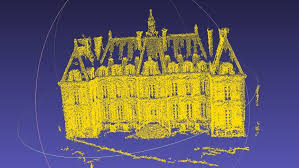
\includegraphics[height=8cm]{3d_constr.png}
    \caption{三维重建结果示意图}
    \label{fig:3d_constr}
  \end{figure}
CMU大学的Tomasi和Kanade\cite{tomasi1992shape}等人首先开发出了基于图片的三维重建系统,并利用仿射分解法对摄像机进行了标定,
得到摄像机运动参数,然后重构出物体的空间模型。随后,INRIAB Bougnoux等人\cite{bougnoux1997totalcalib,debevec1998image}
利用未标定的SfM和摄像机自标定等算法,开发了一个提升型三维重建模型。Berkeley大学的Debevoc\cite{beardsley19963d}等人完成了
著名的建筑物重构系统Façade,该系统要求首先得到建筑物的粗略几何模型和摄像机运动参数。Shum等人开发的人机交互式重构系统,利用
物体的一组全景图,即从各个角度得到物体的n张图片,然后对这些图像进行处理,重构出其三维实体,或者将场景表示成一系列按深度划分
的分层的集合。Faugeras等采用摄像机的自标定方法,利用分层重构等经典的方法,从图像序列中重构出建筑物的形貌。Katholieke大学
的Pollefeys等提出物体表面自动生成系统,该系统是在内参数可以改变的情况下,对摄像机采取了自标定的技术,该系统只要求用摄像机
绕物体周围一周,拍到一系列的图像,就可以自动实现自标定和分层重构。

\subsection{基于视觉体积测算的研究现状}
\label{sec:1.2.3}
基于
\subsection{语义结构化地图的研究现状}
\label{sec:1.2.4}
基于
\section{待解决问题}
\label{sec:1.3}
当前基于无人机自主飞行采集图像数据进行三维重建以及体积测量的方案还存在很多的待解决问题,如:\\
(1)	无人机在完全封闭环境中依靠纯视觉进行定位和建图,难以获取高精度的飞行位姿和地图信息。\\
(2)	基于三维重建算法对场景进行三维重建时,面临整个流程耗时长,输出点云噪音点大,需要对传统三维重建进行提升,以获取高精度
强鲁棒性的大尺度地图。\\
(3)	基于三维点云的体积测算,点云中缺少水平面信息,尺度信息,导致无法直接获取到体积真值。
\section{主要研究内容和技术路线}
\label{sec:1.4}
本文将针对目前无人机在无GPS的密闭环境中进行自主飞行存在的问题,采用计算机视觉的方式建立一套稳定,高精度的无人机自主定位系
统,并对采集到的图像作为输入开发出一套能够生产高精度,强鲁棒的三维重建系统。针对获取到的三维点云,提出估计尺度,确定水平面
的方法以获取感兴趣区域的堆体体积本文将针对上述功能开发出一套完整、全自动化的系统。所研究系统将得到以下指标:\\
1)	建立一套无人机自动定位凶系统,使得无人机自主定位结果与真实GPS定位数值误差在0.5米以内,位置差距在2$\%$之内。\\
2)	建立一套基于视频流,并融合SLAM结果的和高精度三维重建系统,能够针对各种室内外的大尺度建筑物场景实现三维重建,场景场能将
误差控制在20cm以内。\\
3)	建立一套堆体体积自主测量系统,可以快速估计出点云的尺度,水平面方程与堆体体积,测量误差控制在2$\%$之内。\\
4)	建立一套基于无人机自主飞行采集图像数据进行三维重建以及体积测量的完整方案,实现快速全自动的测量流程。

结合研究内容,完成理论研究,系统实现以及测试实验与分析,技术路线如图~\ref{fig:introduction_pipeline}所示。
\begin{figure}[H] % use float package if you want it here
  \centering
  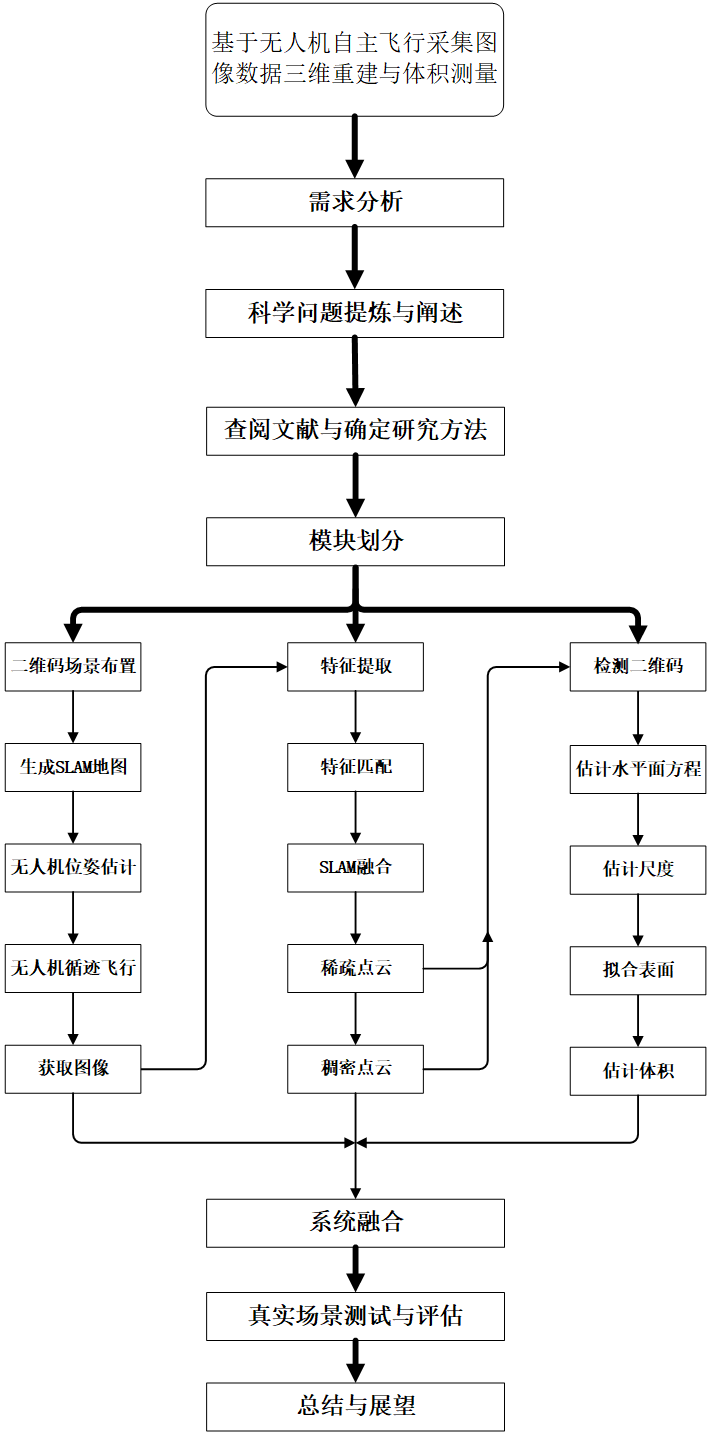
\includegraphics[height=22.5cm]{introduction_pipeline.png}
  \caption{技术路线图}
  \label{fig:introduction_pipeline}
\end{figure}
\section{章节安排}
\label{sec:1.4}


% \chapter{面向堆体测量的无人机自主定位研究}
\label{cha:chap2}
\section{引言}
\label{sec:2.1}
基于SLAM方法的即时建图和定位方法目前已经发展到的相当成熟,尤其是在移动设备定位领域,基于视觉SLAM方法进行定位有着积极的应用。对于实际落地的场景,该系统输出的相机位姿和构建的地图必须具备真实尺度才能够进行导航与定位,此外依靠视觉方法构建的地图,其坐标系往往取决于初始化成功后的第一帧所建立的坐标系,难以与真实世界坐标系有所关联,这些问题的存在都限制着视觉SLAM在实际场景中的存在。

对于单目视觉SLAM算法,设备简易,处理数据较少,满足实时性的要求,但存在无法获取真实世界坐标系下的相机位姿以及无法获取地图实际尺度的问题;对于双目视觉的SLAM算法,可以解决地图尺度的问题,但面临成本较高,相机标定难度大且精度不高,鲁棒性较差等问题;对于融合视觉和IMU传感器的SLAM系统,可以获取真实尺度,以及得到真实世界坐标系下的相机和地图位姿,但该系统对IMU的精度要求较高,存在引入IMU后容易产生累计误差,难以初始化成功等问题。

针对上述问题,本章提出一种面向堆体场景进行测量功能的无人机自主定位方法,该方法将融合二维码视觉标签,在传统SLAM功能的基础上,可以得到相机和地图的真实尺度,并且根据一定的坐标转换,实时获取真实世界坐标系下的相机位姿和地图。在真实的堆体场景中,布置的二维码和普通的自然关键点相比,更加容易捕获,此外,二维码的布置固定,在重定位的流程中,往往会有更好的效果。该系统能够具备以下优良特性:

1. 能够对地图进行保存,复用和更新,通过不断完善的先验地图提高无人机定位的精确度;

2. 引入二维码视觉标签后,通过二维码的先验尺度在仅用单目相机的情况下估计出带有真实尺度的SLAM输出;

3. 结合二维码中坐标系和真实世界的坐标系的转化,可以获取无人机在堆体场景中的实际位姿。
\section{二维码识别与使用方法研究}
\label{sec:2.2}
通过在堆体场景中添加二维码视觉标签,可以使得视觉SLAM算法在实际场景中得以应用,二维码和一般的自然关键点相比较,具备比周围环境更易检出的显著特点,如图~\ref{fig:2VSLAM_MarkerandGradient}所示;且二维码本身是一个四边形的区域,可以凭借该特点估计出相机包含绝对尺度的位姿;并且每一个二维码通过解码都可以获得一个独一无二的ID序号,在SLAM重定位的过程中,可以避免相似区域的的误检情况,在包含二维码的视觉SLAM中,希望尽可能多的检出场景中的二维码视觉标签,随后再通过编码公式对误检值进行剔除。本节将验证二维码得到检测和实现过程,以及如何通过二维码解算相机位姿。
\begin{figure}[H]
  \centering%
  \subcaptionbox{二维码原始图\label{fig:2VSLAM_Marker}}{%    
    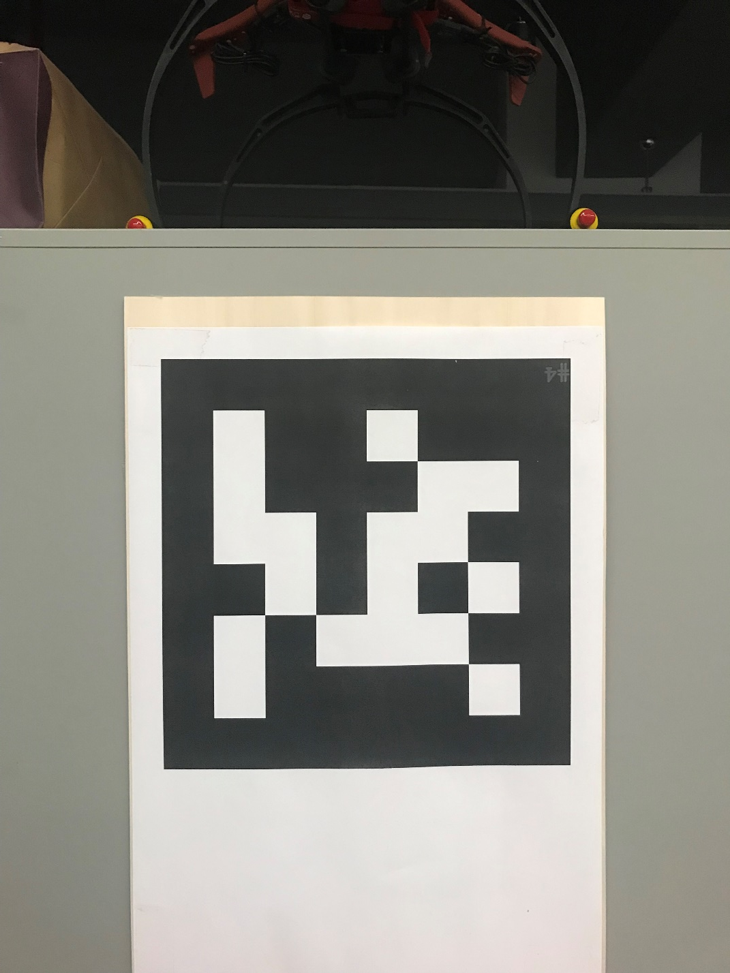
\includegraphics[height=4.5cm]{2VSLAM_Marker.png}}\hspace{1em}%
  \subcaptionbox{二维码梯度图\label{fig:2VSLAM_Marker_Gradient}}{%    
    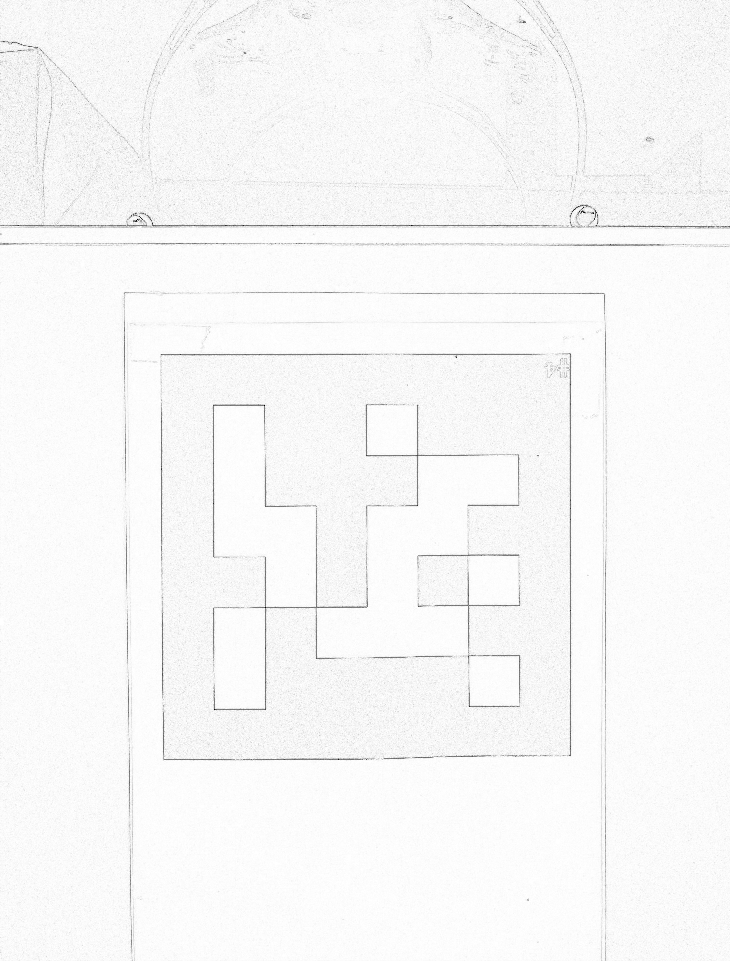
\includegraphics[height=4.5cm]{2VSLAM_Marker_Gradient.png}}
  \caption{二维码原始图和梯度图}
  \label{fig:2VSLAM_MarkerandGradient}
\end{figure}
\subsection{二维码检测与识别过程}
\label{sec:2.2.1}
二维码的检测和识别过程主要包括检测出二维码4个角点在图像中的位置,以及检出二维码对应ID序号,在检测4个角点的位置时,需要检测图像中的线段和构成二维码的四边形。

在线段检测阶段,首先会计算图片中每一个像素梯度强度的大小和方向,随后对计算得到的梯度进行聚类,对所有满足聚类条件的像素点进行合并,得到一组连续点,即检测出线段。

检测完线段后,进一步需要检测构成二维码边缘的四边形,针对上一步中获取到的所有线段,对线段进行分组,若满足,上一线段的末端点和下一线段的起始点之间的距离小于某一阈值,即可首尾按照逆时针进行连接,若所连接的线段数量达到4时,即认定生成的闭环可能为一个二维码的边缘四边形。

在检测二维码ID值之前,会先设定好一个包含所有二维码的字典,字典的大小即包含所有二维码的数量。检测出构成二维码的四边形后,需要对图像进行透视变化规范图像,随后通过设定阈值分离出二维码上的黑色位和白色位,通过位数情况判断出该二维码在字典中对应的特定ID值,识别结果如图~\ref{fig:2VSLAM_Marker_detection}所示。通过这样的方式检测和识别二维码具备非常好的鲁棒性,并且可以对错误值进行筛除。
\begin{figure}[H] % use float package if you want it here
  \centering
  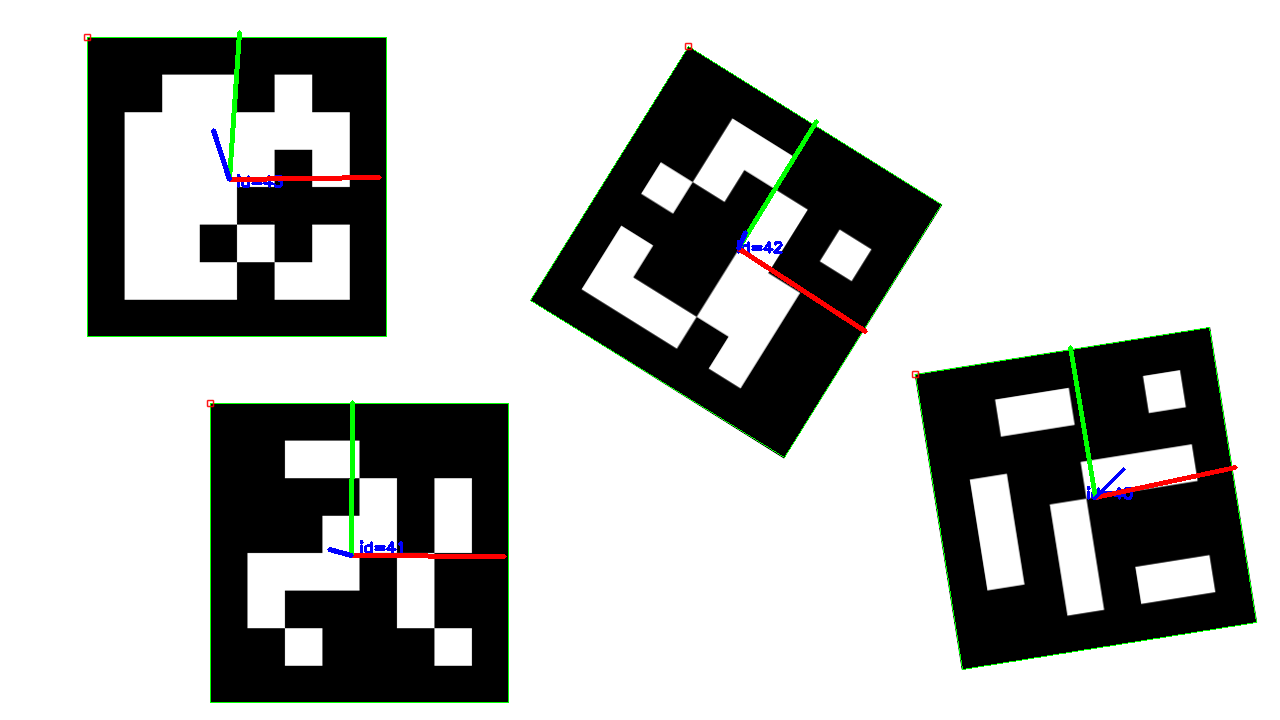
\includegraphics[width=6cm,height=3.8cm]{2VSLAM_Marker_detection.png}
  \caption{二维码识别结果示意图}
  \label{fig:2VSLAM_Marker_detection}
\end{figure} 


\subsection{利用二维码估计相机外参}
\label{sec:2.2.3}
对于单帧图像,在提取完二维码的四边形轮廓,4个角点以及检测出对应的唯一ID值后,接下来可以估计相机位姿,包括平移向量和旋转向量,相机的位姿主要是通过PnP方法来求解。
以二维码坐标系作为世界坐标系,二维码边长为S,则四个角点的坐标分别为A(-S/2,S/2,0),B(S/2,S/2,0),C(S/2,-S/2,0),D(-S/2,-S/2,0),分别在图像中对应的像素点为a($u_a$,$v_a$),b($u_b$,$v_b$),c($u_c$,$v_c$),d($u_d$,$v_d$)。因为相机的内参K提前标定,则三维空间中的点和像素坐标中的点之间的转换关系可以表示为:
\begin{equation}
\begin{split}
  Z{\left[ \begin{array}{ccc}a\\1\end{array} \right ]}=Z{\left[ \begin{array}{ccc}u_a\\v_a\\1\end{array} \right ]}=K{\left[ \begin{array}{ccc}R&t\end{array} \right ]}{\left[ \begin{array}{ccc}A\\1\end{array} \right ]} \\
  ={\left[ \begin{array}{ccc}f_x & 0 & u_0\\0 & f_y &v_0 \\0 & 0 & 1\end{array} \right ]}{\left[ \begin{array}{cccc}r_{11}&r_{12}&r_{13}&t_1\\r_{21}&r_{7722}&r_{23}&t_2\\r_{31}&r_{32}&r_{33}&t_3\end{array} \right ]}{\left[ \begin{array}{ccc} -s/2\\s/2\\0\\1 \end{array} \right ]}
\end{split}
\label{equ:mark2pose}
\end{equation}
通过公式~\ref{equ:mark2pose},可以通过二维码的角点信息求解出相机的旋转矩阵和平移矩阵。
\section{联合二维码的SLAM系统描述}
\subsection{引入二维码对SLAM优化研究}
SLAM是一个在导航的过程中同时进行建图的工作,在使用单目相机时,即使目前表现较好的ORB-SLAM或者LDSO等算法也很难达到预期想要的效果。第一个问题:所构成的地图的尺度未知,这样就造成无法在实际的导航任务中发挥作用;其次,在纯旋转的移动过程中,会导致算法失效;第三个就是单目视觉SLAM往往需要场景中存在比较丰富的材质才能便于跟踪;最后当场景中的视点发生变化,或者场景重复度较高时,对于纯视觉SLAM的重定位,表现效果会很受到很大的限制。

除了用自然点参与视觉SLAM外,还可以使用人为设定的二维码来估计相机位姿,例如SPM-SLAM方法等,该方式可以较好的解决上述问题。因为二维码的放置不需要按照特定的规则,对于堆体场景,可以直接在堆体周围放置二维码标签,这样做就可以的得到一个由二维码构成的地图。但是这样做就需要在场景中布置足够多的二维码视觉标签,那么在大尺度的堆体场景中,这样做就会提高实验的难度,因为在相机移动的过程中,要保证每帧图像中至少有两张二维码出现。

基于上述两种情况,本文提出了一种融合自然特征点和人工放置的二维码的SLAM方法来解决各自的问题和限制。对于实际堆体场景中,结合了自然点和二维码的SLAM方法可以只检测自然点,或者只检测二维码来进行位姿估计。因此对于大多数场景,都可以有更好的鲁棒性,此外,每一个二维码都有一个单独准确得到的ID值,在高度重复的堆体环境中,也能保证匹配的正确性,最后对于大尺度的堆体场景,可以结合自然点进行跟踪,二维码进行重定位来保证SLAM系统的长期稳定。

如图~\ref{fig:2VSLAM_environment}所示,对自然场景进行建图,图~\ref{fig:2VSLAM_environment_cross}为自然区域的原图,在该区域中,部分区域纹理丰富,其余部分则为贫纹理的白墙面,则在白墙面上人为布置二维码标志,图~\ref{fig:2VSLAM_environment_cross_map}为根据该区域重建出的3D地图,可以发现,在丰富纹理的区域,自然点和人为布置的二维码都可以检出,但在贫纹理区域则,则基本只有二维码被检出,因此在贫纹理的区域就可以依靠二维码发挥作用。
\begin{figure}[h]
  \centering
    \subcaptionbox{自然场景示意图\label{fig:2VSLAM_environment_cross}}{
    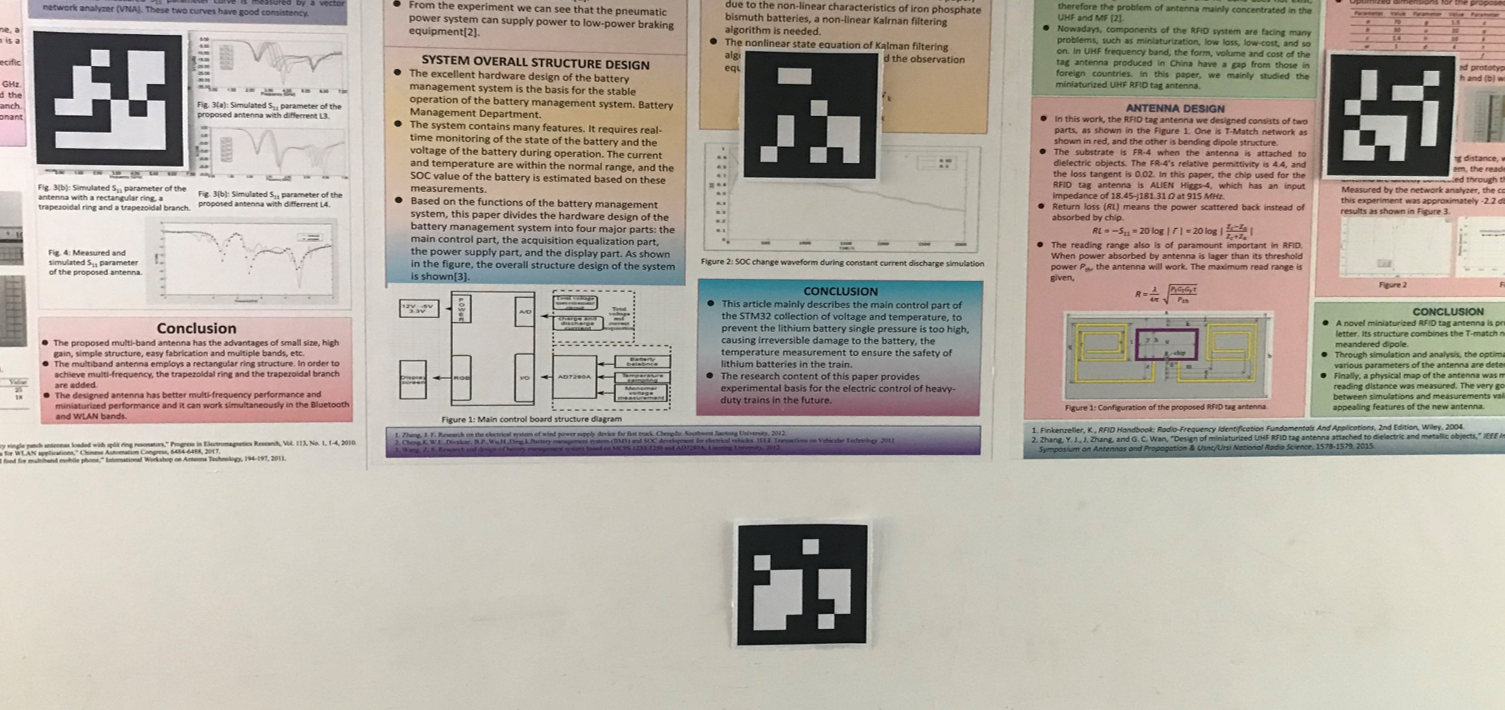
\includegraphics[height=4.5cm,width=9cm]{2VSLAM_environment_cross.png}}
  \vskip0.8cm
    \subcaptionbox{自然场景3D地图\label{fig:2VSLAM_environment_cross_map}}{
    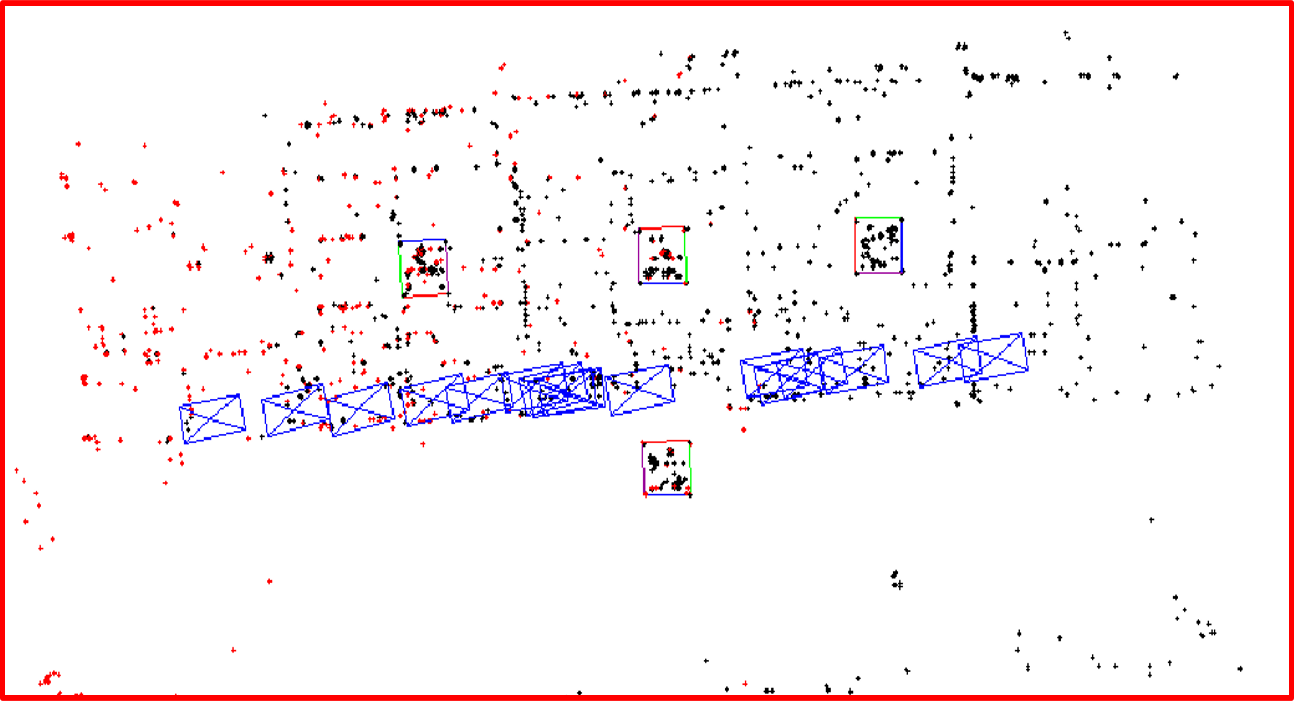
\includegraphics[height=4.5cm,width=9cm]{2VSLAM_environment_cross_map.png}}
  \caption{包含二维码的构建地图示意图}
  \label{fig:2VSLAM_environment}
\end{figure}
\subsection{包含二维码的地图描述}
\label{sec:2.3.2}
在SLAM运行的过程中,可以生成一套地图系统,对于同一场景,该地图可以作为先验复用于后续的建图和定位,通过这样的方式可以添加对系统的约束,提高待估计量的精度。传统SLAM系统组成地图的元素主要包括关键点和关键帧,通过对关键点的描述符进行匹配,可以较好的的估计出相机的位姿。但关键点描述符的计算和匹配过程一般都比较耗时,而且对于堆体场景中,极易出现重复,容易出现出现匹配错误的情况,考虑到这一情况,本文在此基础上,又添加二维码信息作为构成地图的元素,来进一步优化地图以获取更加准确得到相机位姿和地图信息。

本文中地图的构成包括以下3个集合:关键点集合$\mathbf{p}$,关键帧集合$\mathbf{f}$和二维码$\mathbf{f}$集合,每个集合之间的数据元素耦合关联。其中关键点集合
\begin{equation} \mathbf{p}=\{\mathbf{x}, \mathbf{v}, \hat{\mathbf{d}}\}\end{equation}
每个元素代表三维空间中的一个点,该点的描述包括在地图坐标系中的三维坐标$\mathbf{x}$,观测方向$\mathbf{v}$以及该点的描述符信息$\hat{\mathbf{d}}$,考虑到SLAM系统的实时性,选择BRIEF描述符来加快匹配过程。关键帧集合
\begin{equation}\mathbf{f}=\{t, \mathbf{T}, \delta\}\end{equation}
其中每一个关键帧包含一个外参矩阵矩阵$\mathbf{T}$,该外参矩阵是全局参考坐标系到相机参考坐标系的转化,$\delta$是相机的内参矩阵,该参数包括相机焦距,光学中心以及畸变参数,这些参数提前标定。二维码集合
\begin{equation}\mathbf{m}=\left\{s, M, \mathbf{x}^{1}, \mathbf{x}^{2}, \mathbf{x}^{3}, \mathbf{x}^{4}\right\}\end{equation}
其中的每一个二维码包括边长s(需要保证场景中的所有二维码的为正方形且所有二维码的尺度完全一致),二维码由其自身坐标系到全局坐标系的转换矩阵M,$\mathbf{x}^{1}$,$\mathbf{x}^{2}$,$\mathbf{x}^{3}$,$\mathbf{x}^{4}$分别代表二维码四个角点在其自身坐标系下的坐标。通过对包含二维码的自然场景进行离线建图,可以得到如图~\ref{fig:2VSLAM_environment_cross_map}所示的地图,其中正方形代表检出的二维码,蓝色矩形代表检出关键帧,红色点代表检出关键点。

上述地图元素之间还具备一定耦合关系:

1.	对于任意一个关键点,除了自身的属性外,还包括被观测帧序列,即所有可以观测到该特征点的关键帧的集合,以及在这些帧中出现的像素坐标位置

2.	对于任意一个关键帧,还包与其关联的其他关键帧序列,以及在该关键帧中所有观测到的关键点和坐标。

通过这些约束可以使得估计结果有更好的鲁棒性。
\subsection{联合二维码的SLAM过程描述}
\label{sec:2.3.3}
本文所提出的基于二维码的SLAM系统运行框图如图~\ref{fig:2VSLAM_pipeline}所示,与一般SLAM系统相比较,本文主要提出了添加二维码视觉标签的SLAM系统。该系统一直对地图进行维护,有新的信息加入时,则会对更新地图。在对堆体场景运行SLAM时,该地图为空,所以需要对其初始化。
\begin{figure}[H] %  
\centering
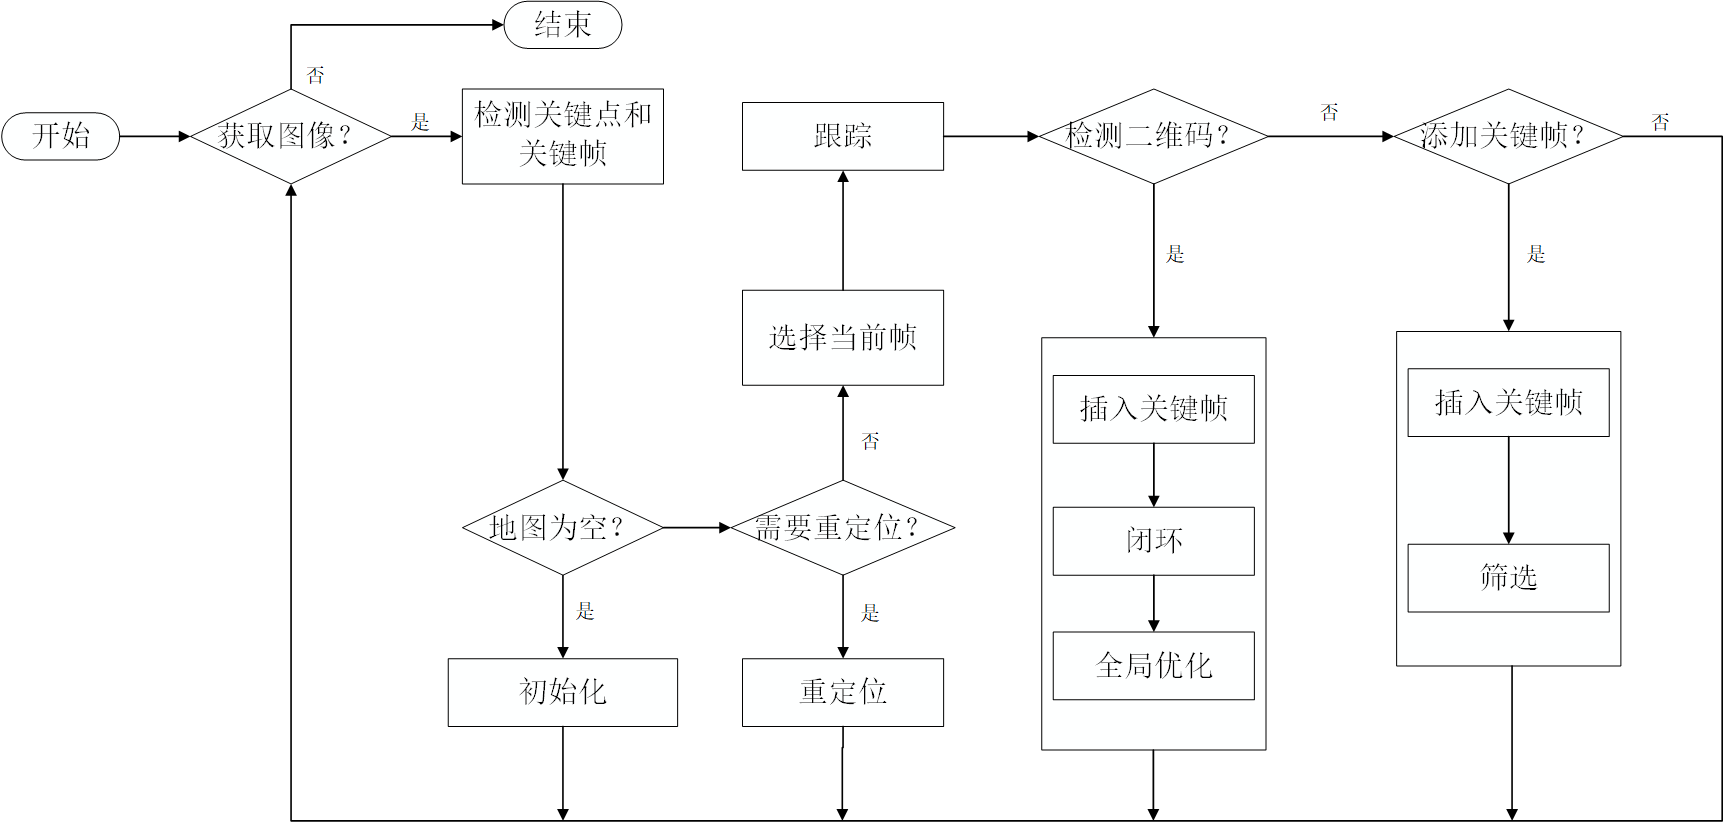
\includegraphics[height=5.7cm,width=11cm]{2VSLAM_pipeline.png}
  \caption{基于二维码的SLAM流程图}
  \label{fig:2VSLAM_pipeline}
\end{figure}
\textbf{地图初始化:}在该SLAM中对地图的初始化可以获取相对尺度信息和参考坐标系的信息,可以依靠图像序列中的关键帧或者二维码来完成,在一般情况下初始化的流程为:首先选择第一和第二帧($f_0$,$f_1$)运行两套初始化方法,如果任意一套方法初始化成功,那么就直接进入跟踪环节;如果两套方案都初始化成功,则优先考虑使用二维码的初始化方式;如果都没有成功,那么则固定第一帧,换取第三帧重复上述过程($f_2$,$f_3$...)。

对于基于二维码的初始化方法,帧之间需要足够的视差,随后得到帧和二维码在地图中的位姿信息,当在某一帧中检测到多个二维码标志时,则可以通过选择在该帧中最小化投影误差最小的二维码来估计初始化信息。使用二维码来进行初始化的一个优点就是,地图中的参数都具备正确的尺度,因此就可以直接用来为无人机的定位提供信息。

\textbf{跟踪模式:}如果在某一帧中估计出相机的位姿,则SLAM系统就会以前一帧作为起始点来估计当前帧的相机位姿,相机的位姿估计是将当前帧中观测到的一组地图三维点和二维码角点进行重投影误差最小化的过程,因此在该过程中主要包括两个步骤:寻找地图的对应关系和通过最小化投影误差获取相机位姿。

在寻找地图点对应关系环节,首先,查找在前一帧中观察到的地图点与参考关键帧之间的匹配,由于该帧很可能再次出现在当前帧中,通过这些匹配可以解算出当前相机的初始估计;然后,通过将地图点投射到参考关键帧的相邻帧中来找到额外的匹配。对于每个地图点,首先需要检查其视角与相机方向之间的夹角是否小于阈值,若大于则丢弃该点,然后,检查相机与地图点之间的欧氏距离是否在关键点的尺度不变性区域内,随后,计算其投影,最后,将地图点的描述符与图像中搜索半径内的关键点进行比较。选择搜索半径中距离最小的两个关键点,且仅当描述符之间的距离比大于0.8,以及最小的描述符距离低于最低阈值$\tau_d$, 则与匹配成功。一旦所有的匹配都被计算出来,重复的匹配就会被移除。最终,关键点结合检测到的二维码标记获得最终的精确位姿。
对于相机的位姿估计,以
\begin{equation}
\Upsilon_{p}^{f}=\{(\mathbf{p}, \mathbf{f}, \mathbf{g})\}
\end{equation}
和
\begin{equation}
\Upsilon_{p}^{\mathrm{f}}=\left\{\left(\mathbf{m}, \mathbf{f}, \mathbf{c}_{\mathbf{m}, \mathbf{f}}\right)\right\}
\end{equation}
表示通过上述步骤得到的$\mathrm{f}$帧中地图点和二维码标记的观测值,对于该帧的位姿$\mathbf{f}_{\mathrm{T}}$可以通过最小化重投影误差来估计:
\begin{equation}
\mathbf{f}_{\mathrm{T}}=\underset{\mathrm{T}}{\operatorname{argmin}}\left(\mathbf{w}_{\mathbf{p}}^{\mathrm{f}} H\left(\Upsilon_{p}^{\mathrm{f}}, \mathrm{T}\right)+\mathbf{w}_{\mathbf{m}}^{\mathrm{f}} H\left(\Upsilon_{m}^{\mathrm{f}}, \mathrm{T}\right)\right)
\label{equ:weight}
\end{equation}
其中
\begin{equation}
H\left(\Upsilon_{m}^{\mathrm{f}}, \mathrm{T}\right)=\sum_{\left(\mathrm{m}, \mathrm{f}, \mathrm{c}_{\mathrm{m}, \mathrm{f}}\right) \in \Upsilon_{m}^{\mathrm{f}}} \sum_{i=1}^{4}\left\|e\left(\mathrm{T} \cdot \mathbf{m}_{\mathrm{M}}, \mathbf{m}_{\mathrm{x}^{i}}, \mathbf{f}_{\delta}, \mathbf{c}_{\mathrm{m}, \mathrm{f}}^{i}\right)\right\|_{2}^{2}
\end{equation}
是当前帧观测到的二维码标记的重投影误差之和,其中
\begin{equation}
H\left(\Upsilon_{p}^{\mathrm{f}}, \mathrm{T}\right)=\sum_{(\mathbf{p}, \mathbf{f}, \mathbf{g}) \in \Upsilon_{p}^{\epsilon}} h_{\alpha}\left(e\left(\mathrm{T}, \mathbf{p}_{\mathbf{x}}, \mathbf{f}_{\delta}, \mathbf{g}_{u}\right) \Omega_{\mathbf{g}} e\left(\mathrm{T}, \mathbf{p}_{\mathbf{x}}, \mathbf{f}_{\delta}, \mathbf{g}_{u}\right)^{\top}\right)
\end{equation}
是当前帧观测到的地图点的重投影误差之和。对于Huber损失函数
\begin{equation}
h_{\alpha}(a)=\left\{\begin{array}{ll}{\frac{1}{2} a^{2}} & {\text { for }|a| \leq \alpha} \\ {\alpha\left(|a|-\frac{1}{2} \alpha\right)} & {\text { otherwise }}\end{array}\right.
\end{equation}
是为了降低优化过程中异常值的相对权重。

对于公式~\ref{equ:weight},二维码视觉标签和地图点的权重分别由
$\mathbf{w}_{\mathbf{m}}^{\mathrm{f}}$
和$\mathbf{w}_{\mathbf{p}}^{\mathrm{f}}$决定,因为同一帧中地图点的数量远远多于二维码的个数,所以必须平衡两者之间的权重,
定义
\begin{equation}
\mathbf{w}_{\mathbf{p}}^{\mathbf{f}}=1-\mathbf{w}_{\mathbf{m}}^{\mathbf{f}}
\end{equation}
和
\begin{equation}
  \mathbf{w}_{\mathbf{m}}^{\mathbf{f}}=\frac{1}{2} \min \left(1, \frac{\mathbf{n}_{\mathbf{f}}}{\tau_{m}}\right)
\end{equation}
其中$\mathbf{n}_{\mathbf{f}}$代表追踪过程中该帧有效的二维码标记的个数,${\tau_{m}}$代表数量阈值,
$\mathbf{w}_{\mathbf{m}}^{\mathbf{f}}$的值将介于$\left[0, \frac{1}{2}\right]$之间,假设在追踪的过程中,没有检测到有效
的二维码,则$\mathbf{n}_{\mathbf{f}}$的值将为0,即该帧的位姿的结果将全部由地图点来估计。

\textbf{插入关键帧:}关键帧只有在向系统添加新信息时才会被添加到地图中,以便实现平稳可靠的跟踪。因此,必须设定一些规则来确定是否需要将当前帧添加至关键帧的集合。本文提出以下关键帧的提取规则:

1. 如果当前帧至少有一个新的二维码标记出现(该标记没有出现在原本的地图中),则将该二维码和该帧添加到地图中。二维码是第一次在该帧中被发现时添加的,因此也不能在帧中明确地估计该二维码的姿态。在这种情况下,标记的位姿被设置为无效,当观察标记的其他关键帧被添加到地图中时,再对其进行估计。

2. 如果该帧包含至少一个二维码标记,且该二维码标记在地图中具有无效位姿,如规则1所描述,则该二维码的位姿可以在该帧中进行估计,则添加该帧并更新该二维码在地图中的位姿。

3. 如果帧包含至少一个二维码标志,并且距当前帧最近的关键帧的距离大于一个阈值$\tau_b$,该帧也会被添加进关键帧。

4. 如果当前帧中匹配的映射点数量低于在参考关键帧中检测到的映射点总数的百分比$\tau_k$,该帧也会被添加进关键帧。

前三条规则的目的是考虑到当前关键帧中的可见二维码视觉标签来检查是否添加关键帧,由于这些规则而没有被认为是关键帧的帧则通过最后一条规则来添加。

本文中的SLAM系统在添加地图点时会遵循一种强鲁棒的策略,当一个新的关键帧被添加到地图时,系统有机会添加新的地图点,以及增加对现有地图点的支持。对于每个关键点,搜索参考关键帧的相邻关键帧之间可能的对应,由于关键帧的姿态是已知的,所以采用了外极限制来减少误检。一旦在地图上添加了一个点,将以一下原则验证该点是否会被加入地图基本思想是,该点必须至少在接下来的三分之二帧中可见,直到再向地图添加两个关键帧。

\textbf{地图优化:}在添加新的关键帧或检测到闭环时,需要更新地图,以便加入新的信息,并剔除不正确的地图点。需要优化的元素包括关键帧位姿$k_T$、地图点位置$p_x$和二维码位姿$m_M$。全局优化是一个缓慢耗时的过程,在SLAM中一般会启用多线程的方式来管理地图。

\textbf{筛选关键帧:}与地图点的保存策略相似,关键帧剔除策略避免了关键帧的无限增长。但是,相似处理关键帧的同时必须同时处理关键点和二维码。其主要流程是,每个二维码和地图点都应至少被三个关键帧所观测到,以便在进行优化过程时实现良好的三角化。对于每一个二维码标记$\mathbf{m}$,从关键帧集合中找到可以观测的关键帧,并筛选出三个和该关键帧距离最近的关键帧,这些关键帧不会被筛除。对于剩余的关键帧,在不显著影响观察到的地图点的情况下会筛选掉,即某个关键帧中的地图点如果存在$\tau_c$的比例以上会被至少三个其他关键帧观测到,那么该帧会被被认为是冗余的,而使用其他三个关键帧代替。

\textbf{回环检测和校准:}在视觉SLAM中,对于相机位姿的解算都是由上一帧来计算的,那么这样就会造成误差的一直传递,产生累积误差,回环检测的提出就是通过建立当前帧和历史帧之间的关系以减少累积误差。词袋模型的提出可以快速简单地完成回环检测,词袋模型使得每一帧都可以用单词来描述,表达为:
\begin{equation}
  F=1 \cdot \omega_{1}+0 \cdot \omega_{2}+0 \cdot \omega_{3}+\ldots+1 \cdot \omega_{n-1}+0 \cdot \omega_{n}
\end{equation}
每一帧$q$都可以由单词$w$和权重$\eta$构成:
\begin{equation}
  A=\left\{\left(w_{1}, \eta_{1}\right),\left(w_{2}, \eta_{2}\right), \ldots,\left(w_{N}, \eta_{N}\right)\right\} \triangleq v_{A}
\end{equation}
可以通过计算$q$,$d$两帧之间字典的相似度判断是否构成回环:
\begin{equation}
  \begin{aligned} s\left(v_{q}, v_{d}\right) &=1-\frac{1}{2}\left|\frac{v_{q}}{\left|v_{q}\right|}-\frac{v_{d}}{\left|v_{d}\right|}\right| \\ &=\frac{1}{2} \sum_{i | q_{i} \neq 0, d_{i} \neq 0}\left(\left|v_{q i}\right|+\left|v_{d i}\right|-\left|v_{q i}-v_{d i}\right|\right) \end{aligned}
\end{equation}

以上是对关键帧的回环处理,对于二维码的回环,必须立即检出由二维码标记引起的闭环,如果在跟踪之前不纠正回环漂移,会导致相机的跟踪问题,因为未纠正的帧位姿可能与二维码所计算出来的位姿差异较大。例如在某一个场景中,系统从一个二维码开始初始化,相机在场景中移动并回到最初的起始位置,在这个过程中,会不断地叠加漂移误差,当相机第二次到达初始位置并再次观察二维码时,估计的相机姿态与实际会较大,当使用二维码标记或关键点检测到循环闭合时,必须纠正漂移。

\textbf{重定位:}如果在跟踪的过程中失败,则必须进行重定位,重定位也是首先考虑使用二维码来完成,如果在某一帧中明确检测到二维码标记,则利用该二维码来重新计算位姿,随后,通过查找地图对应关系和重新估计相机姿态来优化位姿。如果当前帧位姿不能从二维码标记中准确地估计出来,就使用关键帧结合数据库进行查询,查询与当前帧相似的关键帧,并分析最佳关键帧。在回环检测出中,将当前帧的关键帧与所选关键帧进行匹配,并采用RANSACPnP法估计相机的位姿T,如果内置点的数量足够高,则认为重新定位成功,系统重新进入跟踪模式。
\section{面向堆体无人机定位系统设计}
\label{sec:2.4}
\subsection{无人机相机坐标变换数学描述}
\label{sec:2.4.1}
% 在SLAM系统中,常用的坐标系存在2个概念,分别是相机坐标系和世界坐标系。其中世界坐标系是我们最需要考虑的一个坐标系,世界坐标系代
% 表的是真实世界下,物体所参考的坐标系,一般都是固定不动的,可以给运动的物体提供控制方法,对于世界中的任意一点,可以描述
% 为P($X_w$,$Y_w$,$Z_w$)。相机坐标系代表的是移动的物体自身的坐标系,由于相机是刚性物体,一般以相机的坐标为准,对于相机中的任何一点,可
% 以描述为P($X_c$,$Y_c$,$Z_c$)。

% 因为SLAM系统中会涉及到多个坐标系,不同的坐标系之间需要进行转化,空间中点的坐标系变换是一个欧式变换,一般由旋转加平移构成。首先
% 只考虑坐标的纯旋转问题,即只有旋转,没有平移产生,两个坐标系的基底分别为($\vec {e_1}$,$\vec {e_2}$,$\vec {e_3}$)和
% ($\vec {e'_ 1}$,$\vec {e'_2}$,$\vec {e'_3}$)对应的坐标分别为($\vec {a_1}$,$\vec {a_2}$,$\vec {a_3}$)和($\vec {a'_1}$,$\vec {a'_2}$,$\vec {a'_3}$)。则有:
% \begin{equation}
% \begin{array}{l}\begin{bmatrix}\overrightarrow{e_1}&,\overrightarrow{e_2}&,\overrightarrow{e_3}\end{bmatrix}
% \begin{bmatrix}a_1\\a_2\\a_3\end{bmatrix}=\begin{bmatrix}\overrightarrow{e_1'}&,\overrightarrow{e_2'}&,\overrightarrow{e_3'}\end{bmatrix}
% \begin{bmatrix}a_1'\\a_2'\\a_3'\end{bmatrix}\\a\;=
% \begin{bmatrix}a_1\\a_2\\a_3\end{bmatrix}\;=
% \begin{bmatrix}e_1^Te_1'&e_1^Te_2'&e_1^Te_3'\\e_2^Te_1'&e_2^Te_2'&e_2^Te_3'\\e_3^Te_1'&e_3^Te_2'&e_3^Te_3'\end{bmatrix}
% \begin{bmatrix}a_1'\\a_2'\\a_3'\end{bmatrix}=Ra'\\\end{array}
% \end{equation}
% 其中旋转矩阵R由两组基之间的内积组成,表示坐标系旋转前后同一个向量的坐标变换关系。旋转矩阵是一个行列式为1的正交矩阵,满足以下特点:
% \begin{equation}RR^T=E(I),det(R)=I\end{equation}
% 则有:
% \begin{equation}a'=R^{-1}a=R^Ta\end{equation}
% 在欧式变换中,除了旋转还有平移:
% \begin{equation}a'=Ra+t\end{equation}
% 可以用旋转矩阵R和平移向量t就能描述空间中的坐标变换关系
% \begin{equation}
% \begin{bmatrix}a'\\1\end{bmatrix}=
% \begin{bmatrix}R&t\\0^T&1\end{bmatrix}
% \begin{bmatrix}a\\1\end{bmatrix}=T
% \begin{bmatrix}a\\1\end{bmatrix}
% \end{equation}
% 在三维向量的末尾添加1,称为齐次坐标。矩阵T同时包含了旋转和平移,称为变换矩阵。

人机上携带的相机可以看成三维空间中的刚体(保证了同一个向量在各个坐标系下的长度和夹角都不会发生变化),对于相机的平移和旋转,平移可以利用向量来表示,旋转则利用旋转矩阵,旋转向量,欧拉角,四元数等方式来描述,本文也将主要说明旋转过程的数学描述。

\textbf{旋转矩阵:}对于任意向量{~p~},在两个坐标系的描述为:
\begin{equation}
  \left[\mathbf{e}_{1}, \mathbf{e}_{2}, \mathbf{e}_{3}\right]\left[\begin{array}{l}{a_{1}} \\ {a_{2}} \\ {a_{3}}\end{array}\right]=\left[\mathbf{e}_{1}^{\prime}, \mathbf{e}_{2}^{\prime}, \mathbf{e}_{3}^{\prime}\right]\left[\begin{array}{c}{a_{1}^{\prime}} \\ {a_{2}^{\prime}} \\ {a_{3}^{\prime}}\end{array}\right]
\end{equation}
等式两边同时左乘$\left[\begin{array}{ccc}{\mathbf{e}_{1}^{T},} & {\mathbf{e}_{2}^{T},} & {\mathbf{e}_{3}^{T}}\end{array}\right]^{T}$可得
\begin{equation}
\left[\begin{array}{l}{a_{1}} \\ {a_{2}} \\ {a_{3}}\end{array}\right]=\left[\begin{array}{lll}{e_{1}^{T} e_{1}^{\prime}} & {e_{1}^{T} e_{2}^{\prime}} & {e_{1}^{T} e_{3}^{\prime}} \\ {e_{2}^{T} e_{1}^{\prime}} & {e_{2}^{T} e_{2}^{\prime}} & {e_{2}^{T} e_{3}^{\prime}} \\ {e_{3}^{T} e_{1}^{\prime}} & {e_{3}^{T} e_{2}^{\prime}} & {e_{3}^{T} e_{3}^{\prime}}\end{array}\right]\left[\begin{array}{c}{a_{1}^{\prime}} \\ {a_{2}^{\prime}} \\ {a_{3} ;}\end{array}\right]=\mathbf{R a}^{\prime}
\end{equation}
对于旋转矩阵R,可描述旋转过程,并且R可以定义为特殊正交群:
\begin{equation}
  S O(n)=\left\{\mathbf{R} \in R^{n \times n} | \mathbf{R} \mathbf{R}^{T}=\mathbf{I}, \operatorname{det}(\mathbf{R})=1\right\}
\end{equation}

\textbf{旋转向量:}旋转矩阵在描述旋转时存在参数冗余和自身约束的问题,因此提出一个更加紧凑的数学描述$\theta_{n}$,旋转向量方向为旋转轴{~n~},
大小为旋转角$\theta$。旋转向量和旋转矩阵的转换可以用罗德里格斯公式表示:
\begin{equation}
  \mathbf{R}=\cos \theta \mathbf{I}+(1-\cos \theta) \mathbf{n} \mathbf{n}^{T}+\sin \theta \mathbf{n}^{\wedge}
\end{equation}
反之则有
\begin{equation}
  \operatorname{tr}(\mathbf{R})=\cos \theta \operatorname{tr}(\mathbf{I})+(1-\cos \theta) \operatorname{tr}\left(\mathbf{n} \mathbf{n}^{T}\right)+\sin \theta \operatorname{tr}\left(\mathbf{n}^{\wedge}\right)=1+2 \cos \theta
\end{equation}
\textbf{欧拉角:}将旋转运动分解成分别绕三个坐标轴的旋转($[r, p, y]^{T}$)来表示的,三个旋转的总和即为总的旋转,表述最为直观。

\textbf{四元数:}由于欧拉角和旋转向量存在奇异性,且不存在不带奇异性的三维向量描述方式,因此提出四元数这种紧凑且没有奇异性的数学描述。四元数可以描述为:
\begin{equation}
  \mathbf{q}=q_{0}+q_{1} i+q_{2} j+q_{3} k=\{s, \mathbf{v}\}
\end{equation}
可以用单位四元数来描述空间中的任意旋转,假设旋转的描述为$\theta_{n}$,则:
\begin{equation}
  \mathbf{q}=\left[\cos \frac{\theta}{2}, n_{x} \sin \frac{\theta}{2}, n_{y} \sin \frac{\theta}{2}, n_{z} \sin \frac{\theta}{2}\right]^{T}
\end{equation}
旋转描述为R时,则:
\begin{equation}
\mathbf{R}=\left[\begin{array}{ccc}{1-2 q_{2}^{2}-2 q_{3}^{2}} & {2 q_{1} q_{2}-2 q_{0} q_{3}} & {2 q_{1} q_{3}+2 q_{0} q_{2}} \\ {2 q_{1} q_{2}+2 q_{0} q_{3}} & {1-2 q_{1}^{2}-2 q_{3}^{2}} & {2 q_{2} q_{3}-2 q_{0} q_{1}} \\ {2 q_{1} q_{3}-2 q_{0} q_{2}} & {2 q_{2} q_{3}+2 q_{0} q_{1}} & {1-2 q_{1}^{2}-2 q_{2}^{2}}\end{array}\right]
\end{equation}
反之则有:
\begin{equation}
  q_{0}=\frac{\sqrt{\operatorname{tr}(\mathbf{R})+1}}{2}, q_{1}=\frac{m_{23}-m_{32}}{4 q_{0}}, q_{2}=\frac{m_{31}-m_{13}}{4 q_{0}}, q 3=\frac{m_{12}-m_{21}}{4 q_{0}}
\end{equation}
通过以上方式都可以描述刚性运动中的旋转过程R,结合物体的平移t,则变化后的坐标为:
\begin{equation}
  \mathbf{a}^{\prime}=\mathbf{R} \mathbf{a}+\mathbf{t}
\end{equation}
在实际的使用中,由于以上等式非线性,可以引入齐次坐标T,可以将上式改成:
\begin{equation}
\left[\begin{array}{l}{\mathbf{a}^{\prime}} \\ {1}\end{array}\right]=\left[\begin{array}{ll}{\mathbf{R}} & {\mathbf{t}} \\ {\mathbf{0}^{T}} & {1}\end{array}\right]\left[\begin{array}{l}{\mathbf{a}^{\prime}} \\ {1}\end{array}\right]=\mathbf{T}\left[\begin{array}{l}{\mathbf{a}} \\ {1}\end{array}\right]
\end{equation}
对于变换矩阵T,可以定义为特殊欧氏群:
\begin{equation}
S E(3)=\left\{T=\left[\begin{array}{cc}{\mathbf{R}} & {\mathbf{t}} \\ {\mathbf{0}^{T}} & {1}\end{array}\right] \in R^{4 \times 4} | \mathbf{R} \in S O(3), t \in R^{3}\right\}
\end{equation}

对于针孔相机模型,如图~\ref{fig:2VSLAM_pinehole}所示,(其中f为相机焦距)存在4个坐标系分别为:世界坐标系,相机坐标系,图像坐标系和像素坐标系,对于真实世界中的空间点$P_w$($X_w$,$Y_w$,$Z_w$),其对应的相机坐标系坐标为$P_c$($C_w$,$C_w$,$C_w$),对应的图像坐标系为$P^{'}$($X^{'}$,$Y^{'}$),对应的像素坐标系为p(u,v)。
\begin{figure}[H]
  \centering
  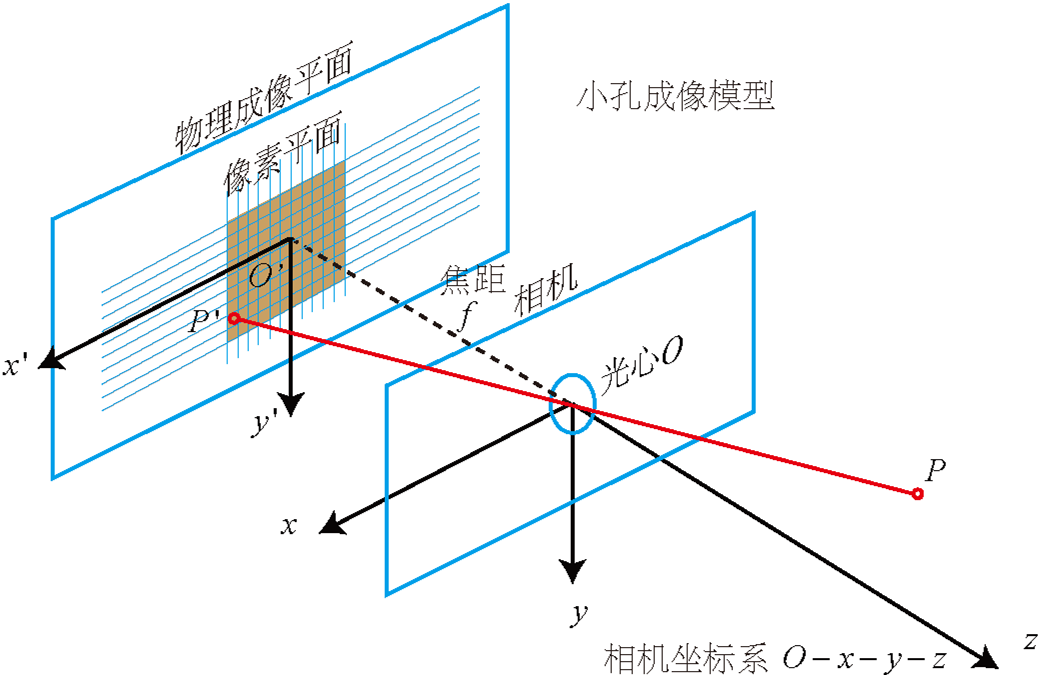
\includegraphics[height=4.5cm]{2VSLAM_pinehole.png}
  \caption{针孔相机模型}
  \label{fig:2VSLAM_pinehole}
\end{figure}
对于世界坐标系到相机坐标系之间的转化:
\begin{equation}
  \left[\begin{array}{l}{X c} \\ {Y_{C}} \\ {Z_{C}}\end{array}\right]=R\left[\begin{array}{l}{X w} \\ {Y w} \\ {Z w}\end{array}\right]+t
  \label{equ:world2cam}
\end{equation}
对于相机坐标系到图像坐标系之间的转化,可以利用如图~\ref{fig:2VSLAM_similartri}所示的相似三角形来求解:
\begin{equation}
  \begin{split}
    \frac{Z c}{f}=\frac{X c}{X^{'}}=\frac{Y c}{Y^{'}}\\
    \left\{\begin{array}{l}{X^{\prime}=f \frac{X c}{Z c}} \\ {Y^{\prime}=f \frac{Y c}{Z c}}\end{array}\right.
\end{split}
\label{equ:cam2photo}
\end{equation}
对于图像坐标系到像素坐标系的转化,如图~\ref{fig:2VSLAM_pixeltrans}所示:
\begin{equation}
  \begin{split}
    \left\{\begin{array}{l}{u=\frac{X^{\prime}}{d_{x}}+u_{o}} \\ {v=\frac{Y^{\prime}}{d_{y}}+v_{o}}\end{array}\right.\\
    \left[\begin{array}{l}{u} \\ {v} \\ {1}\end{array}\right]=\left[\begin{array}{ccc}{\frac{1}{d_{x}}} & {0} & {u_{o}} \\ {0} & {\frac{1}{d_{x}}} & {v_{o}} \\ {0} & {0} & {1}\end{array}\right]\left[\begin{array}{c}{X^{\prime}} \\ {Y^{\prime}} \\ {1}\end{array}\right]
  \end{split}
  \label{equ:photo2pixel}
\end{equation}
\begin{figure}[H]
  \centering%
  \subcaptionbox{相机坐标系到图像坐标系转换\label{fig:2VSLAM_similartri}}{%    
    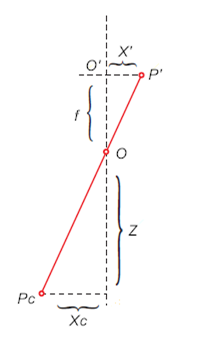
\includegraphics[height=4cm]{2VSLAM_similartri.png}}\hspace{6em}%
  \subcaptionbox{图像坐标系到像素坐标系转换\label{fig:2VSLAM_pixeltrans}}{%    
    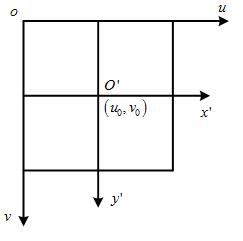
\includegraphics[height=4cm]{2VSLAM_pixeltrans.png}}
  \caption{坐标系转化示意图}
  \label{fig:trans}
\end{figure}
其中$d_x$,$d_y$分别表示沿着x,y轴的实际物理尺寸,($u_o$,$v_o$)表示光心对应到像素坐标系得到坐标.由公式~\ref{equ:cam2photo}和
~\ref{equ:photo2pixel}可以转化得到相机坐标系到像素坐标系的关系:
\begin{equation}
Z c\left[\begin{array}{l}{u} \\ {v} \\ {1}\end{array}\right]=\left[\begin{array}{ccc}{\frac{f}{d_{x}}} & {0} & {u_{0}} \\ {0} & {\frac{f}{d_{y}}} & {v_{0}} \\ {0} & {0} & {1}\end{array}\right]\left[\begin{array}{c}{X_{c}} \\ {Y_{c}} \\ {Z_{c}}\end{array}\right]=\left[\begin{array}{ccc}{f_{x}} & {0} & {u_{0}} \\ {0} & {f_{y}} & {v_{0}} \\ {0} & {0} & {1}\end{array}\right]\left[\begin{array}{c}{X_{c}} \\ {Y_{c}} \\ {Z_{c}}\end{array}\right]=K\left[\begin{array}{c}{X_{c}} \\ {Y_{c}} \\ {Z_{c}}\end{array}\right]
  \label{equ:cam2pixel}
\end{equation}
由公式~\ref{equ:world2cam}和~\ref{equ:cam2pixel}得到世界坐标系到像素坐标系的转化关系为:
\begin{equation}
Z c\left[\begin{array}{l}{u} \\ {v} \\ {1}\end{array}\right]=K(R P w+t)=K\left(R\left[\begin{array}{l}{X w} \\ {Y w} \\ {Z w}\end{array}\right]+t\right)
\end{equation}
其中K表示相机内参矩阵,R,t表示相机外参。 

\subsection{获取真实世界坐标系方法}
\label{sec:2.4.2}
在SLAM系统中所描述的定位信息都是基于地图坐标系或者相机坐标系,但是在实际的应用中,就需要将所有的定位信息全部转换至真实世界坐标系下,才能为无人机后续的移动提供控制方法。传统的SLAM方法,只能够得获取相机在地图坐标系下的位姿,本文结合二维码自带坐标系的特性,可以经过一定的转换获取相机在真实世界坐标系下的位姿,为后续控制提供真实世界下的位姿信息。

首先,声明所有可以得到的坐标信息,二维码在SLAM地图坐标系下的位姿$T_{marker}^{c}$,相机在SLAM地图坐标系下得到位姿$T_{camera}^{c}$,二维码在真实世界坐标系的位姿$T_{marker}^{w}$。

经过坐标变化,可以的得到相机在二维码下的位姿
\begin{equation}
T_{camera}^{m} =\begin{bmatrix}T_{marker}^{c}\end{bmatrix}^{-1}T_{camera}^{c}
\end{equation}
真实世界坐标系在二维码坐标系下的位姿
\begin{equation}
T_{world}^{m} =\begin{bmatrix}T_{marker}^{w}\end{bmatrix}^{-1}
\end{equation}
那么相机在真实世界坐标系下的位姿
\begin{equation}
\begin{array}{l}T_{camera}^w=
\begin{bmatrix}T_{world}^m\end{bmatrix}^{-1}T_{camera}^m\\=\;T_{marker}^w
\begin{bmatrix}T_{marker}^c\end{bmatrix}^{-1}T_{camera}^c\end{array}
\end{equation}
其中,二维码在真实世界坐标系的位姿可以按照实际场景进行设置,为了计算方便,直接设定第一个二维码的中心点为世界坐标系三维坐标的中心点,且x轴朝右,y轴朝上,z轴垂直于二维码平面向外,如图~\ref{fig:2VSLAM_global}所示,那么第一个二维码的在世界坐标系下的坐标为(0,0,0),其余二维码则可以按照真实尺度获取。
\begin{figure}[H] % use float package if you want it here
  \centering
  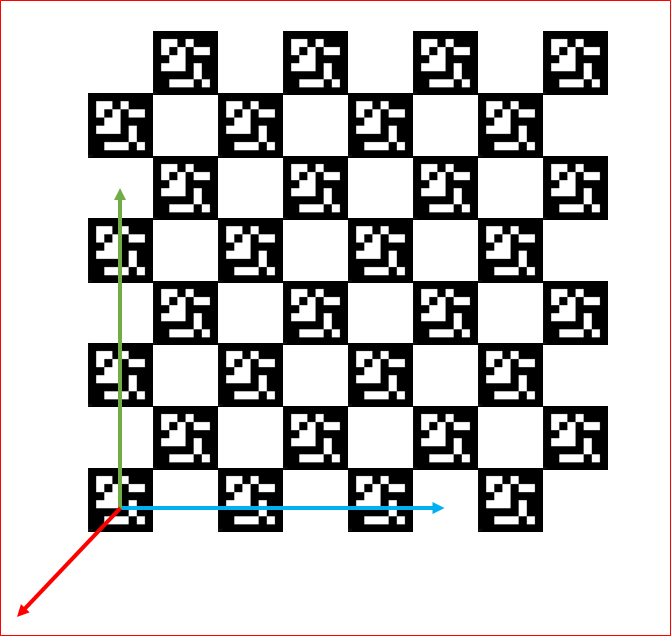
\includegraphics[height=6cm]{2VSLAM_global.png}
  \caption{二维码布置示意图}
  \label{fig:2VSLAM_global}
\end{figure}

在SLAM实际运行前,应该保证二维码的实际布置坐标和设定的二维码在实际世界坐标系下的坐标一致,避免SLAM过程中位姿的抖动问题,先验地图可以以配置文件的形式记录,这样可以针对不同的场景和不同的二维码布置情况,直接修改配置文件即可。在SLAM运行过程中,应该尽可能保证每一帧都可以看到至少一个二维码,,对于观测不到二维码的图像帧,SLAM算法将利用特征点匹配进行定位,当观测的图像帧中有多个二维码时,那么就需要考虑到多个二维码的协同影响,本文提出以下几种处理形式:

1. 提前选择某一个参考二维码,无论相机观测到哪一个二维码,都根据观测到的二维码和参考二维码之间的位姿关系,求解相机在世界坐标系下的位姿。

2. 对于观测到的多个二维码标记,根据上一帧计算出来的位姿,可以计算出当前帧距离最近的一个二维码,以该二维码作为参考,计算出此时相机在世界坐标系下的位姿。

3. 对于观测到的多个二维码标记,分别结合各个二维码计算出此时相机在世界坐标系下的位姿,对于所有位姿,求取平均值即可。

以上三种方法都可以解算出相机在真实世界坐标系下的位姿,其中方法1的计算过程最为简略,并且全程只利用一个参考二维码可以避免在频繁更换参考二维码的过程中造成的位姿抖动问题,但是会存在线性放大相机位姿误差的情况,该方法难以对误差进行优化。方法2会应用到历史位姿信息,可以有效降低相机位姿估计的误差,但会频繁更换参考二维码,这样也会造成相机位姿估计过程的抖动问题。方法3.和方法2类似,在处理误差时会结合多个参考二维码的信息,使得估计位姿的系统鲁棒性提升。针对不同的场景,需要结合具体的方法,对于二维码远距离线性摆放的场景,应该避免使用方法1,优先考虑方法2和方法3;对于实时性要求较高的场景,则优先考虑方法1。

% \begin{algorithm}[!h]
  % 	\caption{PARTITION$(A,p,r)$}%算法标题
  % 	\begin{algorithmic}[1]%一行一个标行号
  % 		\STATE $i=p$
  % 		\FOR{$j=p$ to $r$}
  % 		\IF{$A[j]<=0$}
  % 		\STATE $swap(A[i],A[j])$
  % 		\STATE $i=i+1$
  % 		\ENDIF
  % 		\ENDFOR
  % 	\end{algorithmic}
  % \end{algorithm}
\subsection{无人机自主定位设计}
\label{sec:2.4.3}
在根据以上章节,可以确定出在真实世界下相机的位姿结果,在具体的工程实践中,除了结合二维码的SLAM算法的研究,还需要考虑到先验地图的设定,数据的传输,相机的设定等问题,具体流程如图\ref{fig:2VSLAM_getPose_pipeline}所示。
\begin{figure}[h] % use float package if you want it here
  \centering
  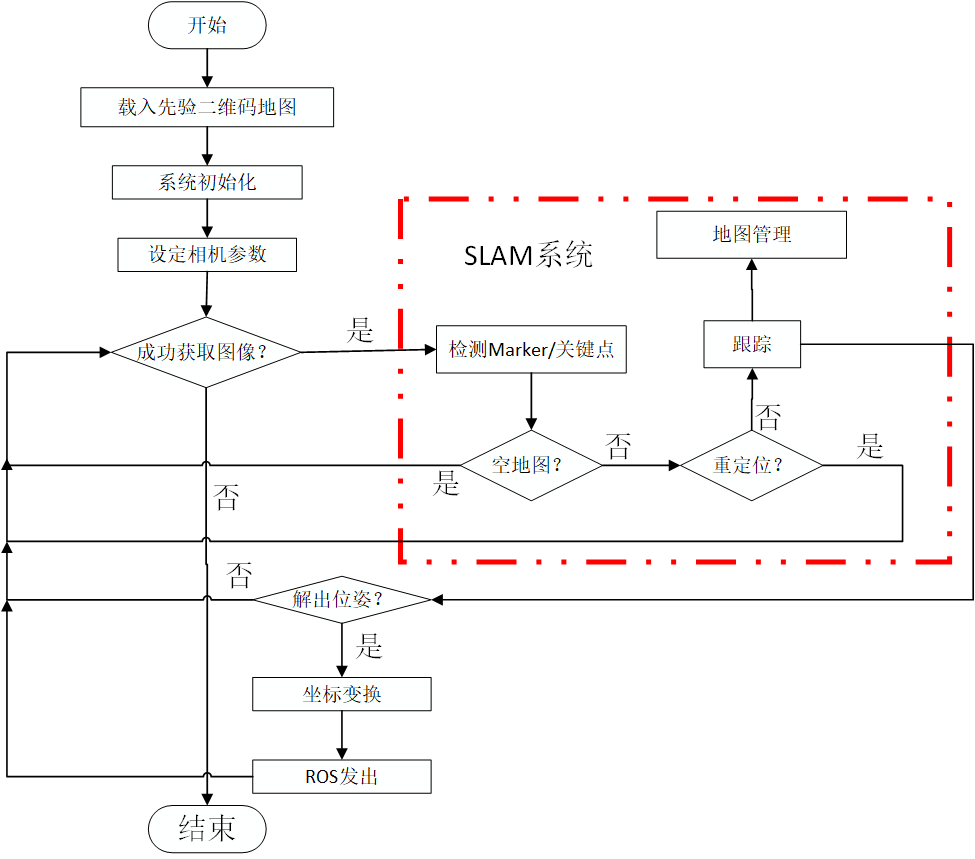
\includegraphics[height=10cm]{2VSLAM_getPose_pipeline.png}
  \caption{获取真实位姿完整流程图}
  \label{fig:2VSLAM_getPose_pipeline}
\end{figure}

\textbf{地图管理:}在无人估计位姿时,如果有先验地图的加入,则可以添加约束进一步优化位姿结果。在载入地图的过程中,如果该场景是第一次测量,没有先验的地图信息,则创建一个空的globalmap来存储地图信息,并将MapFlag字段设定为NotFirstMap;反之,则直接载入历史先验地图。在整个定位流程结束后,将更新后的地图保存在globalmap中,代码如~\ref{code: Map_Process}所示。
\begin{lstlisting}[
  language=C++,
  numbers=left,                
  numberstyle=\footnotesize,
  frame=single,     
  basicstyle=\small\tt,    
  escapeinside = '',
  caption={地图管理~C++~实现},
  label={code: Map_Process}]
'//载入地图'
if (Map_Flag == NotFirst_Map) 
	{
    globalmap->readFromFile(map_path);
  }
else
	{
    globalmap->readFromFile(map_path);
	  Map_Flag == NotFirst_Map;
	}
'//保存地图'
if (Map_Flag == Save_Map) 
    {globalmap->saveToFile(map_path);}
\end{lstlisting}
\textbf{载入先验二维码地图:}首先准备先验地图配置文件,包括二维码的真实尺度,所有二维码的ID值,以及每一个二维码特定的id值和在真实世界坐标系下的位姿(R,t)。如代码~\ref{code:loadMarkermap}所示,需要依次遍历每个二维码的信息,最终将所有数据都存储在markermap中。
\begin{lstlisting}[
  language=C++,
  numbers=left,                
  numberstyle=\footnotesize,
  frame=single,     
  basicstyle=\small\tt,    
  escapeinside = '',
  caption={载入先验二维码地图~C++~实现},
  label={code:loadMarkermap}]

'先验地图配置文件:'
  %YAML:1.0
  markersize: 0.73
  markers_id: [0,1]
  id_0: !!opencv-matrix
  rows: 4
  cols: 4
  dt: d
  data: [1.0, 0.0, 0.0, 0.0, 
        0.0, 1.0, 0.0, 0.0,  
        0.0, 0.0, 1.0, 0.0, 
        0.0, 0.0, 0.0, 1.0]
  id_1: !!opencv-matrix
  rows: 4
  cols: 4
  dt: d
  data: [1.0, 0.0, 0.0, 4.0, 
          0.0, 1.0, 0.0, 0.0,  
          0.0, 0.0, 1.0, 0.0, 
          0.0, 0.0, 0.0, 1.0]

'先验地图载入代码:'
  void loadMarkermap(string path){
    cv::FileStorage fs(path, cv::FileStorage::READ);
    fs["markersize"] >> markersize;
    fs["markers_id"] >> markers_id;
    for (std::size_t  i =0;i<markers_id.size();i++){
        cv::Mat cvmarker ;
        Eigen::Matrix<double,4,4> marker;
        fs["id_"+to_string(markers_id[i])] >> cvmarker;
        cv2eigen(cvmarker,marker);
        markermap[markers_id[i]] = marker;
    }
  }
\end{lstlisting}
\textbf{设定SLAM参数:}对于结合二维码的SLAM系统,需要对系统中的参数进行设定,主要包括SLAM的运行模式(SLAM模式,重定位模式),特征点的提取方式(orb、brief、SIFT等),二维码的检测类别(ARUCO\_MIP\_25h7、ARUCO\_MIP\_36h12等),关键帧筛选阈值,线程的数量,是否复用地图等等,这些SLAM相关的参数都需要在运行前设定,具体内容如代码~\ref{code:setSlam}所示。
\begin{lstlisting}[
  language=C++,
  numbers=left,                
  numberstyle=\footnotesize,
  frame=single,     
  basicstyle=\small\tt,    
  escapeinside = '',
  caption={slam启动和参数设置~C++~实现},
  label={code:setSlam}]
  void setSlam(int argc){
      UcoSlamParams.runSequential=false;
      UcoSlamParams.detectMarkers=true;
      UcoSlamParams.aruco_markerSize=markersize;
      UcoSlamParams.aruco_Dictionary="ARUCO_MIP_36h12";
      UcoSlamParams.nthreads_feature_detector =1;
  }
\end{lstlisting}
\textbf{设定相机参数:}相机的选择对基于纯视觉的无人机定位任务也很重要,作为SLAM系统的输入,必须选择一台成像质量高,稳定性强的相机。在实际工程中选择PointGrey (CM3-U3-31S4M-CS)工业相机来接受视觉信息,外形如图~\ref{fig:2VSLAM_pointgrey}所示,具体参数如表~\ref{tab:pointgrey}所示。
\begin{figure}[H] 
  \centering
  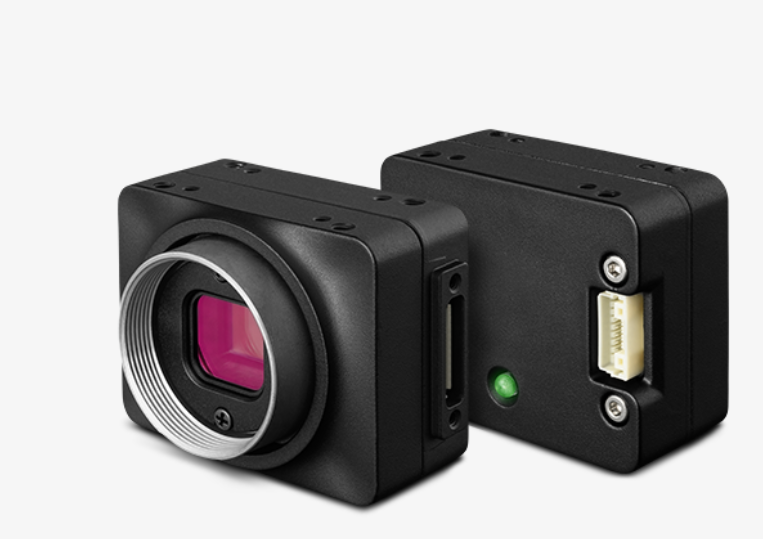
\includegraphics[height=4.5cm]{2VSLAM_pointgrey.png}
  \caption{PointGrey工业相机示意图}
  \label{fig:2VSLAM_pointgrey}
\end{figure}
\begin{table}[h]
  \centering
  \caption{pointgrey相机参数表}
  \label{tab:pointgrey}
  \begin{tabular}{C{1.6cm}C{2.4cm}C{2.6cm}C{6.4cm}}
  \toprule
  \textbf{参数} & \textbf{数值} & \textbf{参数} & \textbf{数值} \\
  \midrule
  Frame Rate       & 30 FPS       & Megapixels      & 1.3 MP            \\
  Lens Mount       & CS-mount     & Readout Method  & Global shutter           \\
  Sensor Format    & 1/3"         & Chroma          & Color        \\
  Sensor Type      & CCD 	        & Part Number     & CM3-U3-13S2C-CS           \\
  Pixel Size       & 3.75 µm   	  & Sensor Name     & Sony ICX445      \\
  Resolution       & 1288 × 964	  & Required Accessories & Lens, Cable, Host Adapter (USB 3.1 Gen 1), Tripod Mount Adapter (ACC-01-0003)        \\

  \bottomrule
  \end{tabular}
\end{table}
相机在使用过程中需要设定的参数一般包括相机内参,以及曝光,快门时间和增益等,对于相机内参需要提前进行标定,后面三个参数需要根据实际场景调试后确定出最佳数值,代码如~\ref{code:setCamera}所示

\begin{lstlisting}[
  language=C++,
  numbers=left,                
  numberstyle=\footnotesize,
  frame=single,     
  basicstyle=\small\tt,    
  escapeinside = '',
  caption={相机参数设定~C++~实现},
  label={code:setCamera}]
  int SHUTTER=7 ; int BRIGHTNESS=0.5; float GAIN=20.0;
  void setCamera(){
    for (int frameNumber = 0; ;frameNumber++) {
        char key = static_cast<char>(cv::waitKey(1));
        if ( key =='w' || key == 'W') {break;}
        if ( key =='u' || key == 'U'){SHUTTER =SHUTTER+1;}
        if ( key =='j' || key == 'J'){SHUTTER =SHUTTER-1;}
        if ( key =='i' || key == 'I'){BRIGHTNESS =BRIGHTNESS+1;}
        if ( key =='k' || key == 'K'){BRIGHTNESS =BRIGHTNESS-1;}
        if ( key =='o' || key == 'O'){GAIN =GAIN+1;}
        if ( key =='l' || key == 'L'){GAIN =GAIN-1;}
        mypointgrey->pointgreyInit(SHUTTER,BRIGHTNESS,GAIN);
        mypointgrey->getData();
    }
  }
\end{lstlisting}
\textbf{设定数据传输系统:}在工程实践中,一般都采用ROS(机器人操作系统)来对数据进行传输,其用于编写机器人软件程序的一种具备高灵活轻度的软件架构,可以使得数据在多个进程中进行传输,本文主要涉及SLAM进程和无人机飞控进程,这两个进程分别对同一个节点进行数据得到发布和订阅以完车数据传输,代码如~\ref{code:setROS}所示。
\begin{lstlisting}[
  language=C++,
  numbers=left,                
  numberstyle=\footnotesize,
  frame=single,     
  basicstyle=\small\tt,    
  escapeinside = '',
  caption={ROS初始化设定和数据传输~C++~实现},
  label={code:setROS}]
void publishPose(ros::Publisher odom_pub){
    Eigen::Quaterniond q = Eigen::Quaterniond(t.block<3,3>(0,0));      
    nav_msgs::Odometry odometry;
    ros::Time current_time= ros::Time::now();
    odometry.header.stamp = current_time;
    odometry.header.frame_id = "world";
    odometry.pose.pose.position.x = t(0,3);
    odometry.pose.pose.position.y = t(1,3);
    odometry.pose.pose.position.z = t(2,3);
    odometry.pose.pose.orientation.x = q.x();
    odometry.pose.pose.orientation.y = q.y();
    odometry.pose.pose.orientation.z = q.z();
    odometry.pose.pose.orientation.w = q.w();
    odom_pub.publish(odometry);  
    ros::spinOnce();        
}

for (int frameNumber = 0; keyPressed!=27;frameNumber++) {
  ...\dots
  publishPose(odom_pub);   
}

ros::init(argc, argv, "talker");  
ros::NodeHandle n;  
ros::Publisher odom_pub = 
              n.advertise<nav_msgs::Odometry>("odom", 1000);      
ros::Rate loop_rate(10);  
\end{lstlisting}

根据以上流程,可以针对堆体,在不适用GPS的条件下进行无人机的自主定位和控制,无人机所拍摄的堆体场景如图~\ref{fig:2VSLAM_big}所示。二维码视觉标签位于图像左侧,连续放置,为无人机的自主定位提供世界坐标系得到真实位姿。
\begin{figure}[t]
  \centering
      \subcaptionbox{Frame1}{\label{fig:2VSLAM_big1}
      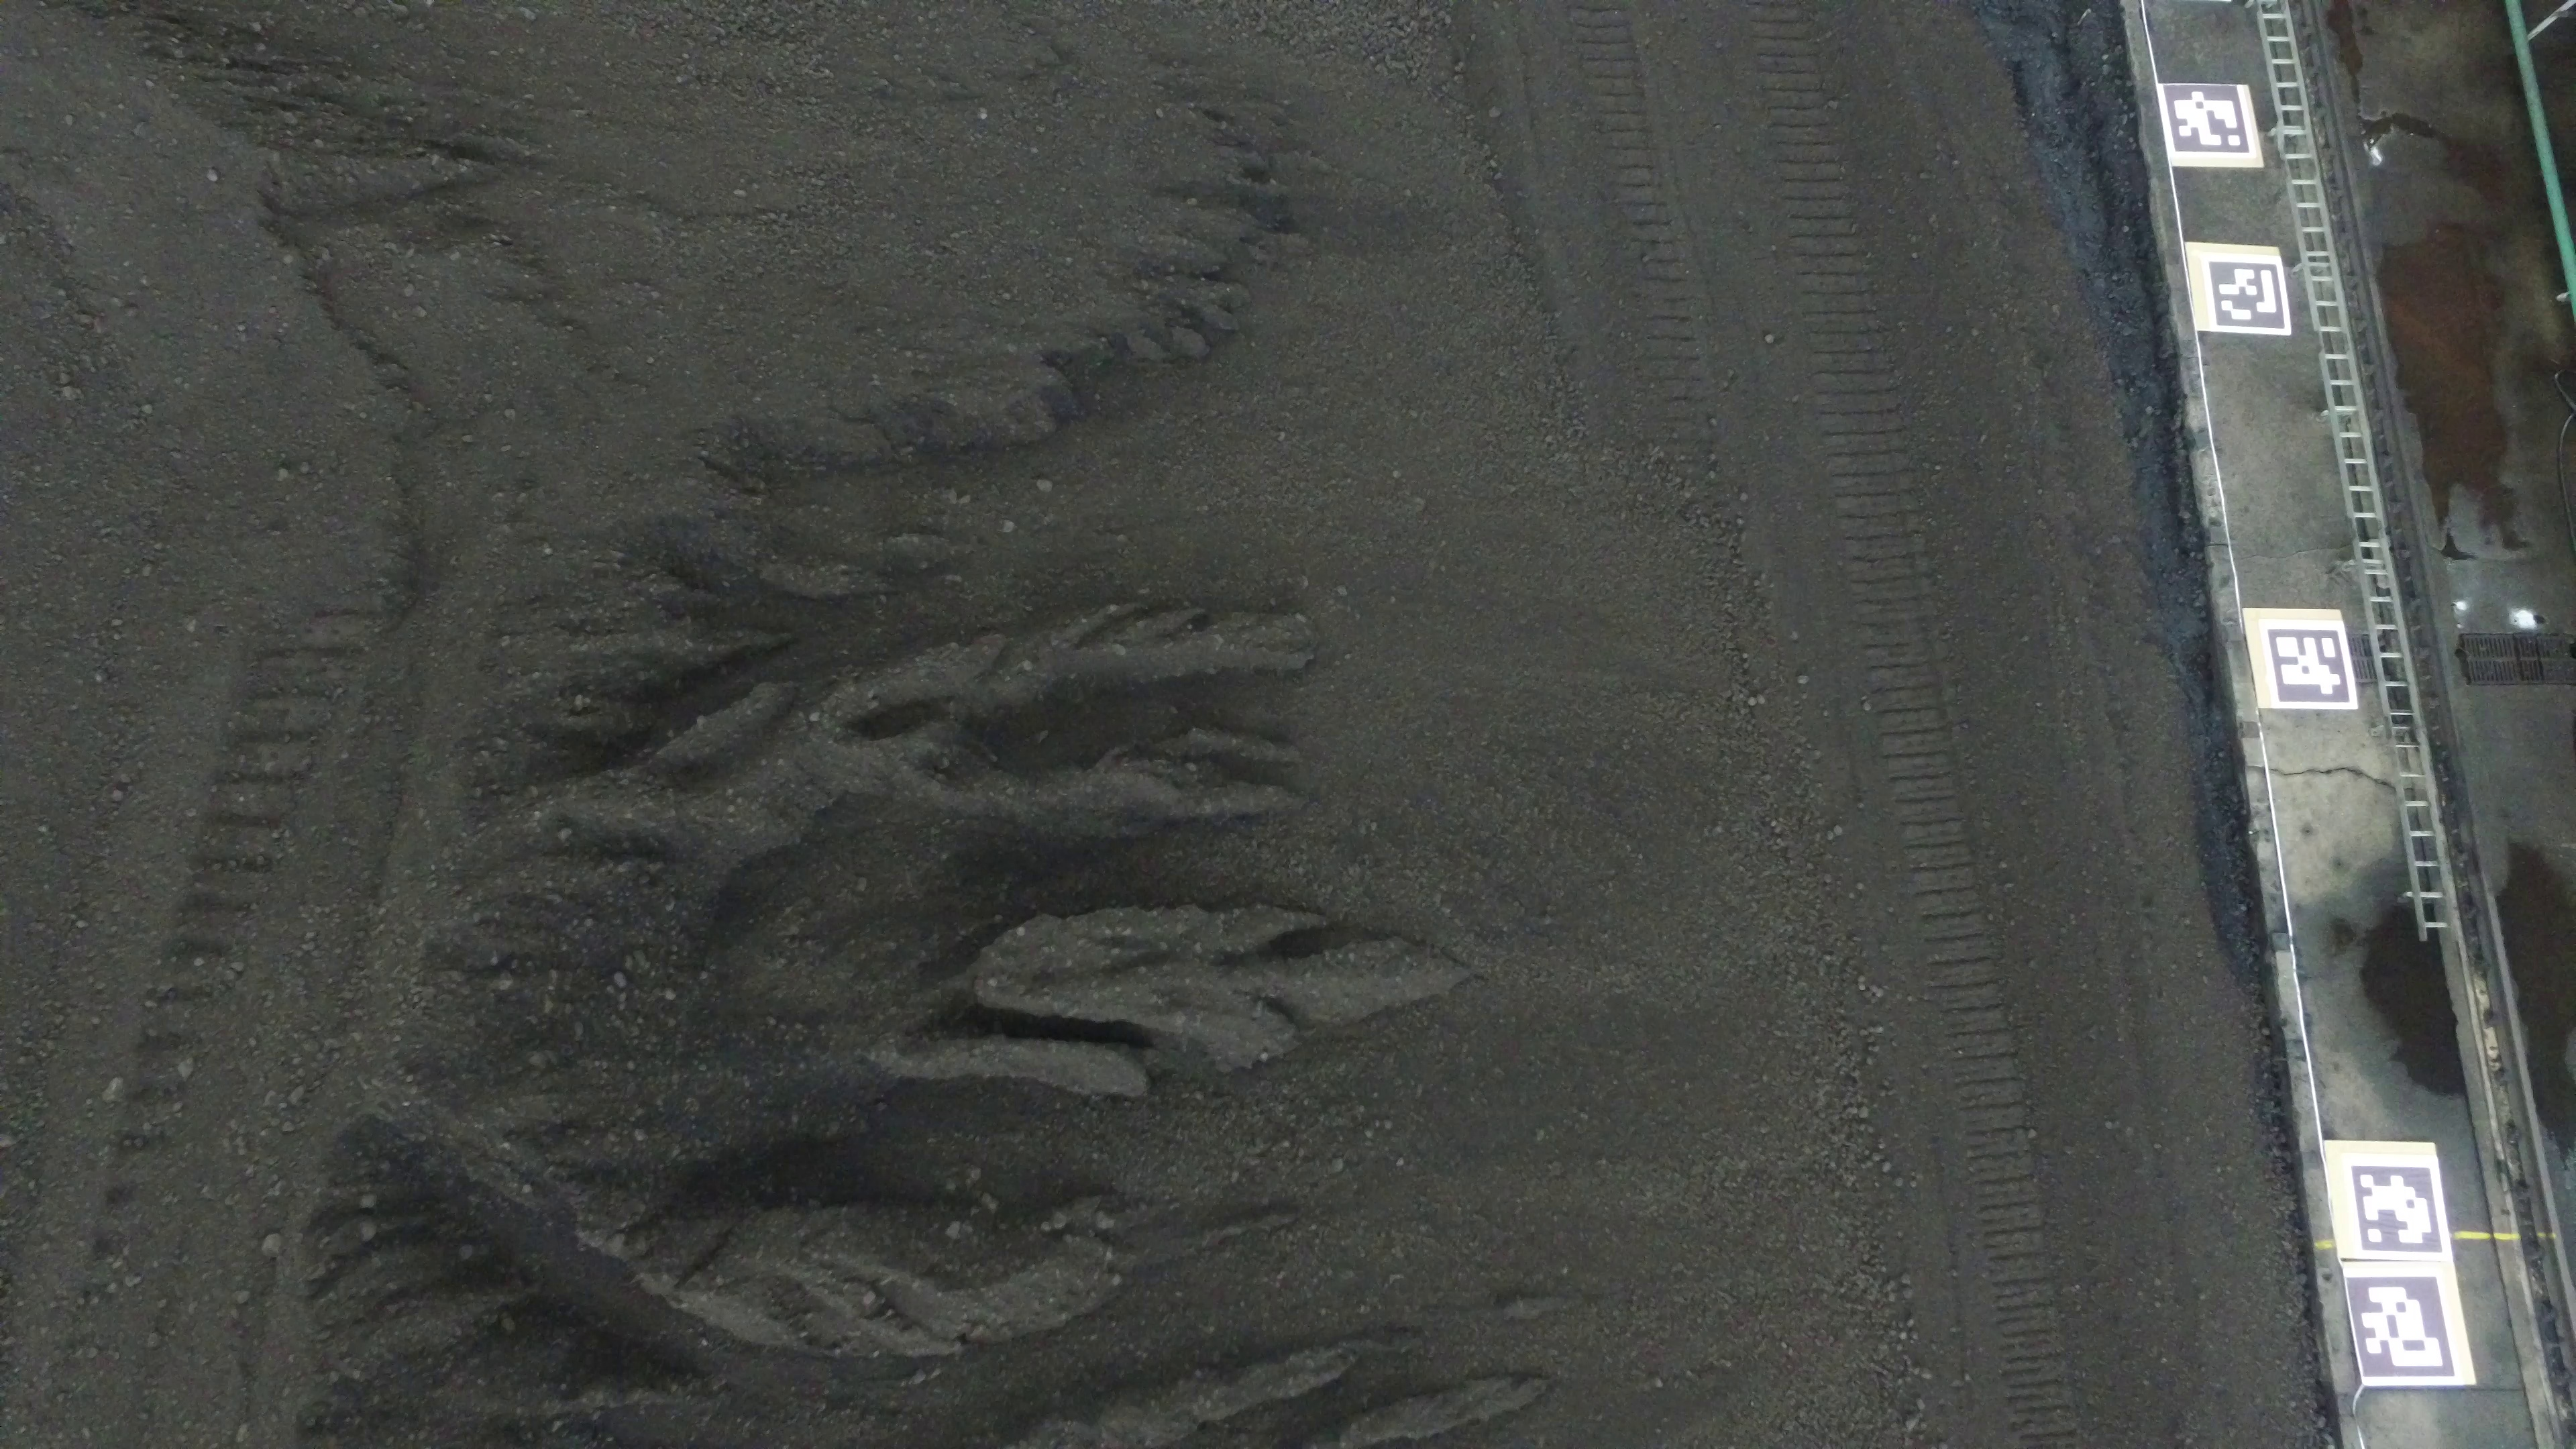
\includegraphics[width=4cm]{2VSLAM_big1.jpg}\hskip1cm}
      \subcaptionbox{Frame2}{\label{fig:2VSLAM_big2}
      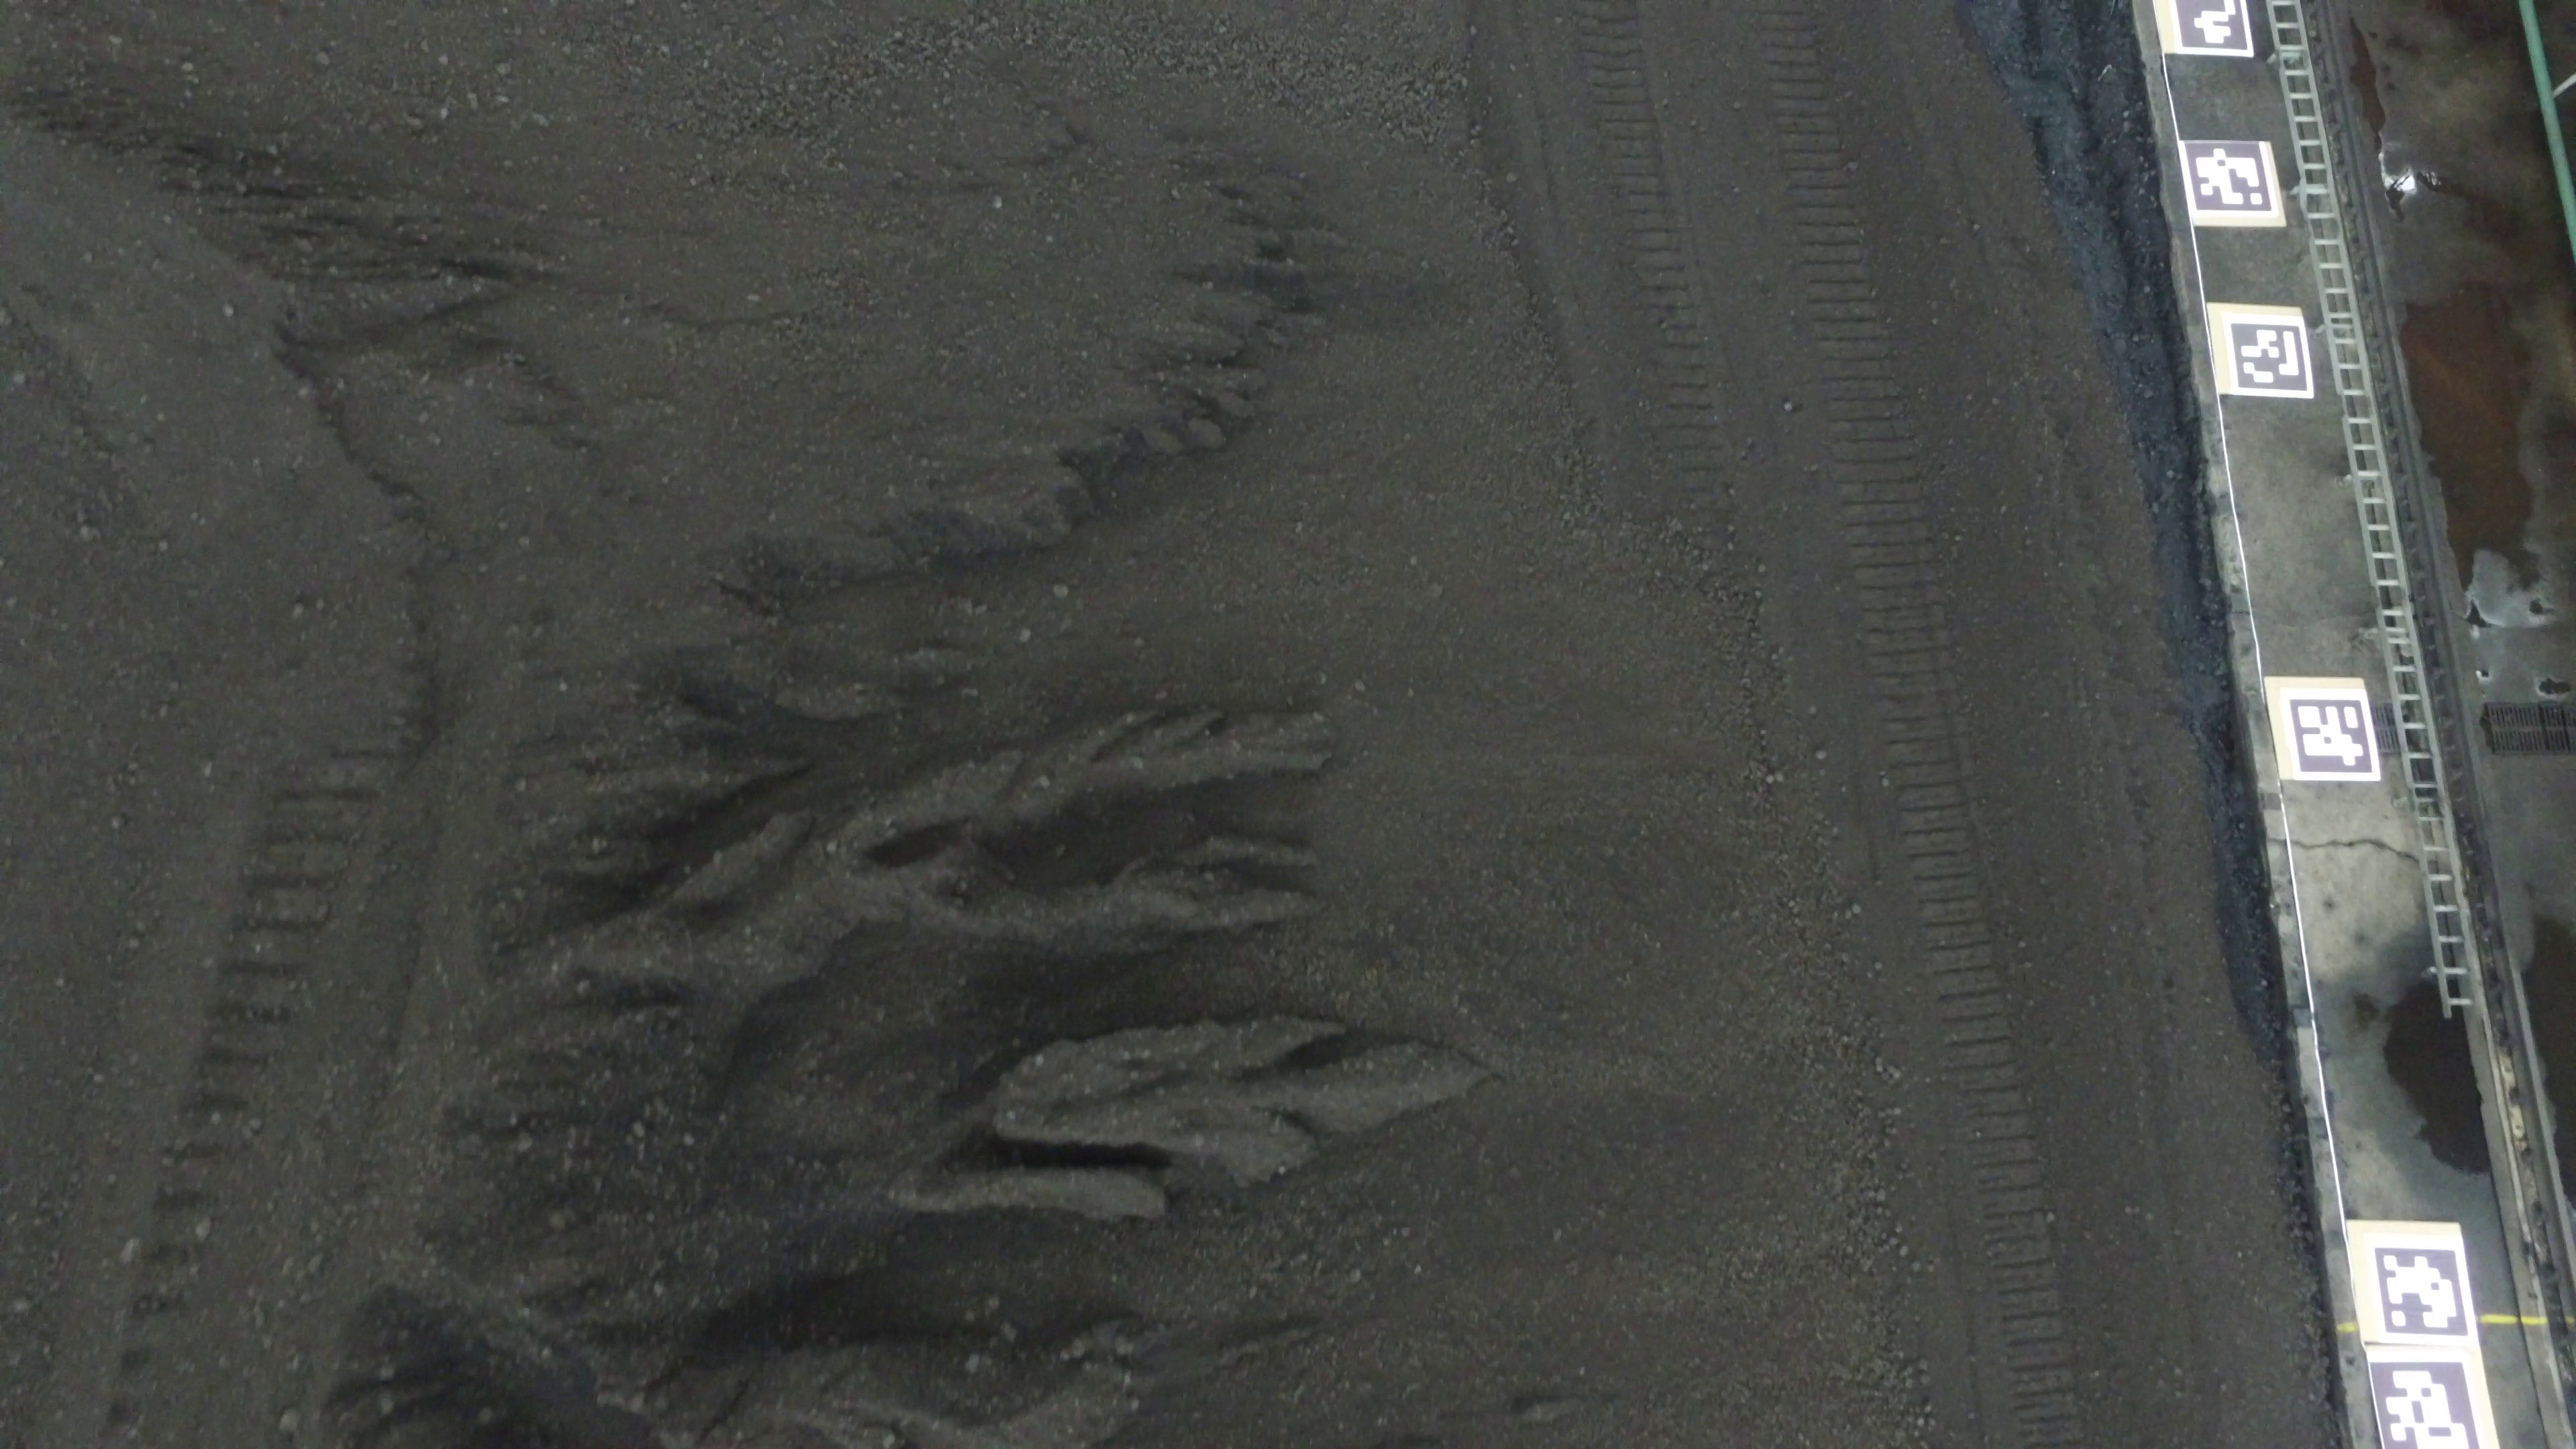
\includegraphics[width=4cm]{2VSLAM_big2.jpg}\hskip1cm}
      \subcaptionbox{Frame3}{\label{fig:2VSLAM_big2}
      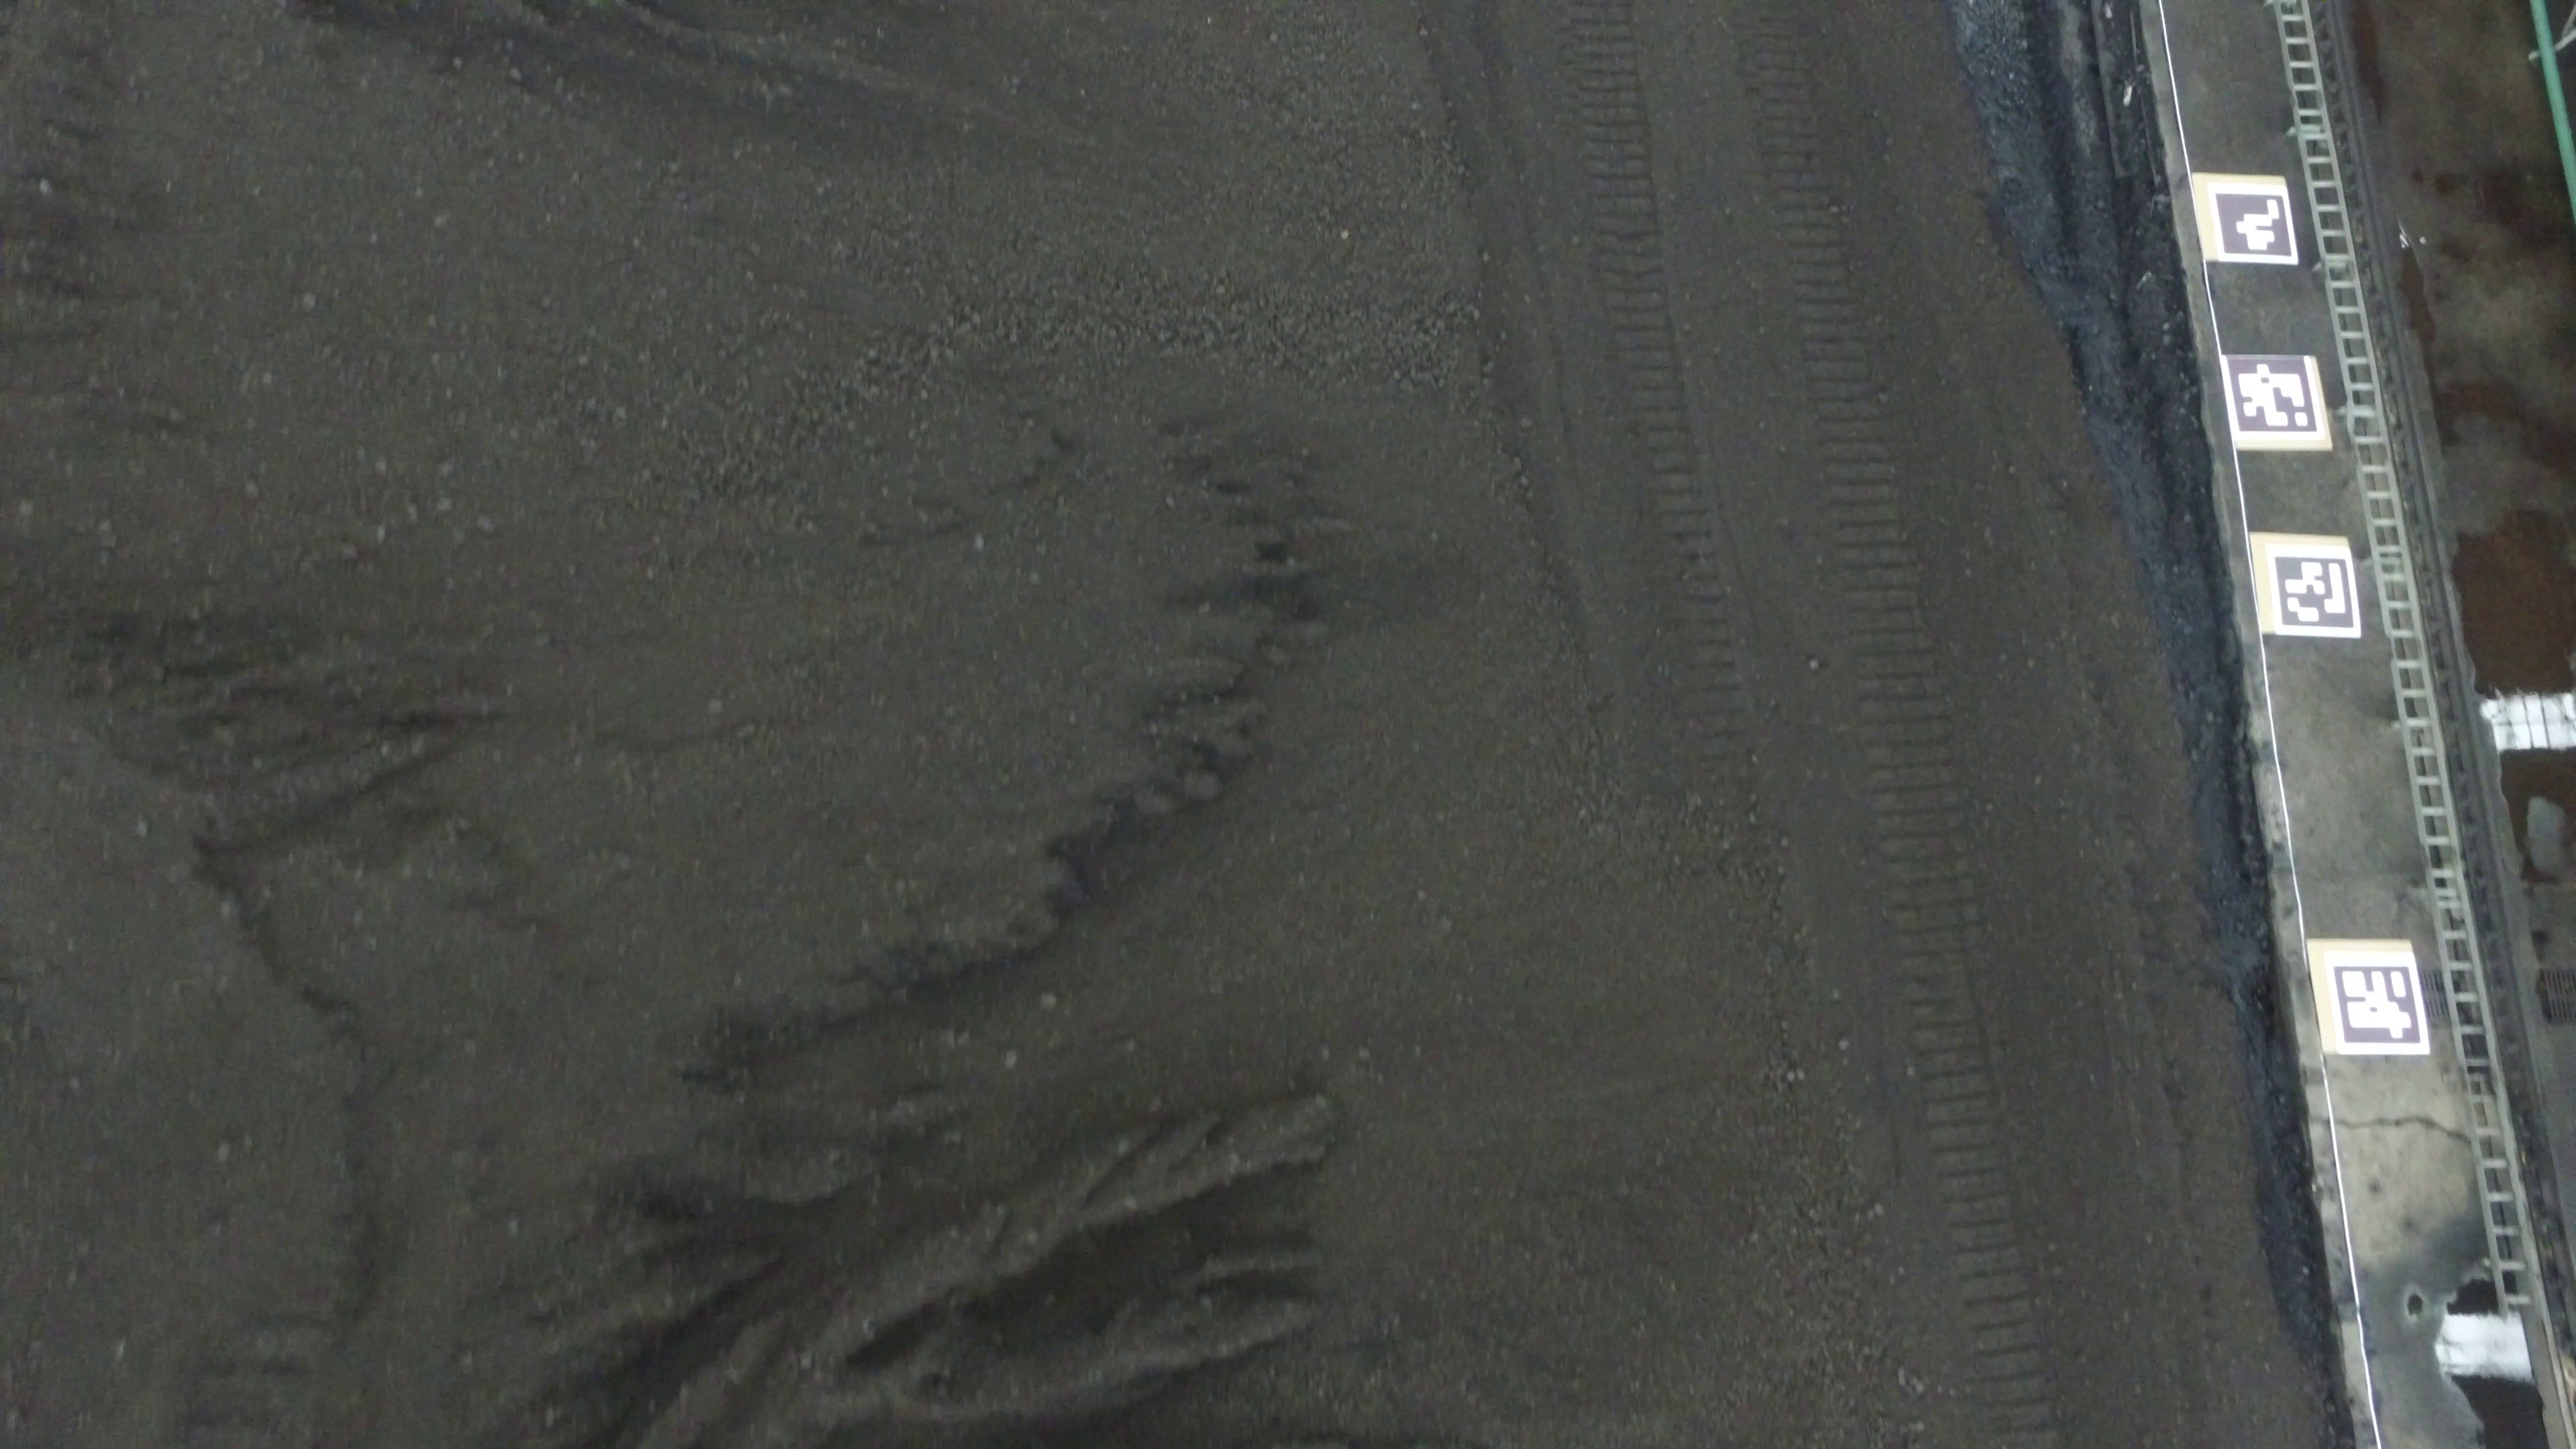
\includegraphics[width=4cm]{2VSLAM_big3.jpg}}
    \vskip0.2cm
      \subcaptionbox{Frame4}{\label{fig:2VSLAM_big4}
      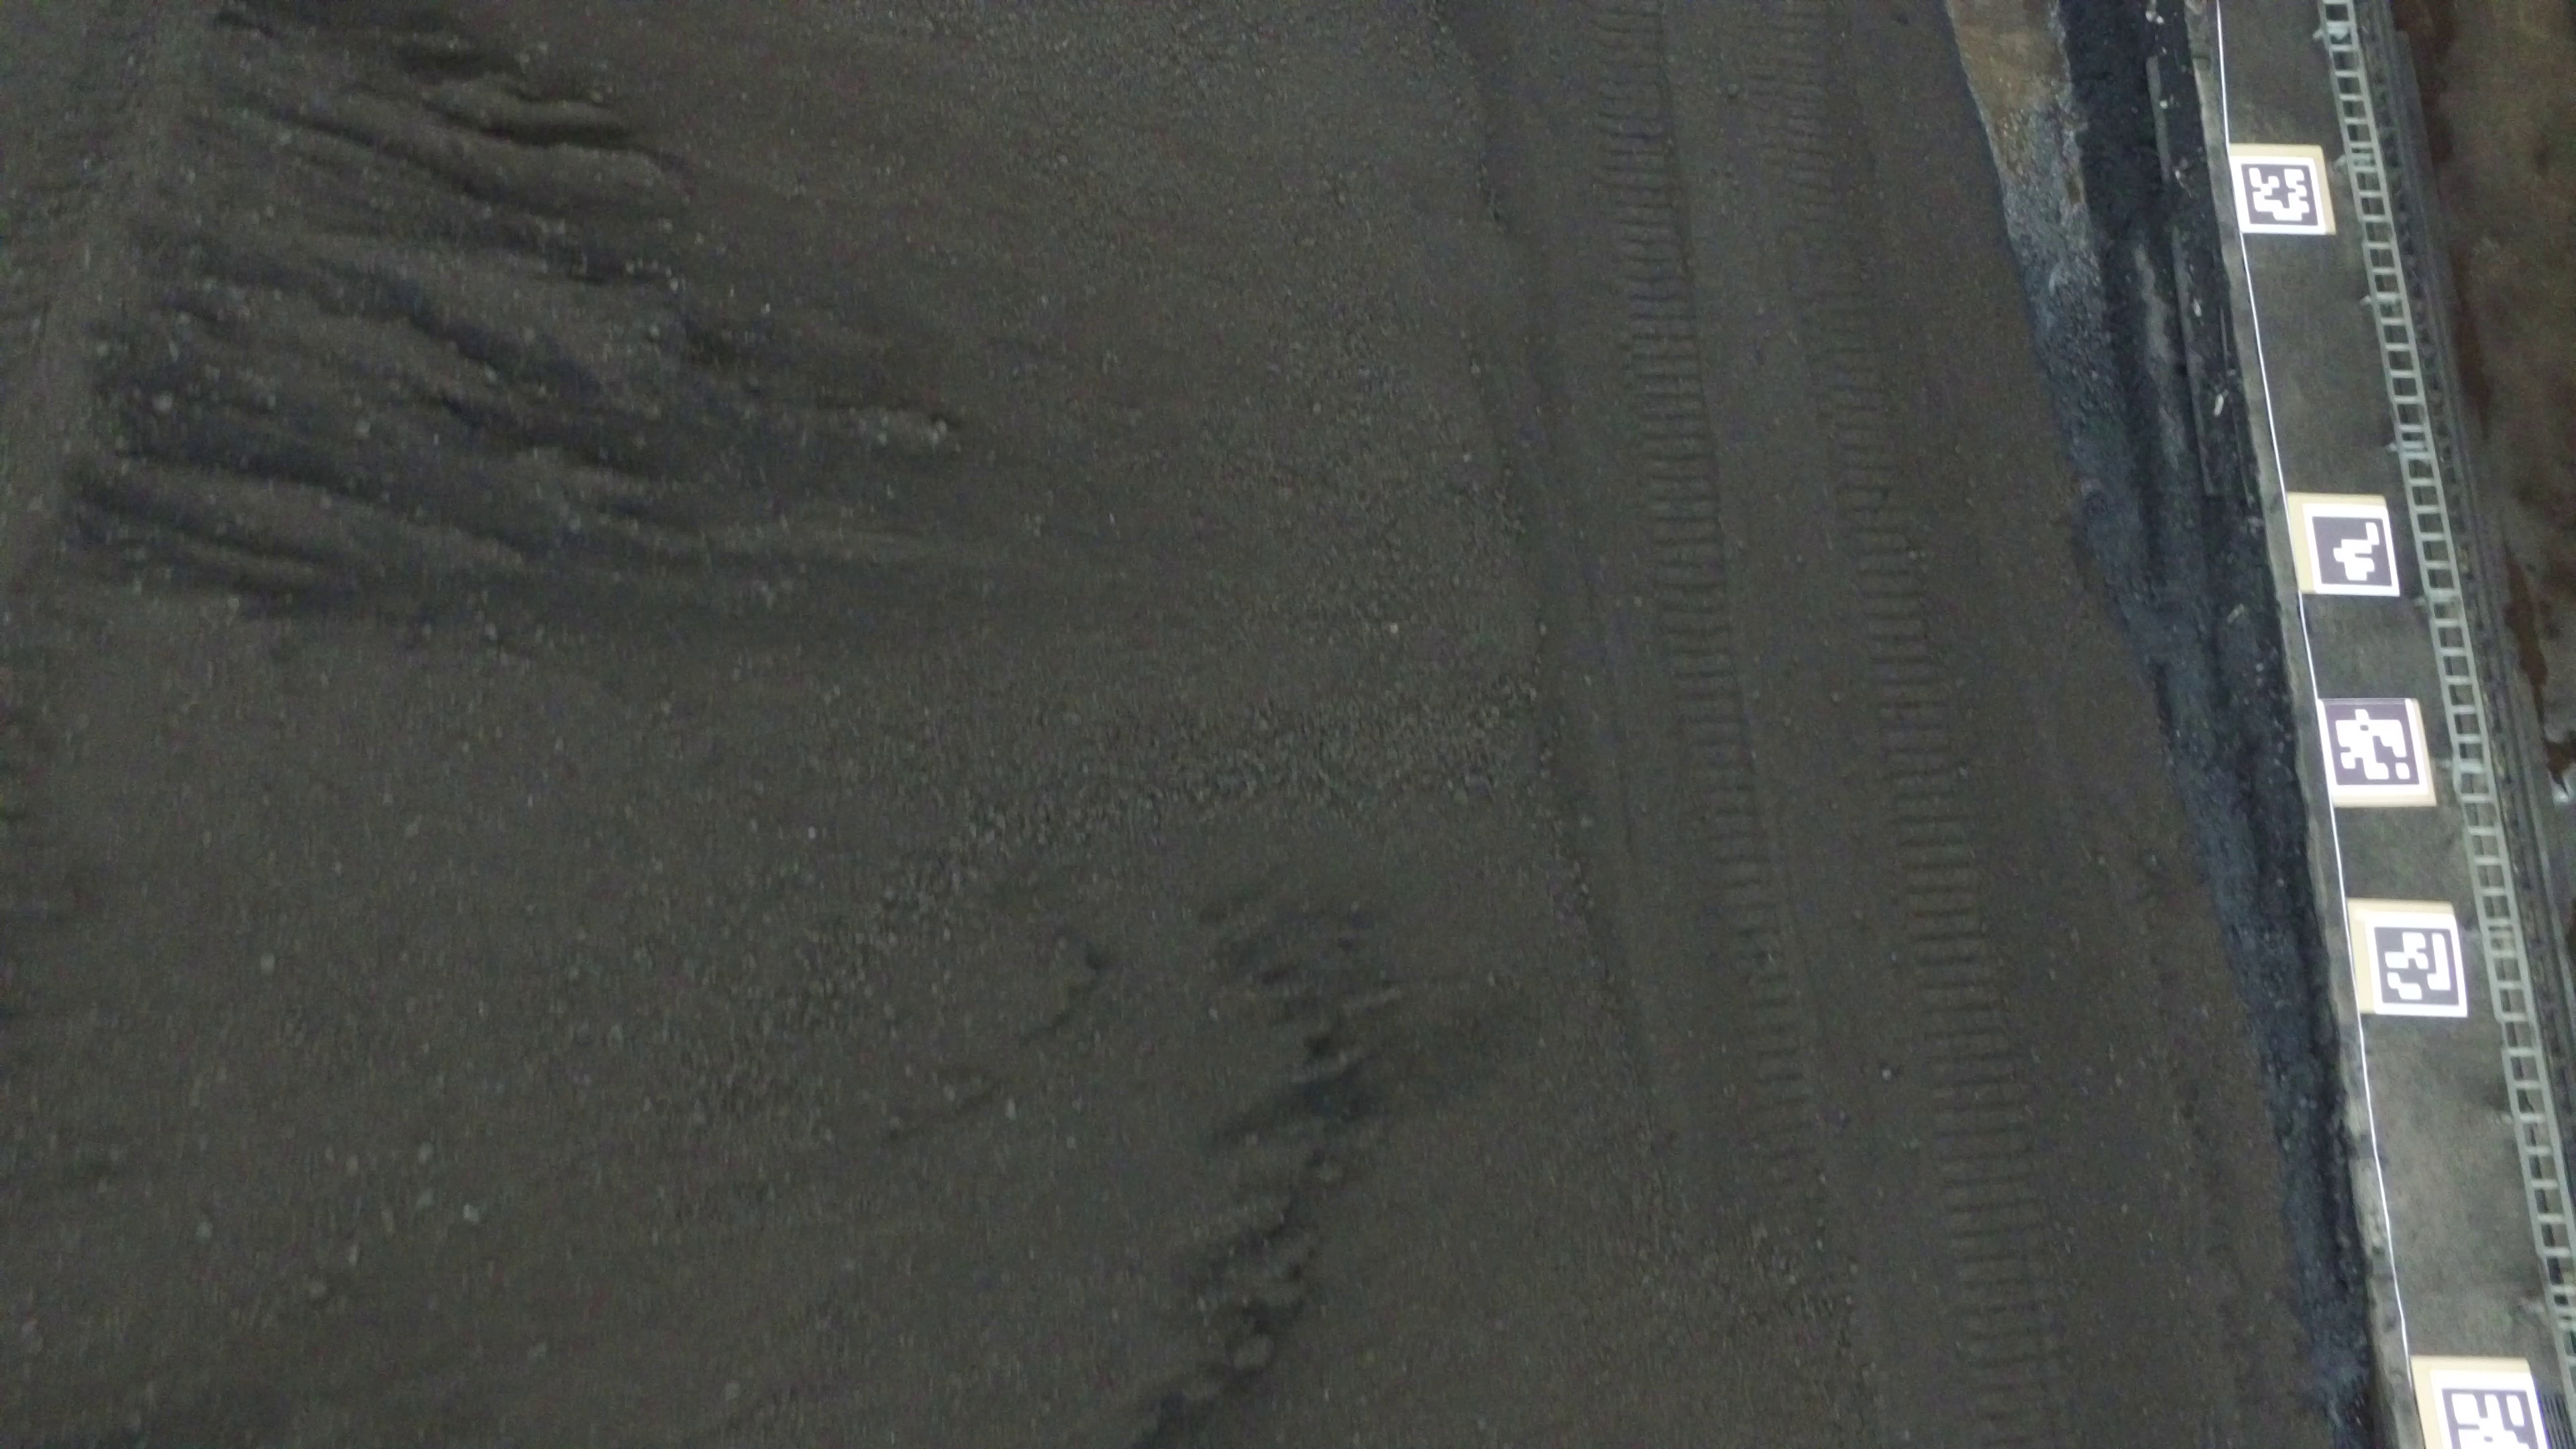
\includegraphics[width=4cm]{2VSLAM_big4.jpg}\hskip1cm}
      \subcaptionbox{Frame5}{\label{fig:2VSLAM_big5}
      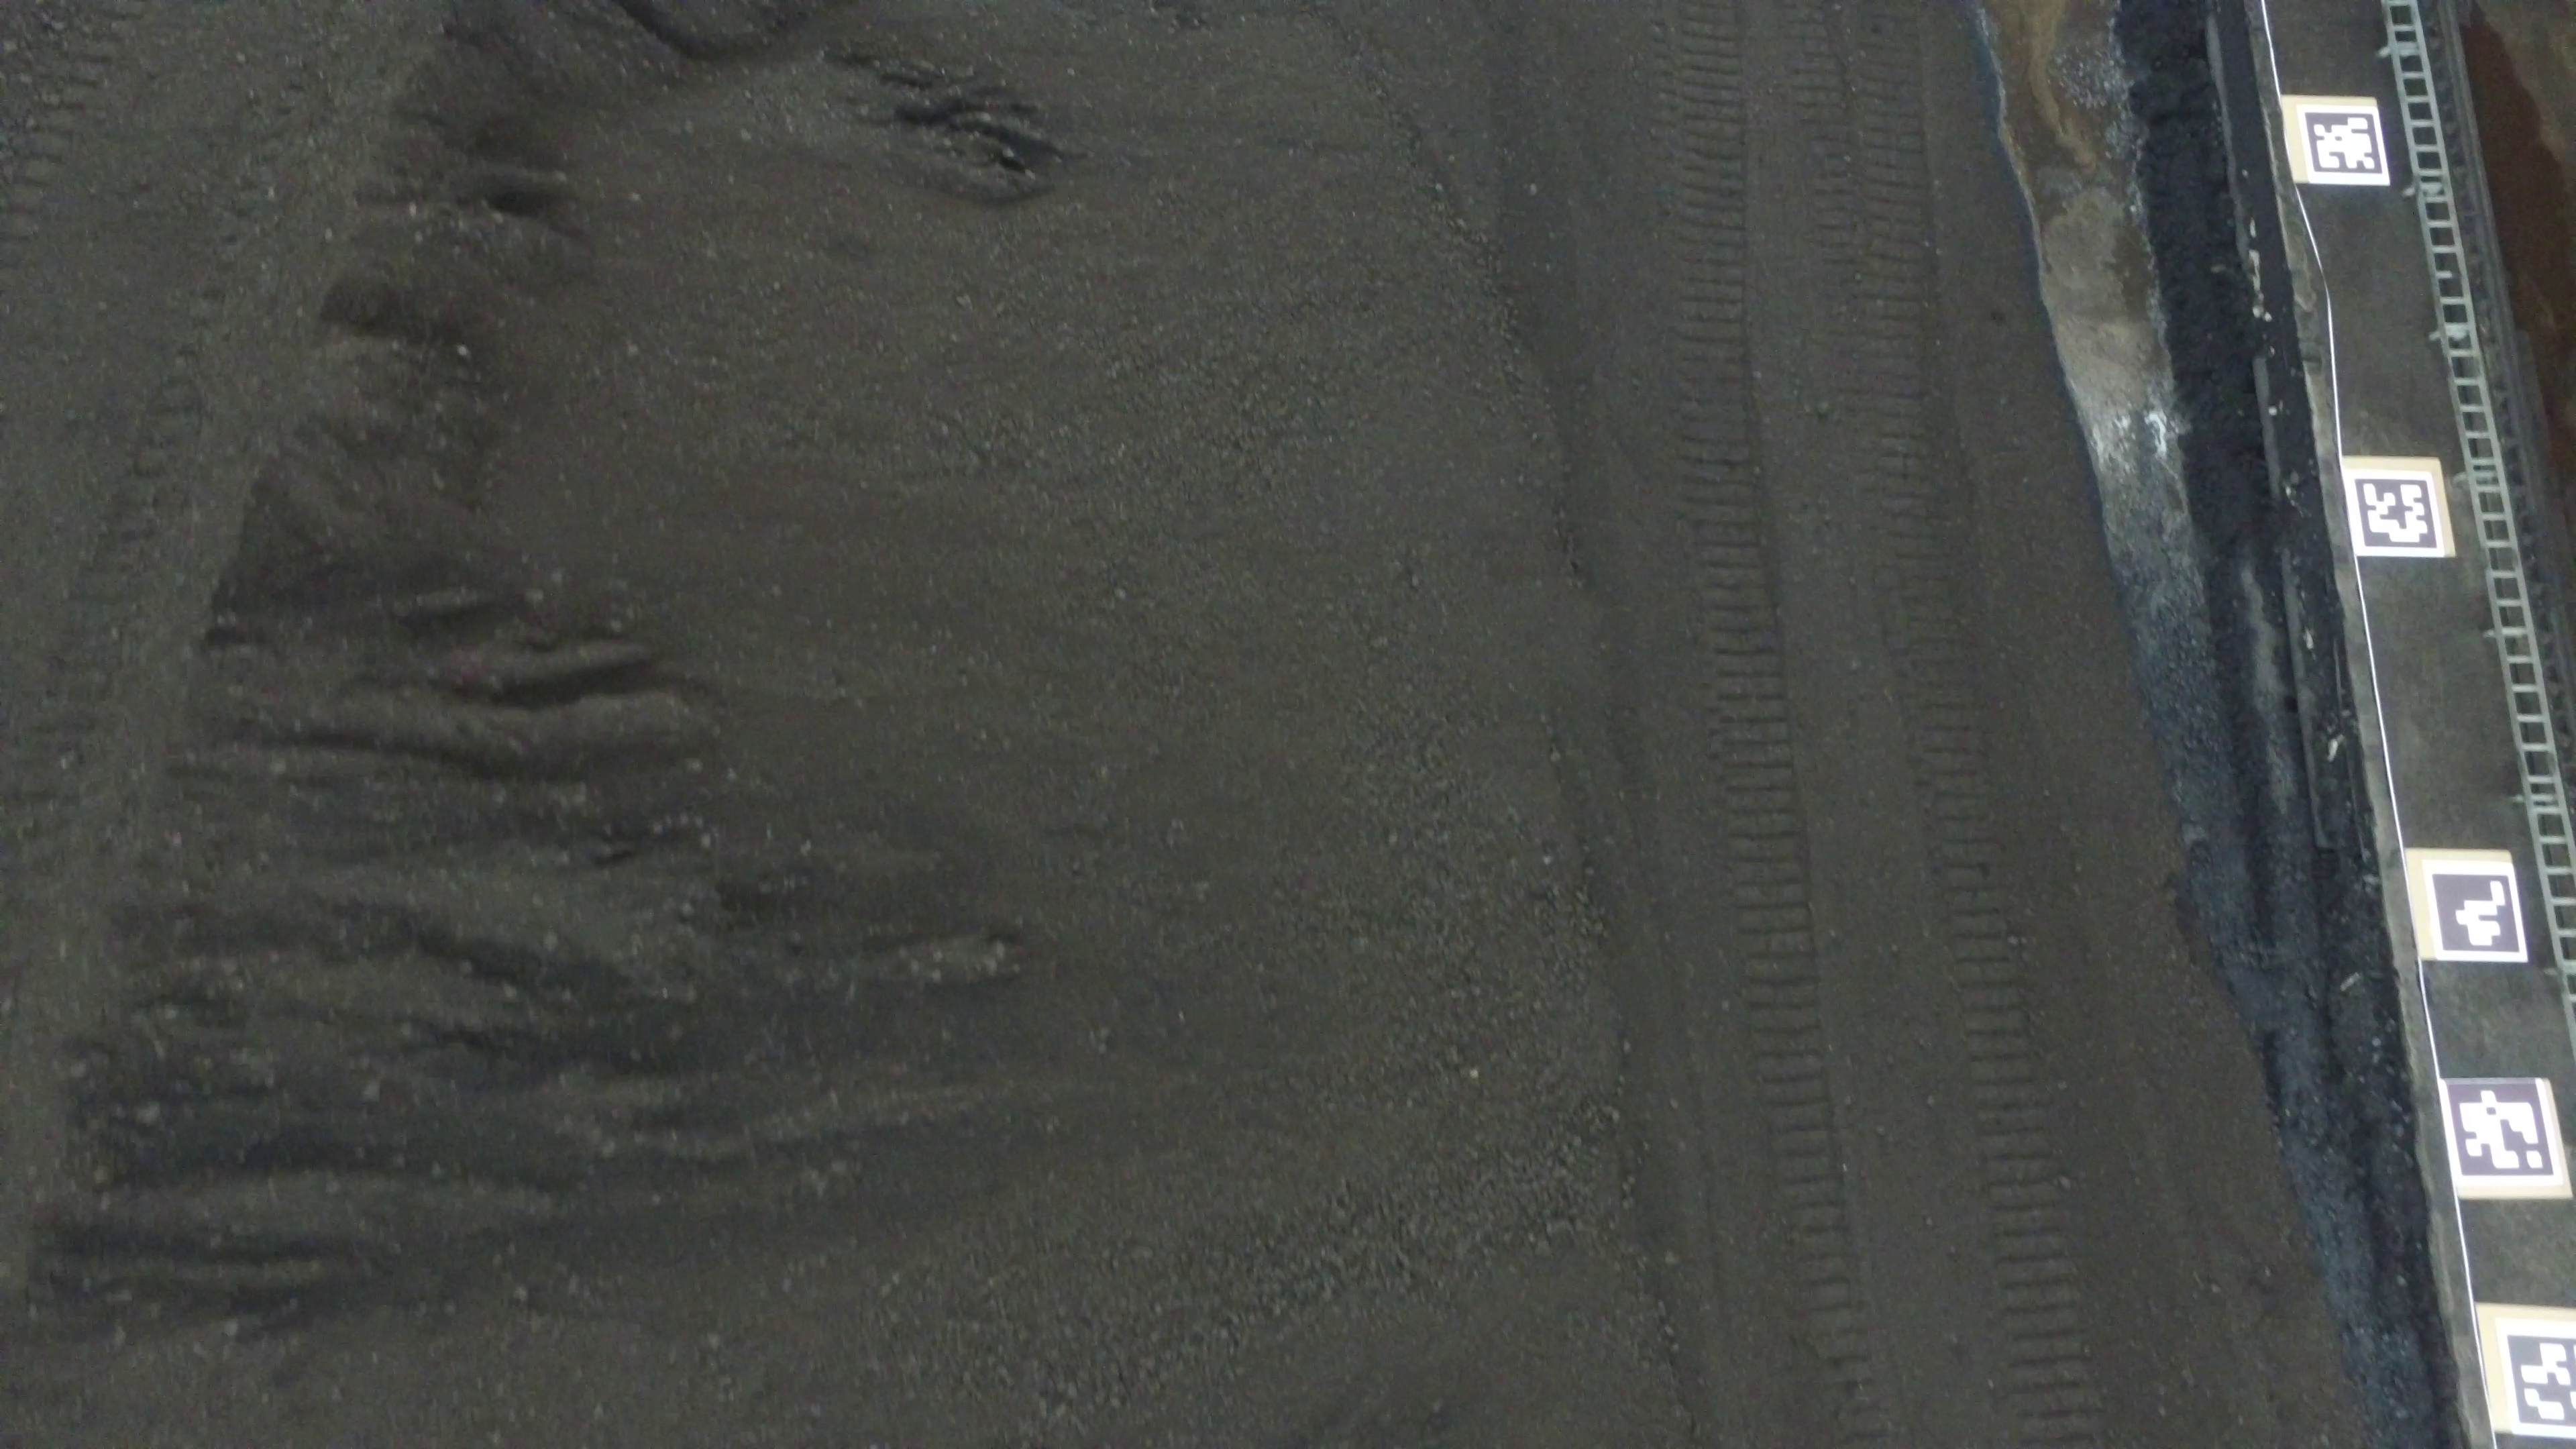
\includegraphics[width=4cm]{2VSLAM_big5.jpg}\hskip1cm}
      \subcaptionbox{Frame6}{\label{fig:2VSLAM_big6}
      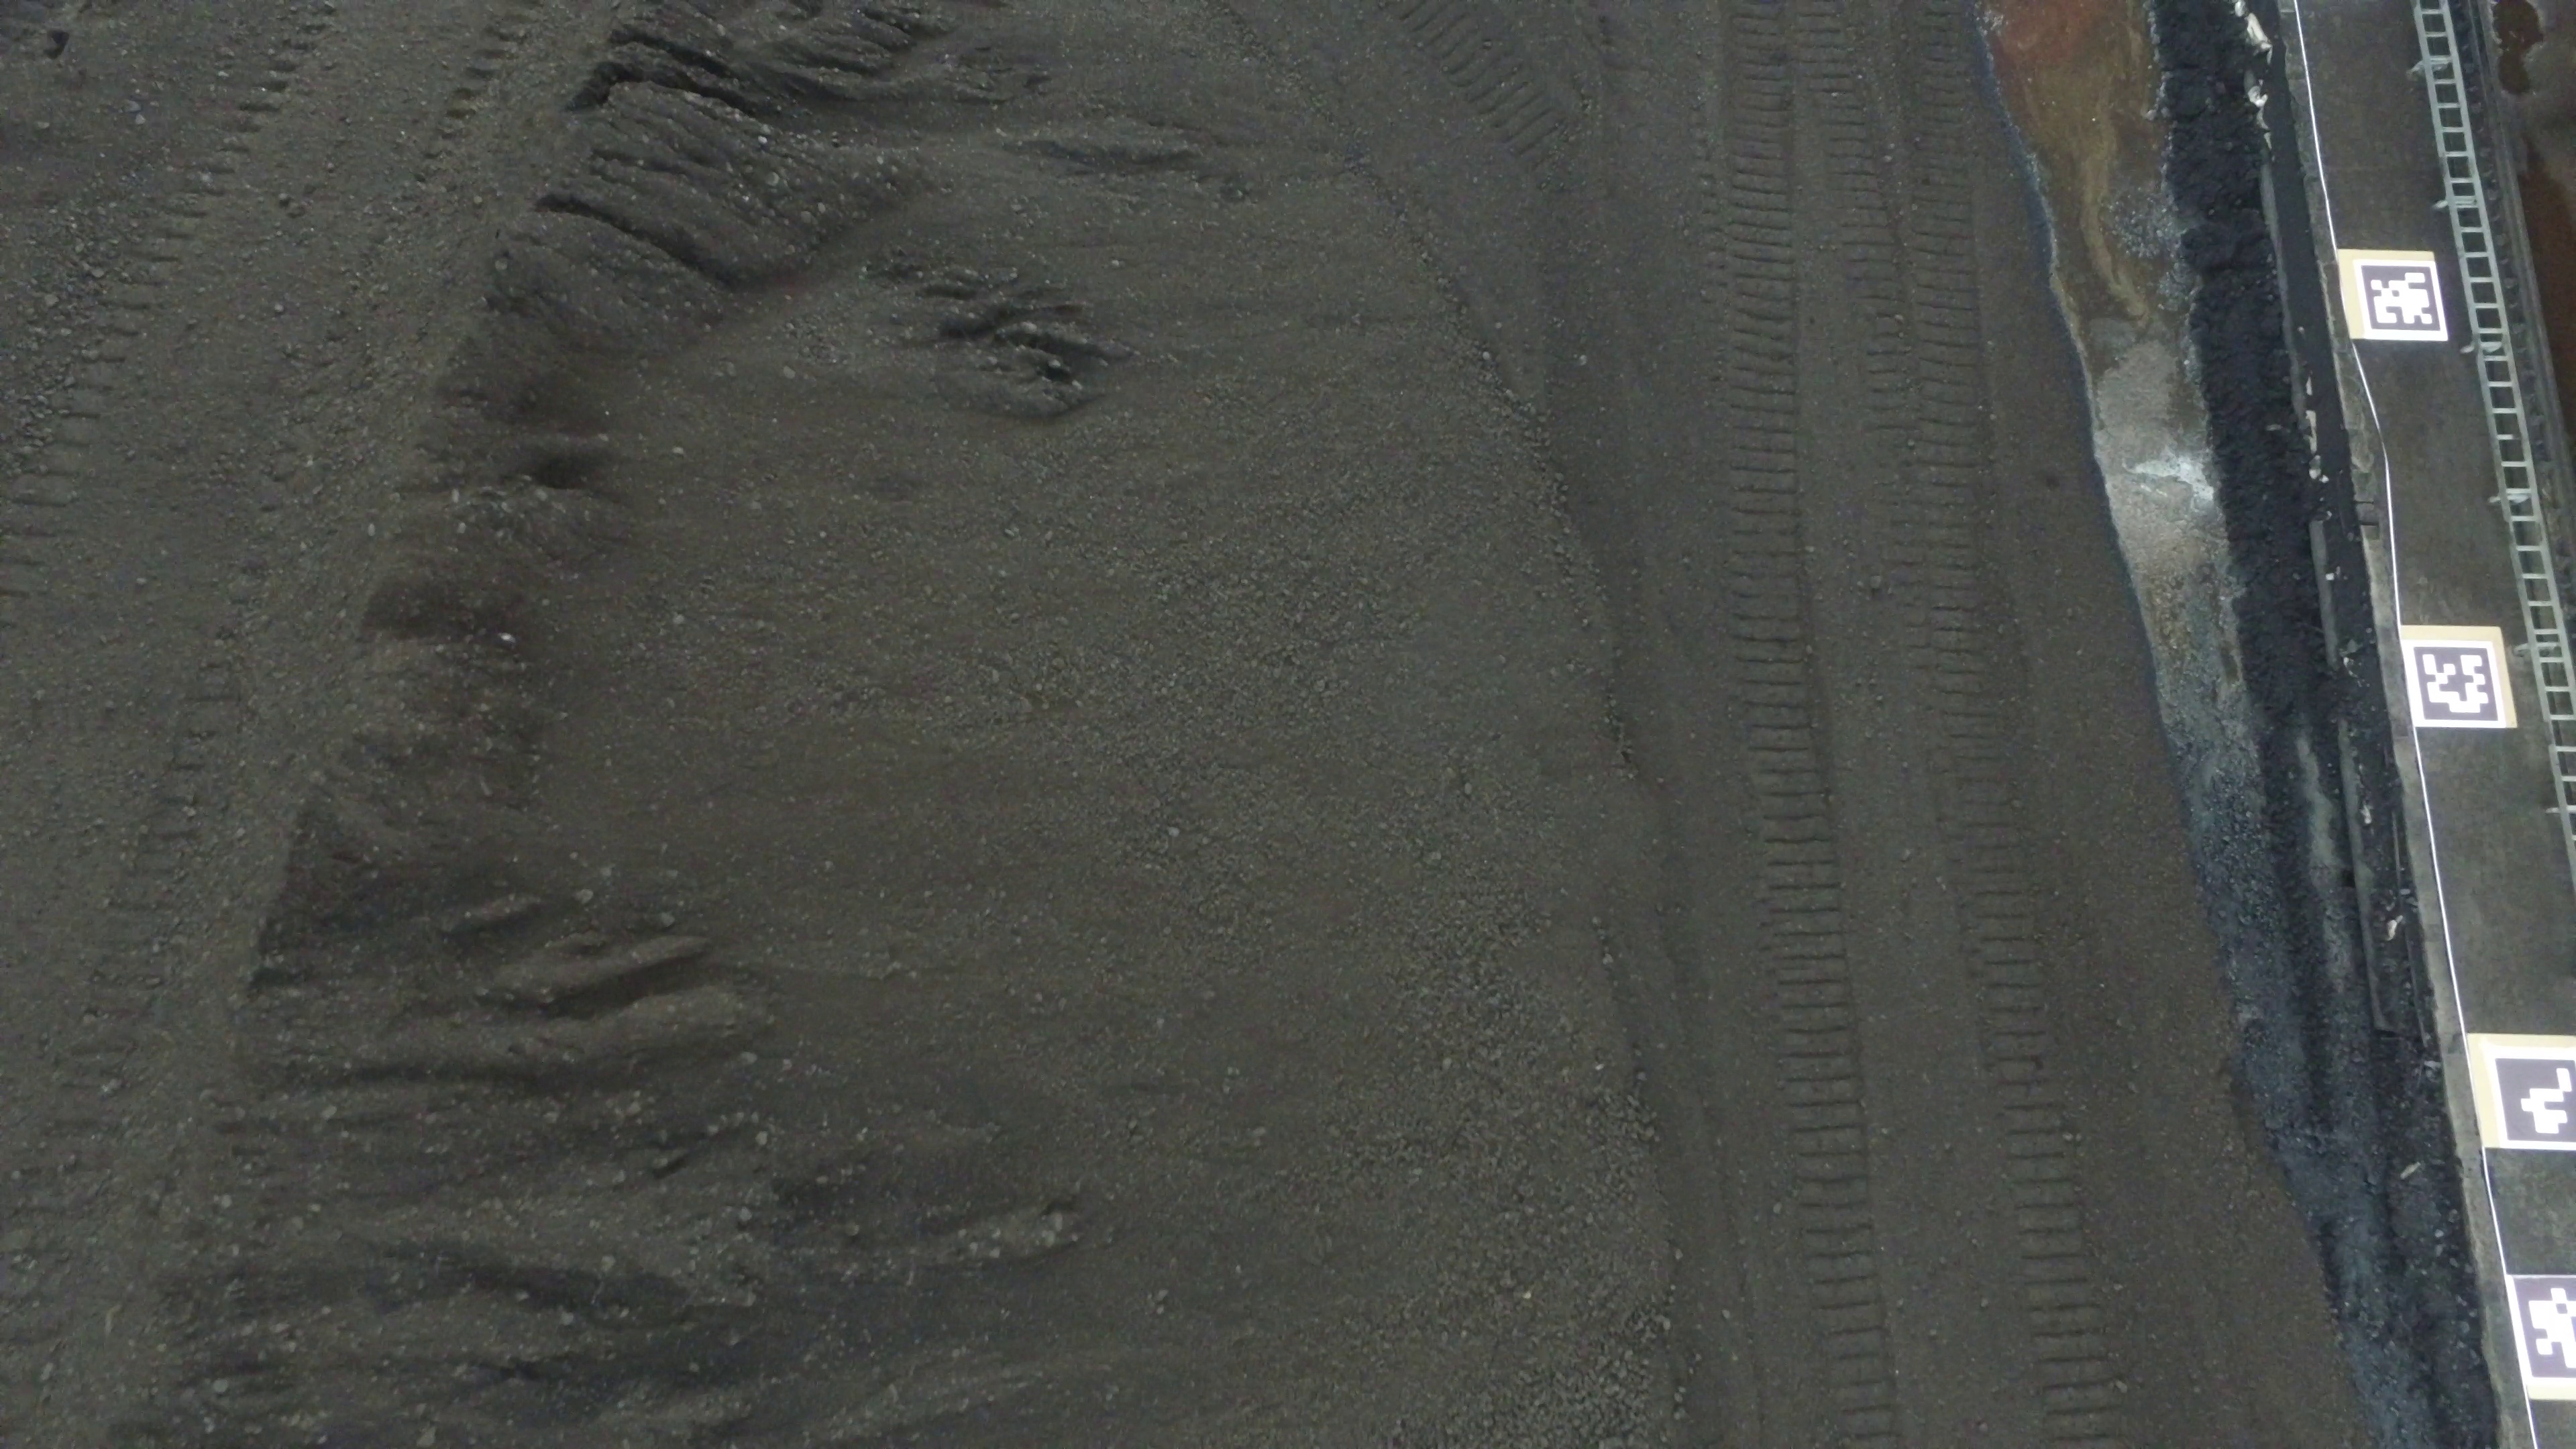
\includegraphics[width=4cm]{2VSLAM_big6.jpg}}
    \vskip0.2cm      
      \subcaptionbox{Frame7}{\label{fig:2VSLAM_big7}
      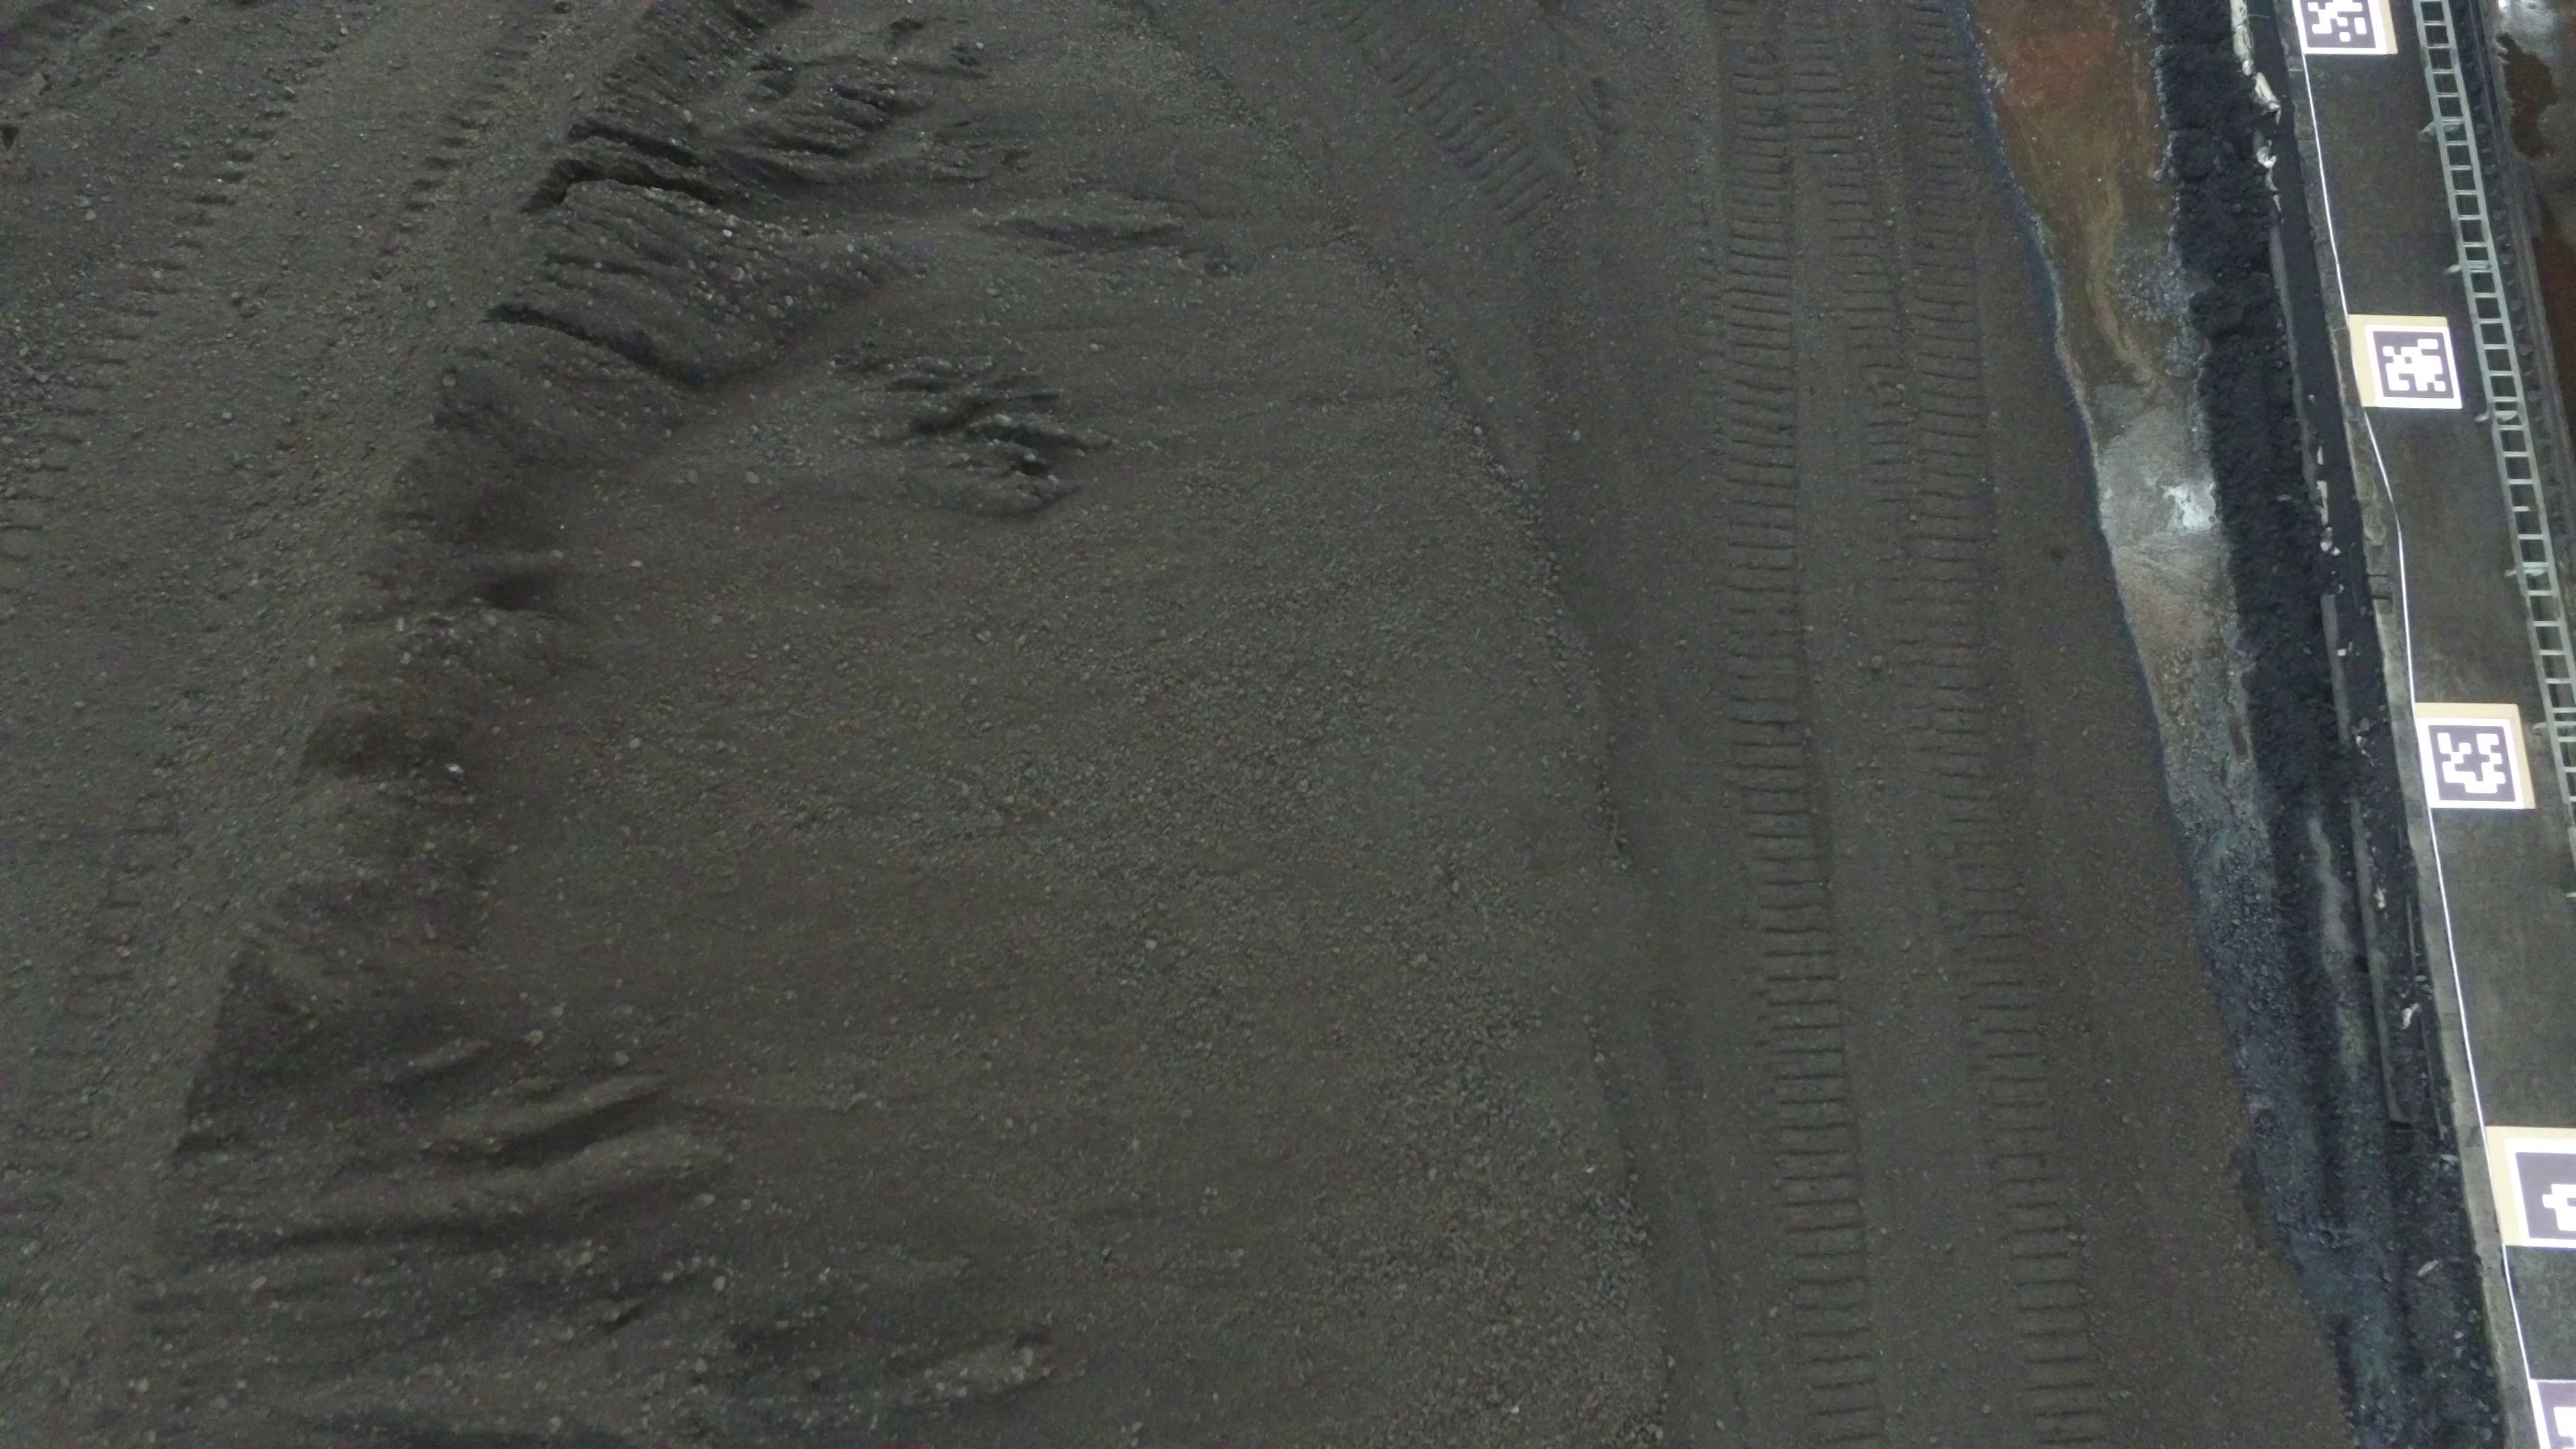
\includegraphics[width=4cm]{2VSLAM_big7.jpg}\hskip1cm}
      \subcaptionbox{Frame8}{\label{fig:2VSLAM_big8}
      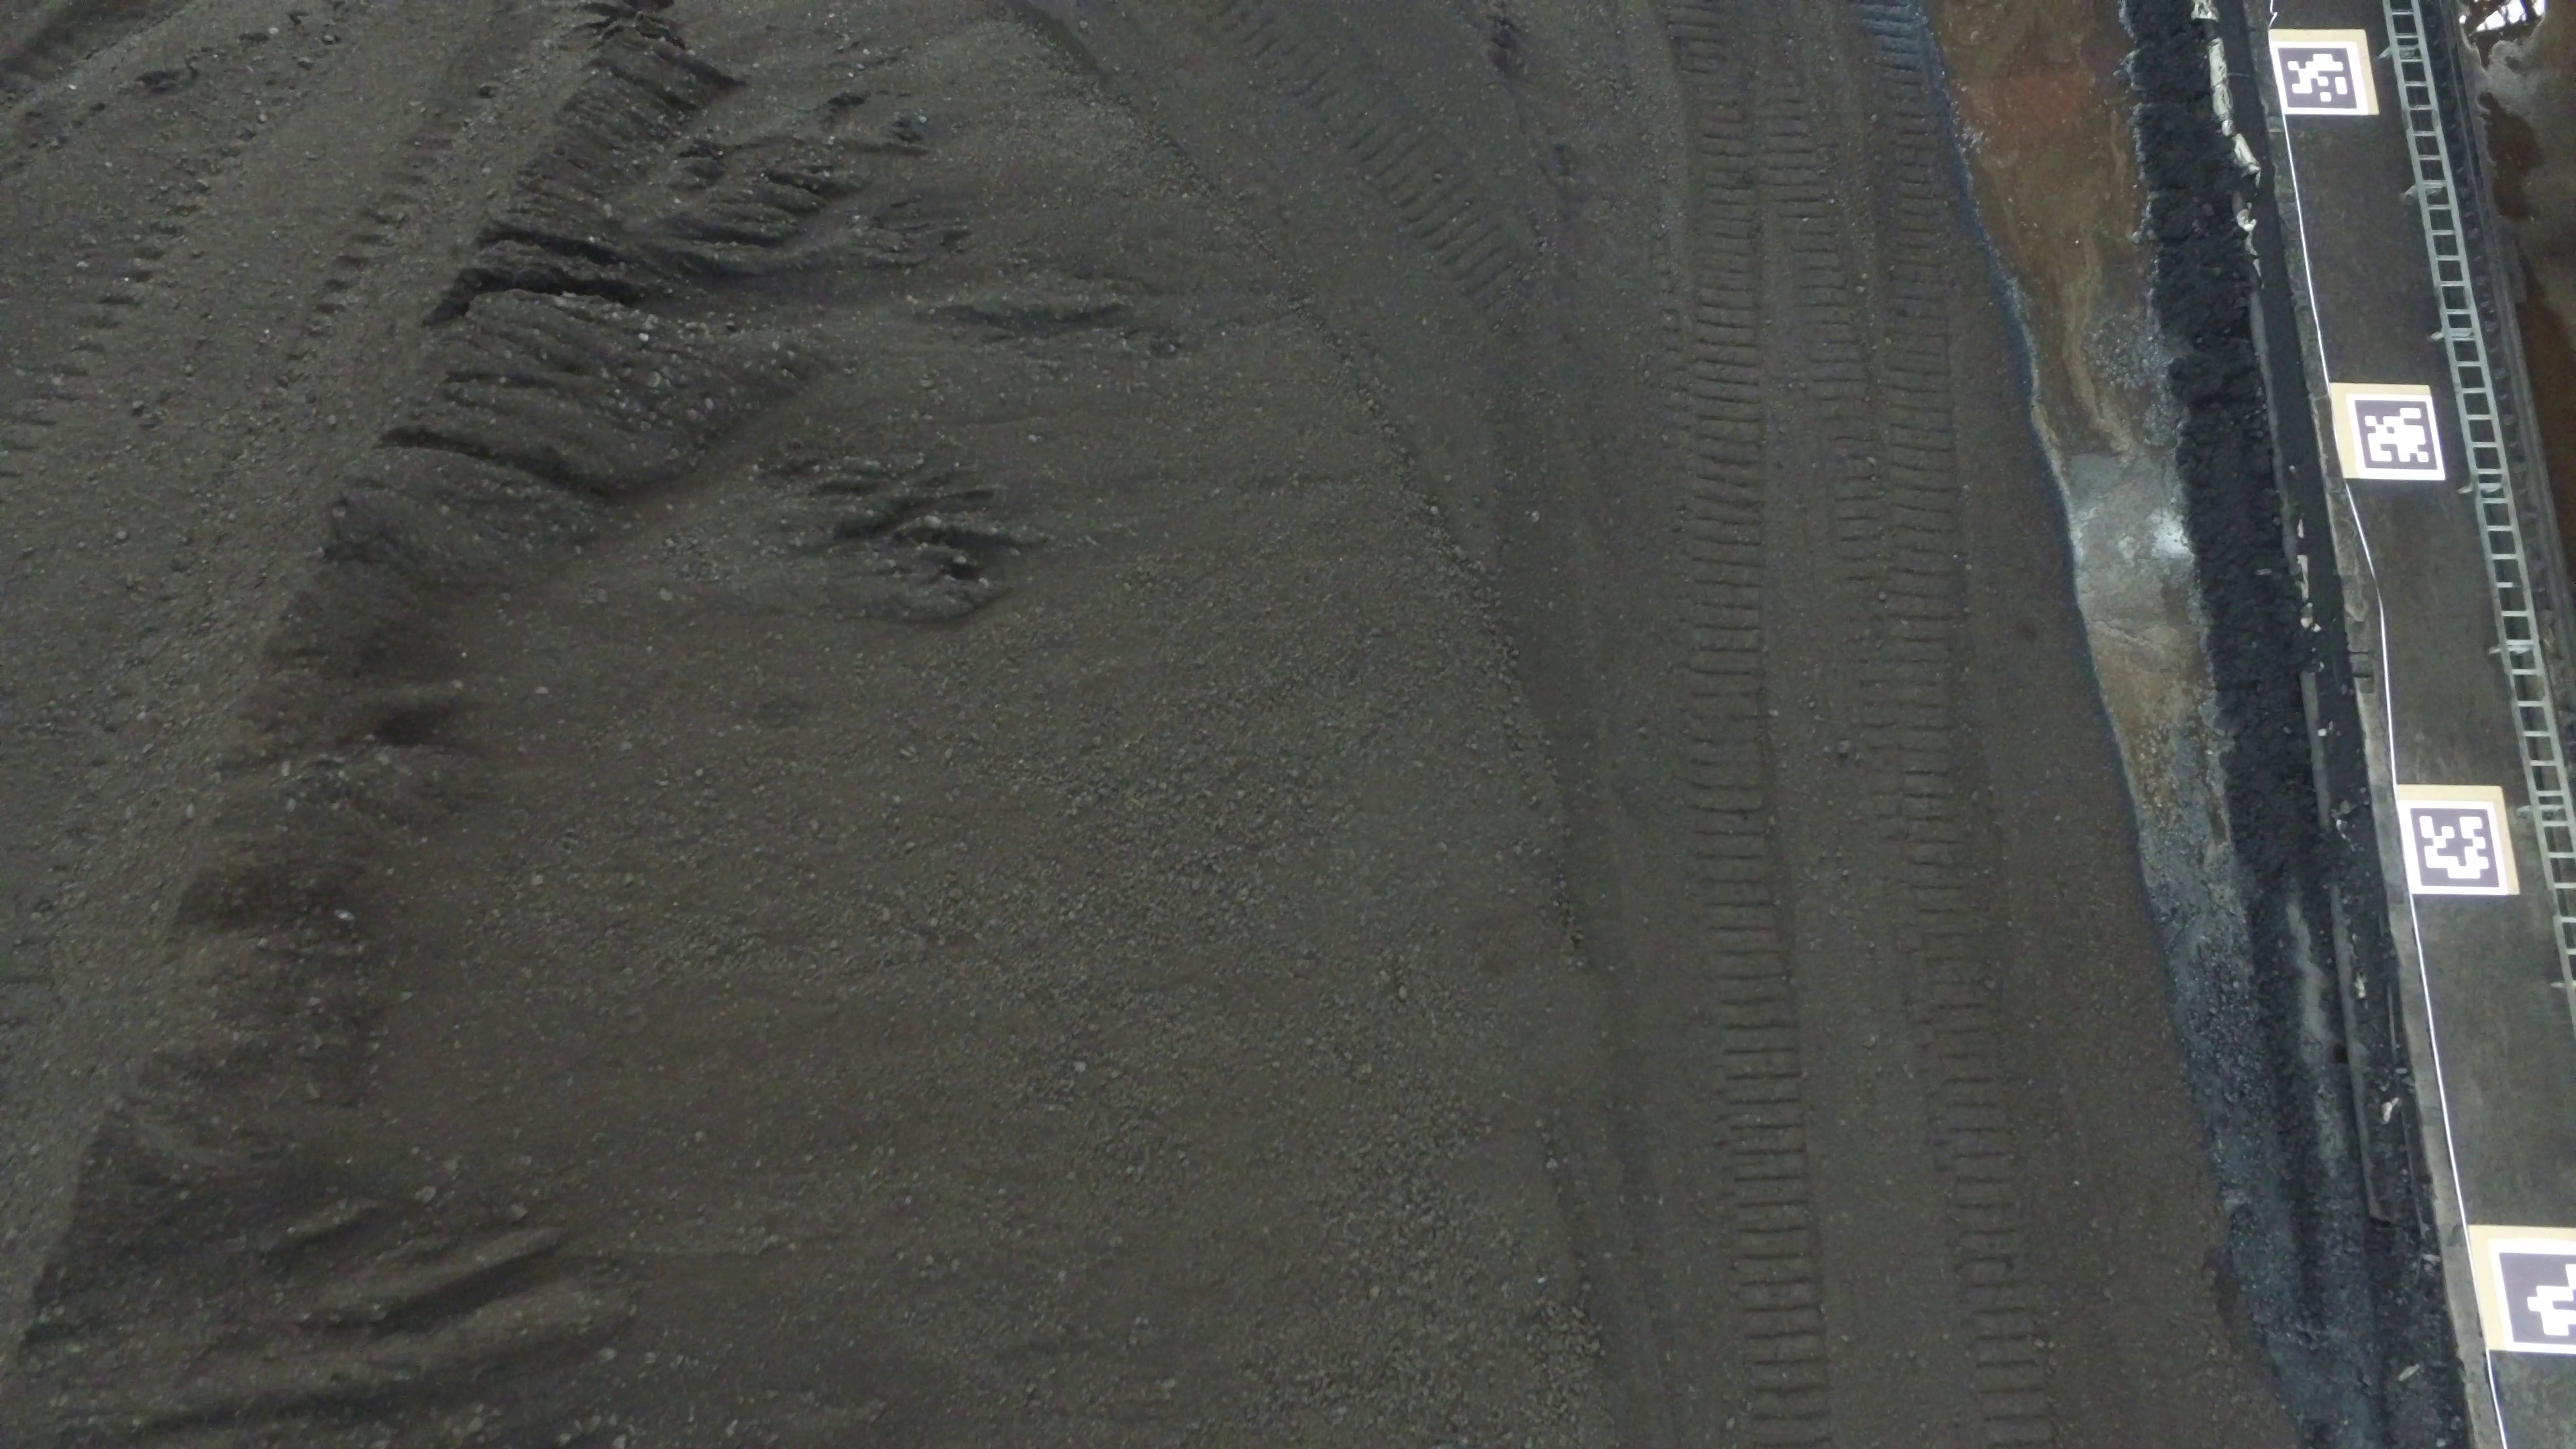
\includegraphics[width=4cm]{2VSLAM_big8.jpg}\hskip1cm}
      \subcaptionbox{Frame9}{\label{fig:2VSLAM_big9}
      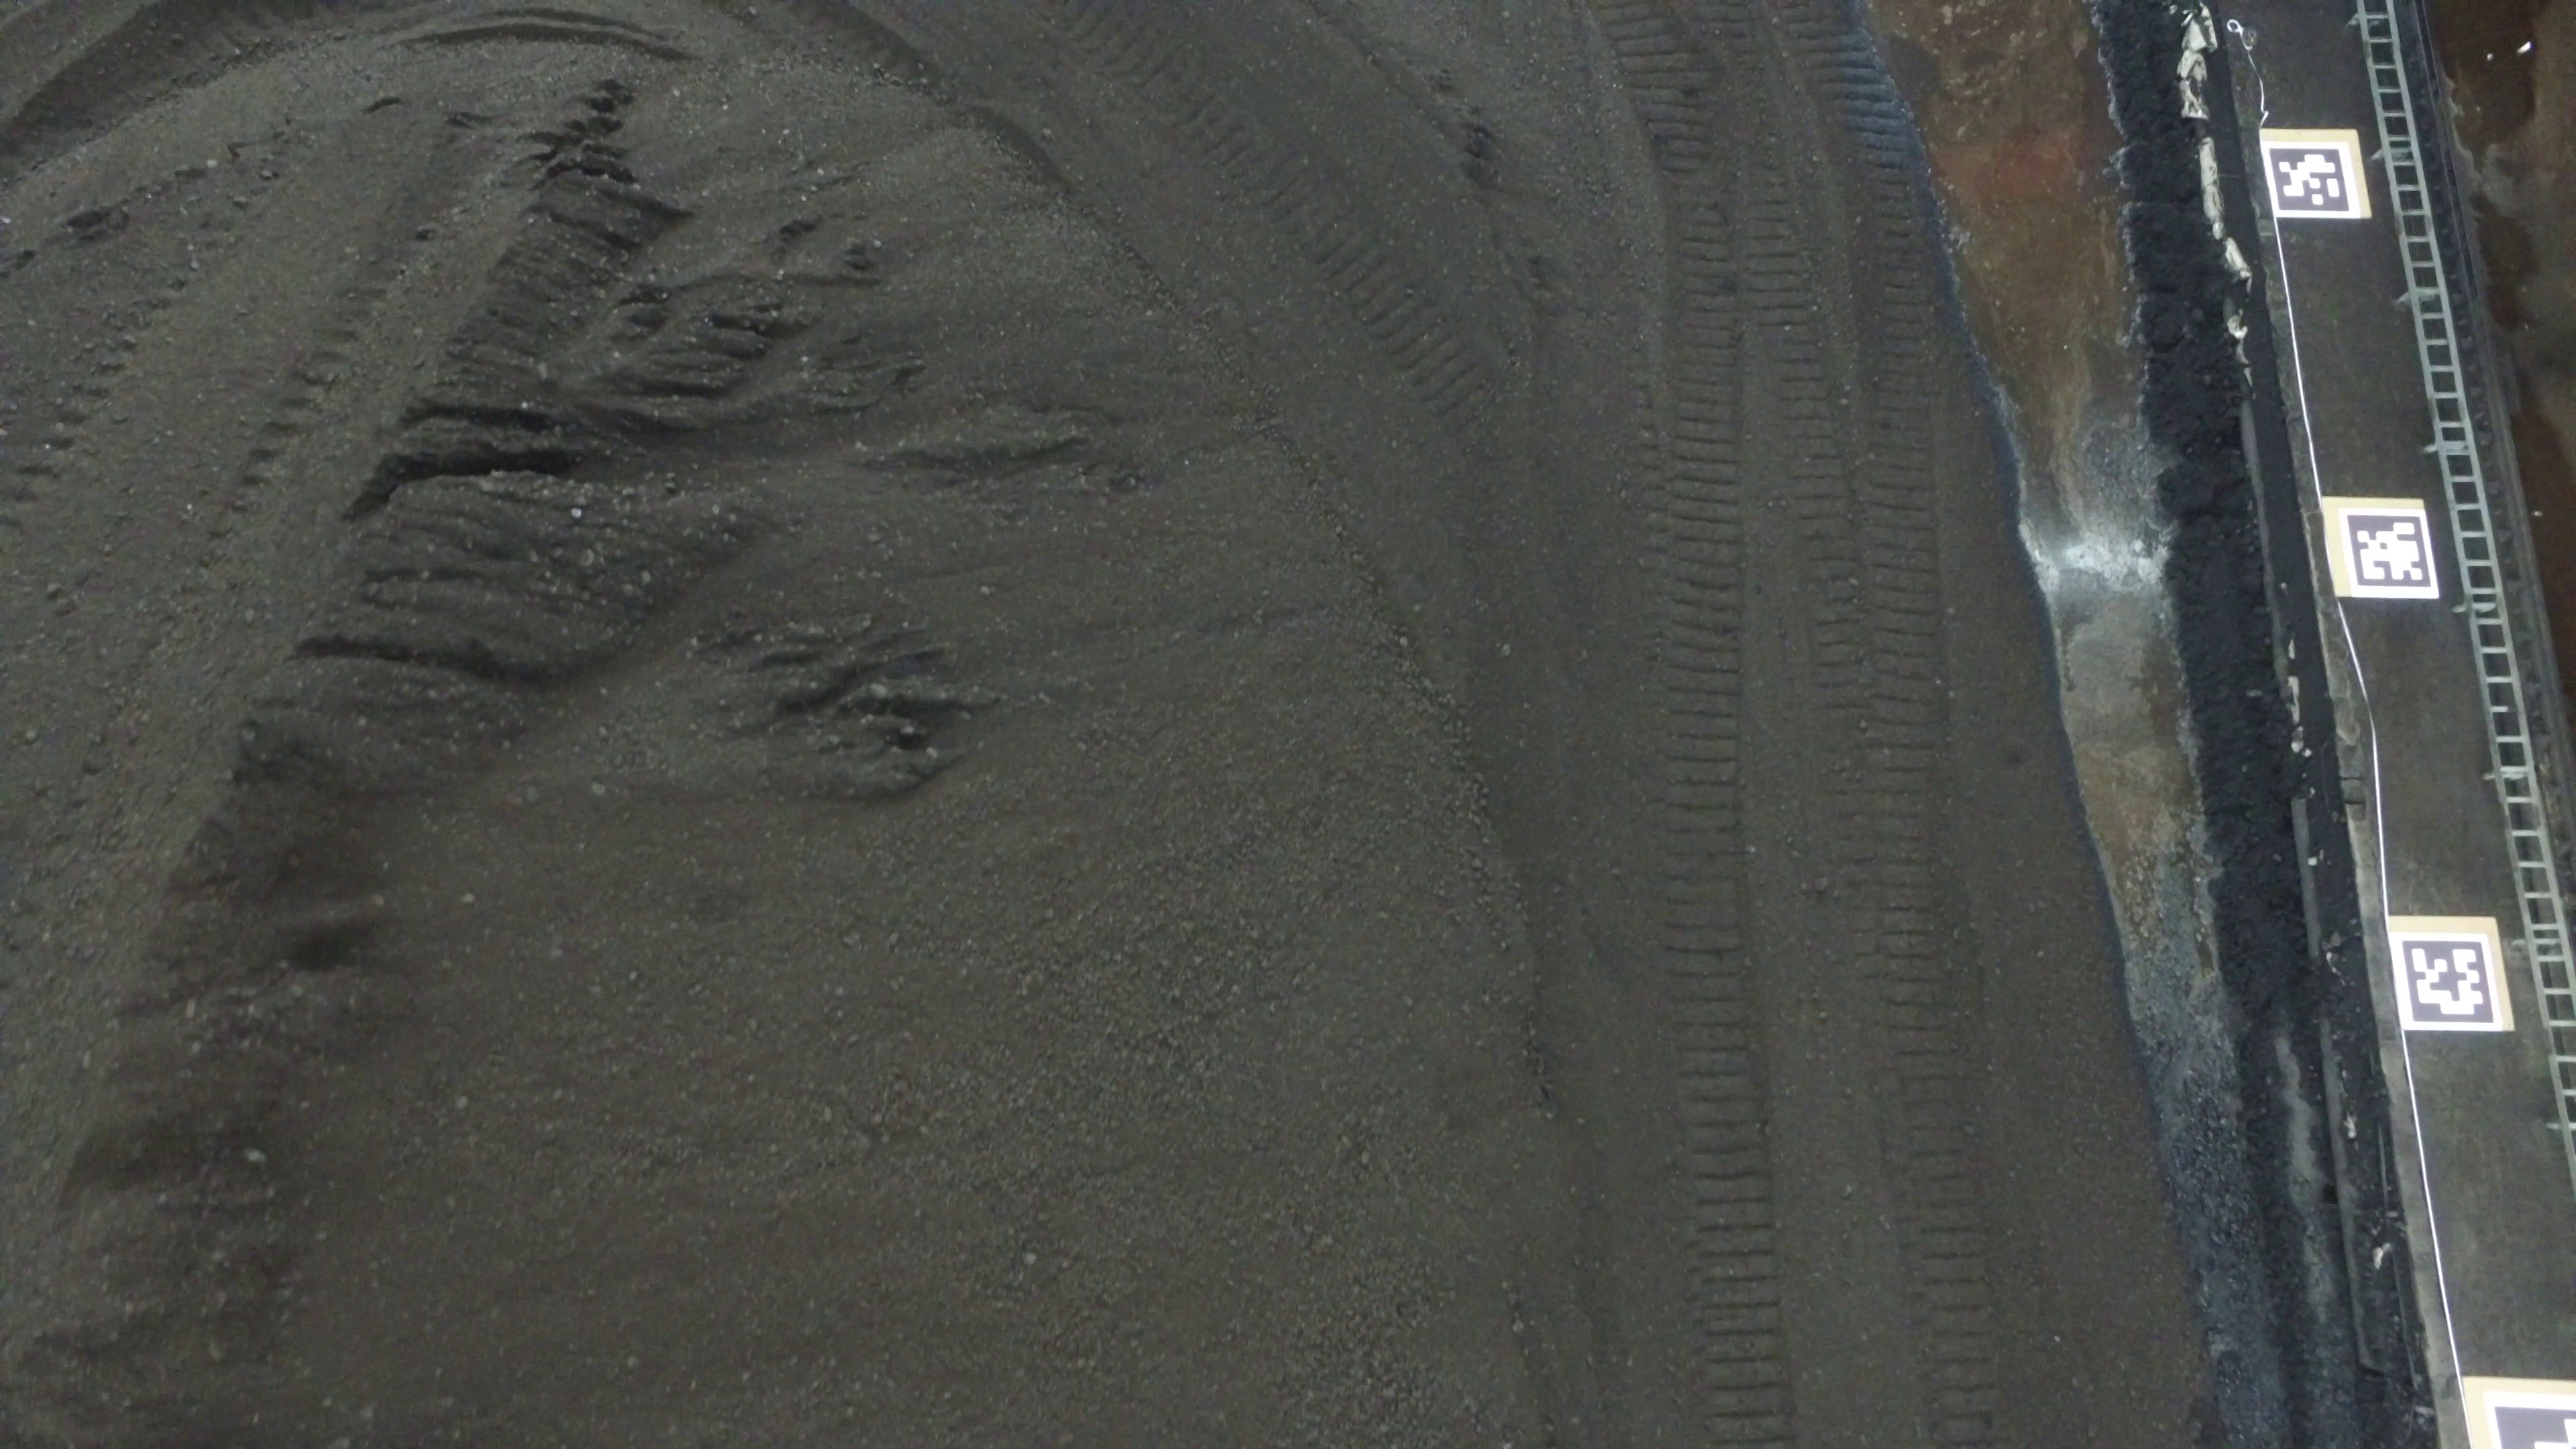
\includegraphics[width=4cm]{2VSLAM_big9.jpg}}
  \vskip0.2cm
    \subcaptionbox{Frame10}{\label{fig:2VSLAM_big10}
    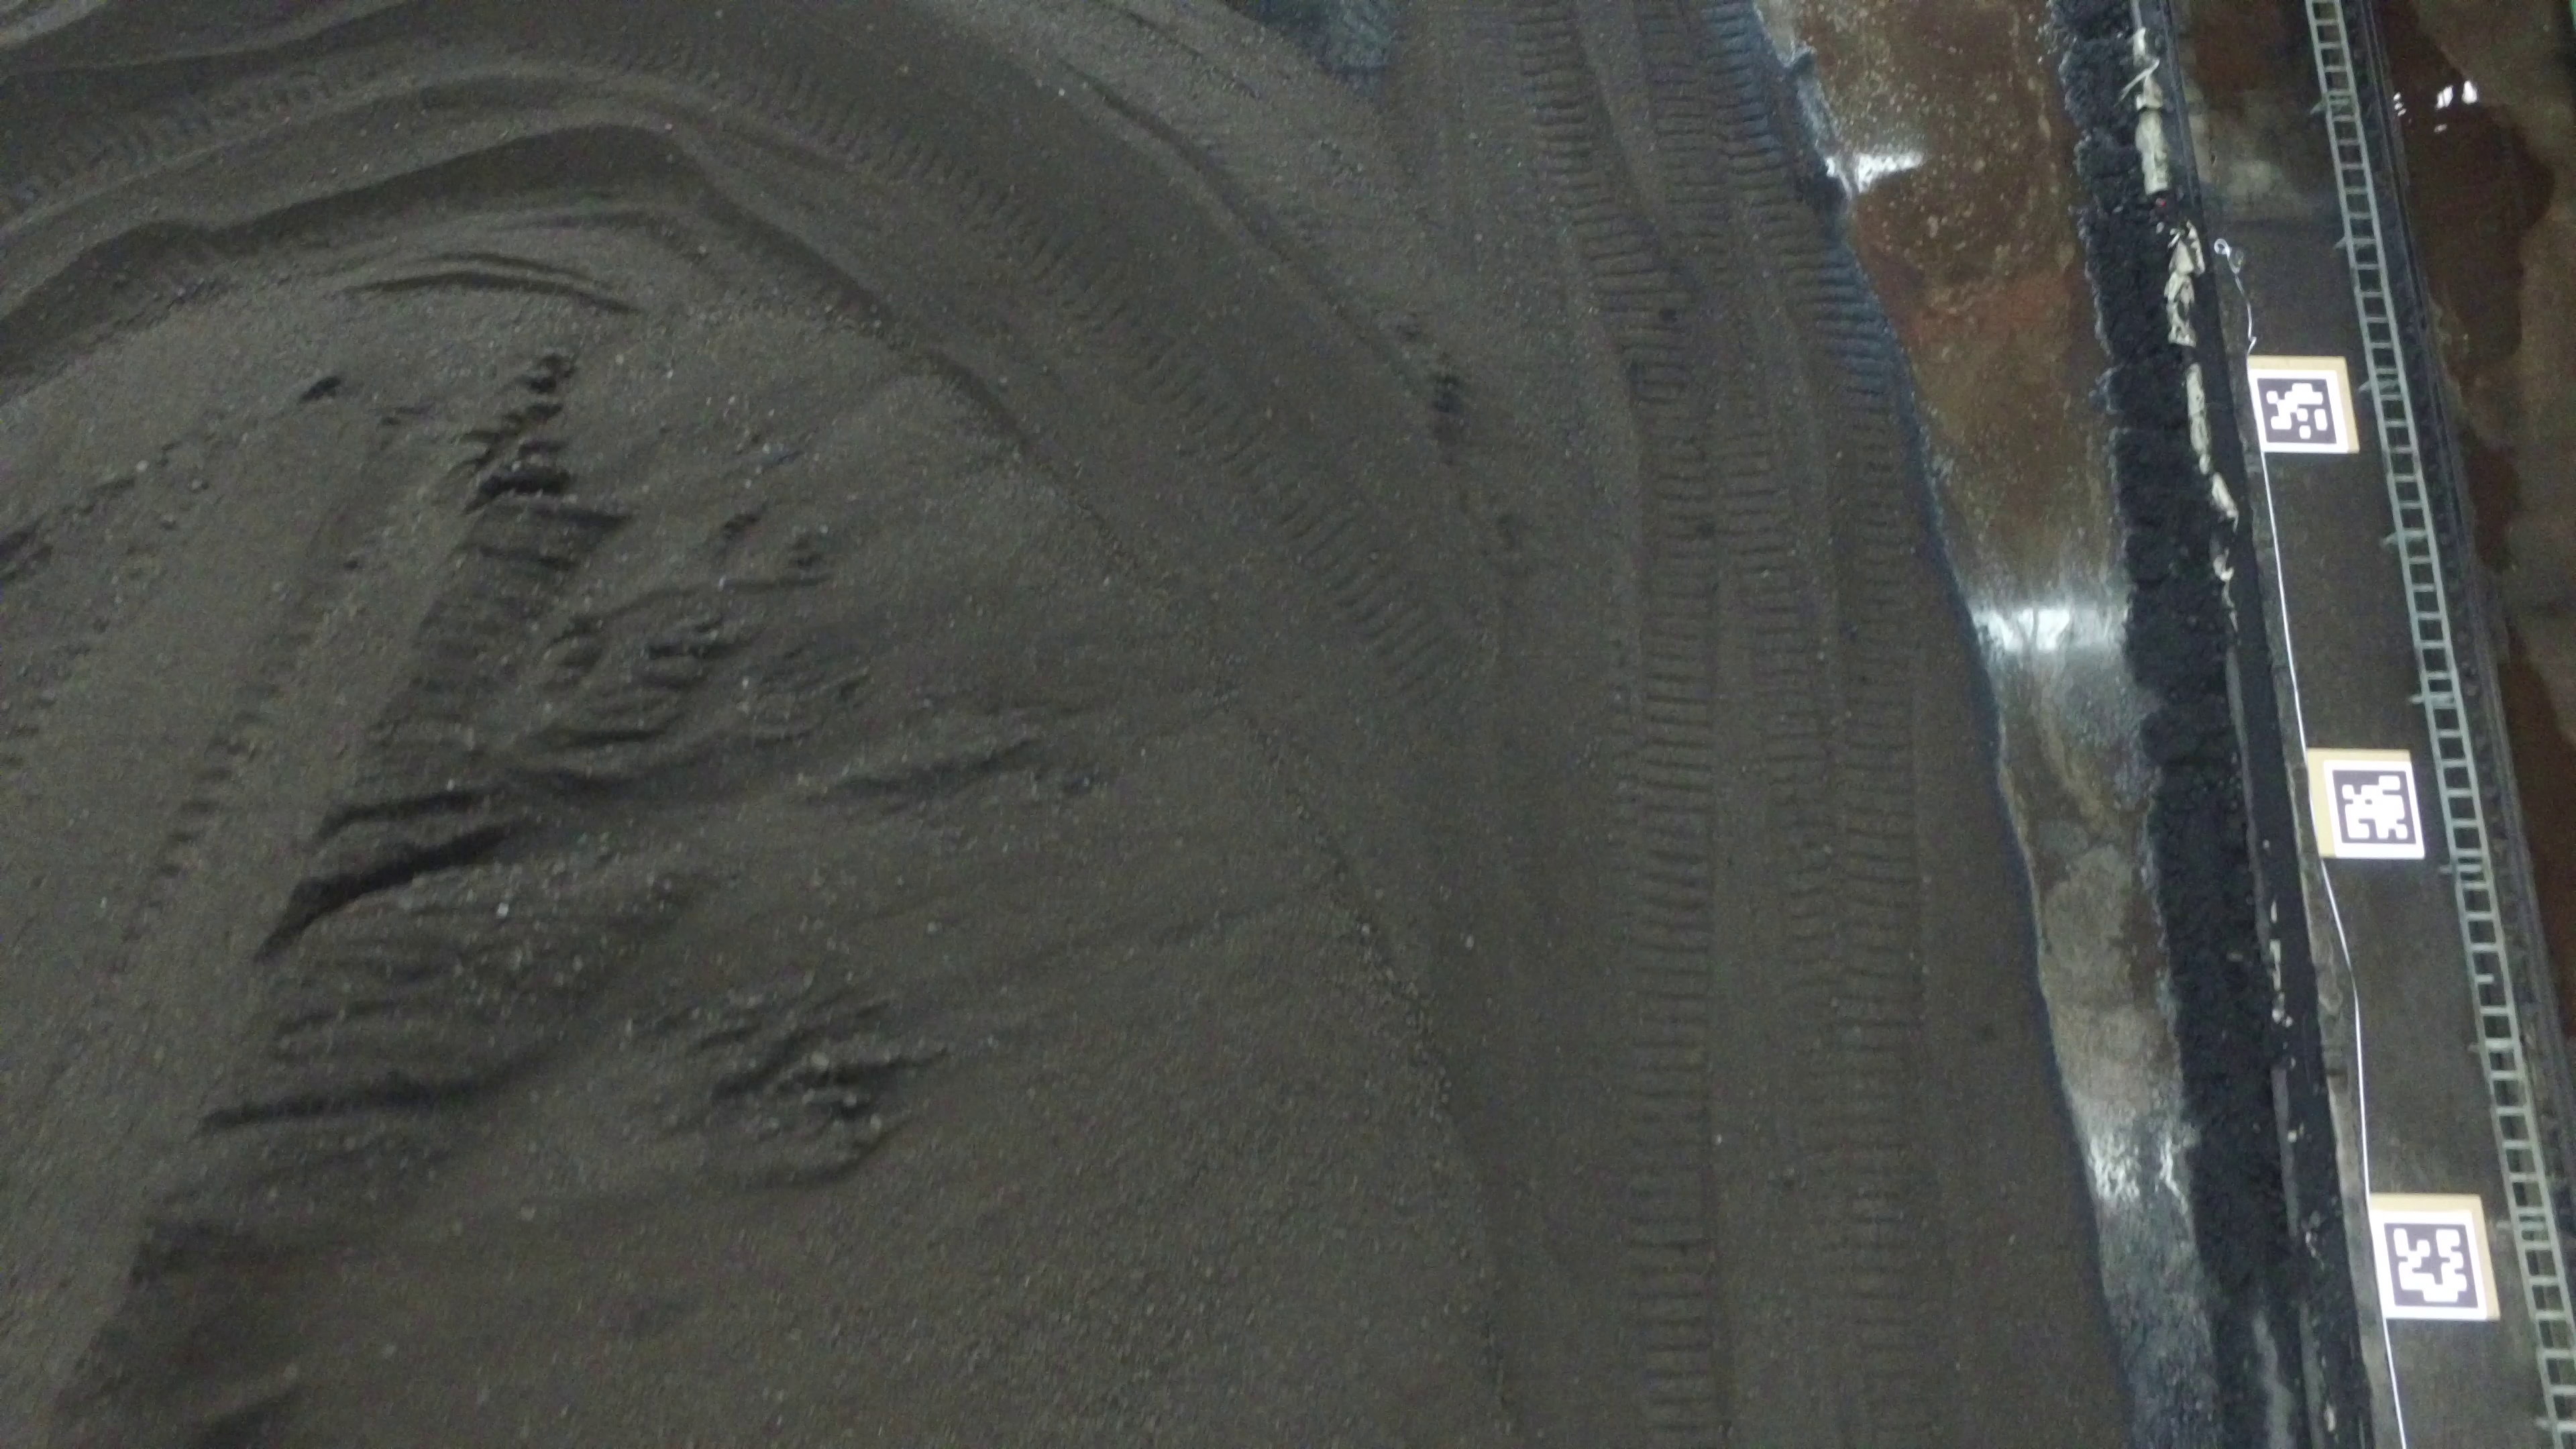
\includegraphics[width=4cm]{2VSLAM_big10.jpg}\hskip1cm}
    \subcaptionbox{Frame11}{\label{fig:2VSLAM_big11}
    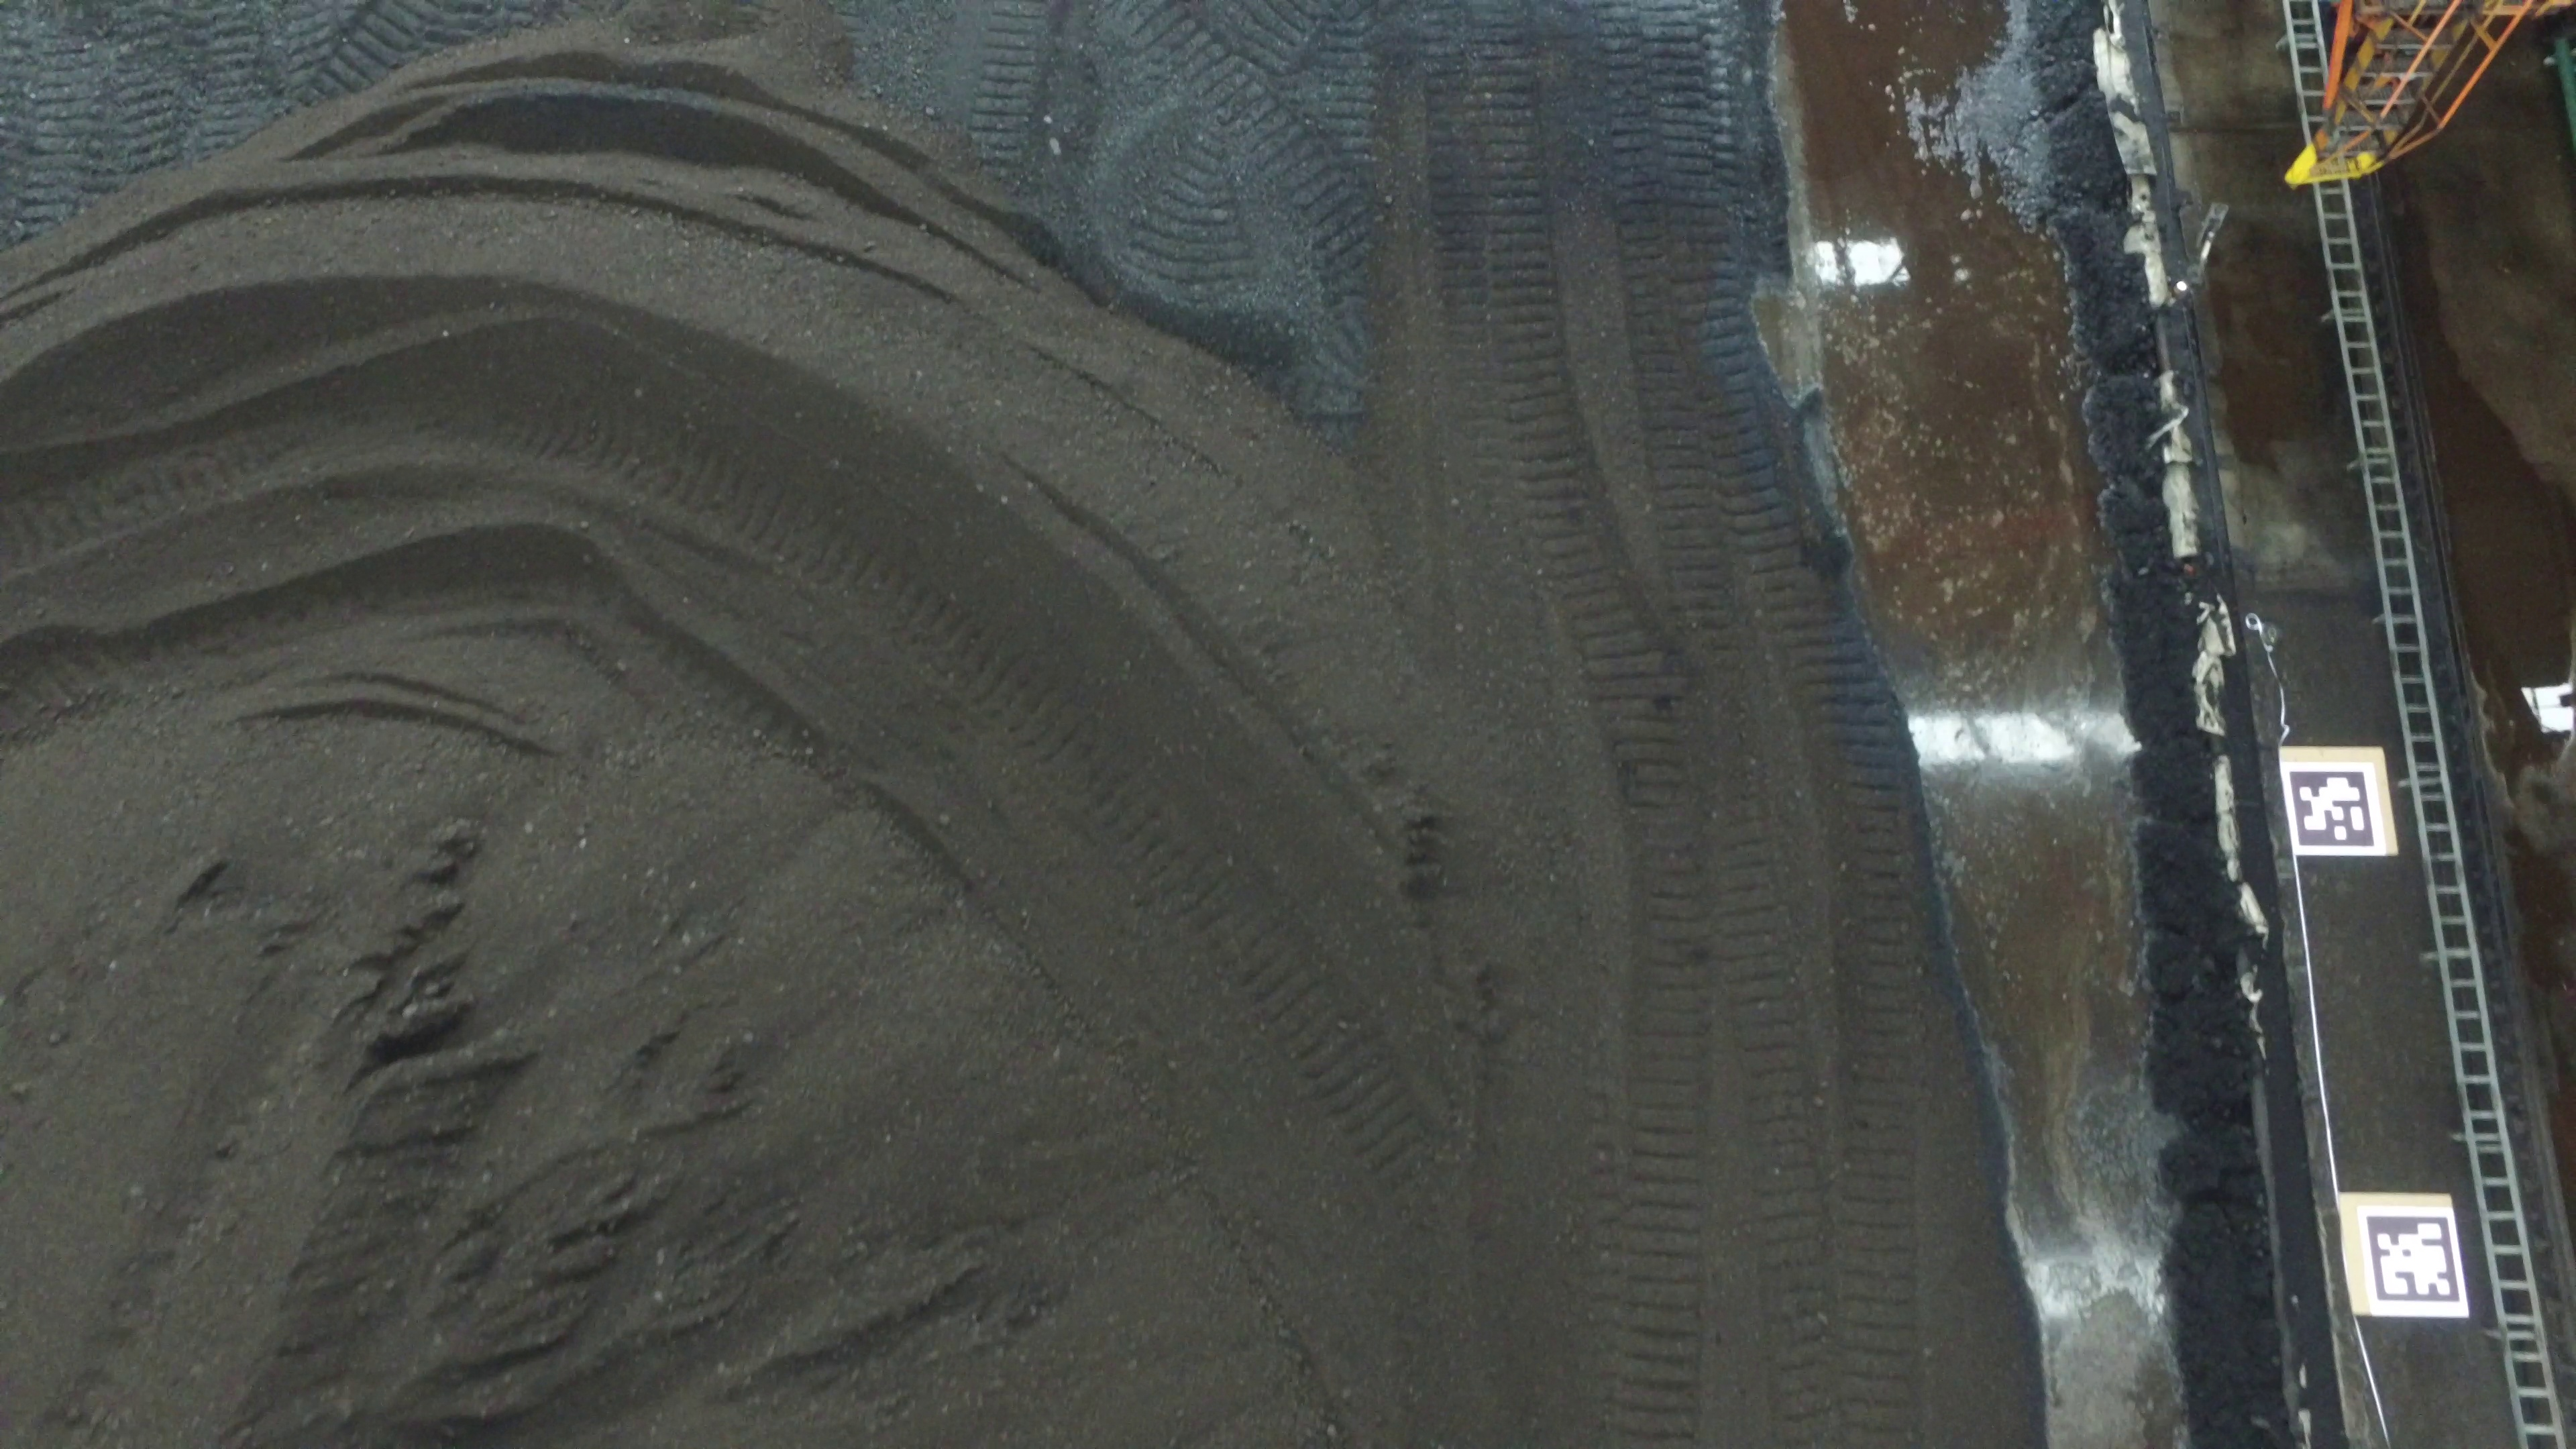
\includegraphics[width=4cm]{2VSLAM_big11.jpg}\hskip1cm}
    \subcaptionbox{Frame12}{\label{fig:2VSLAM_big12}
    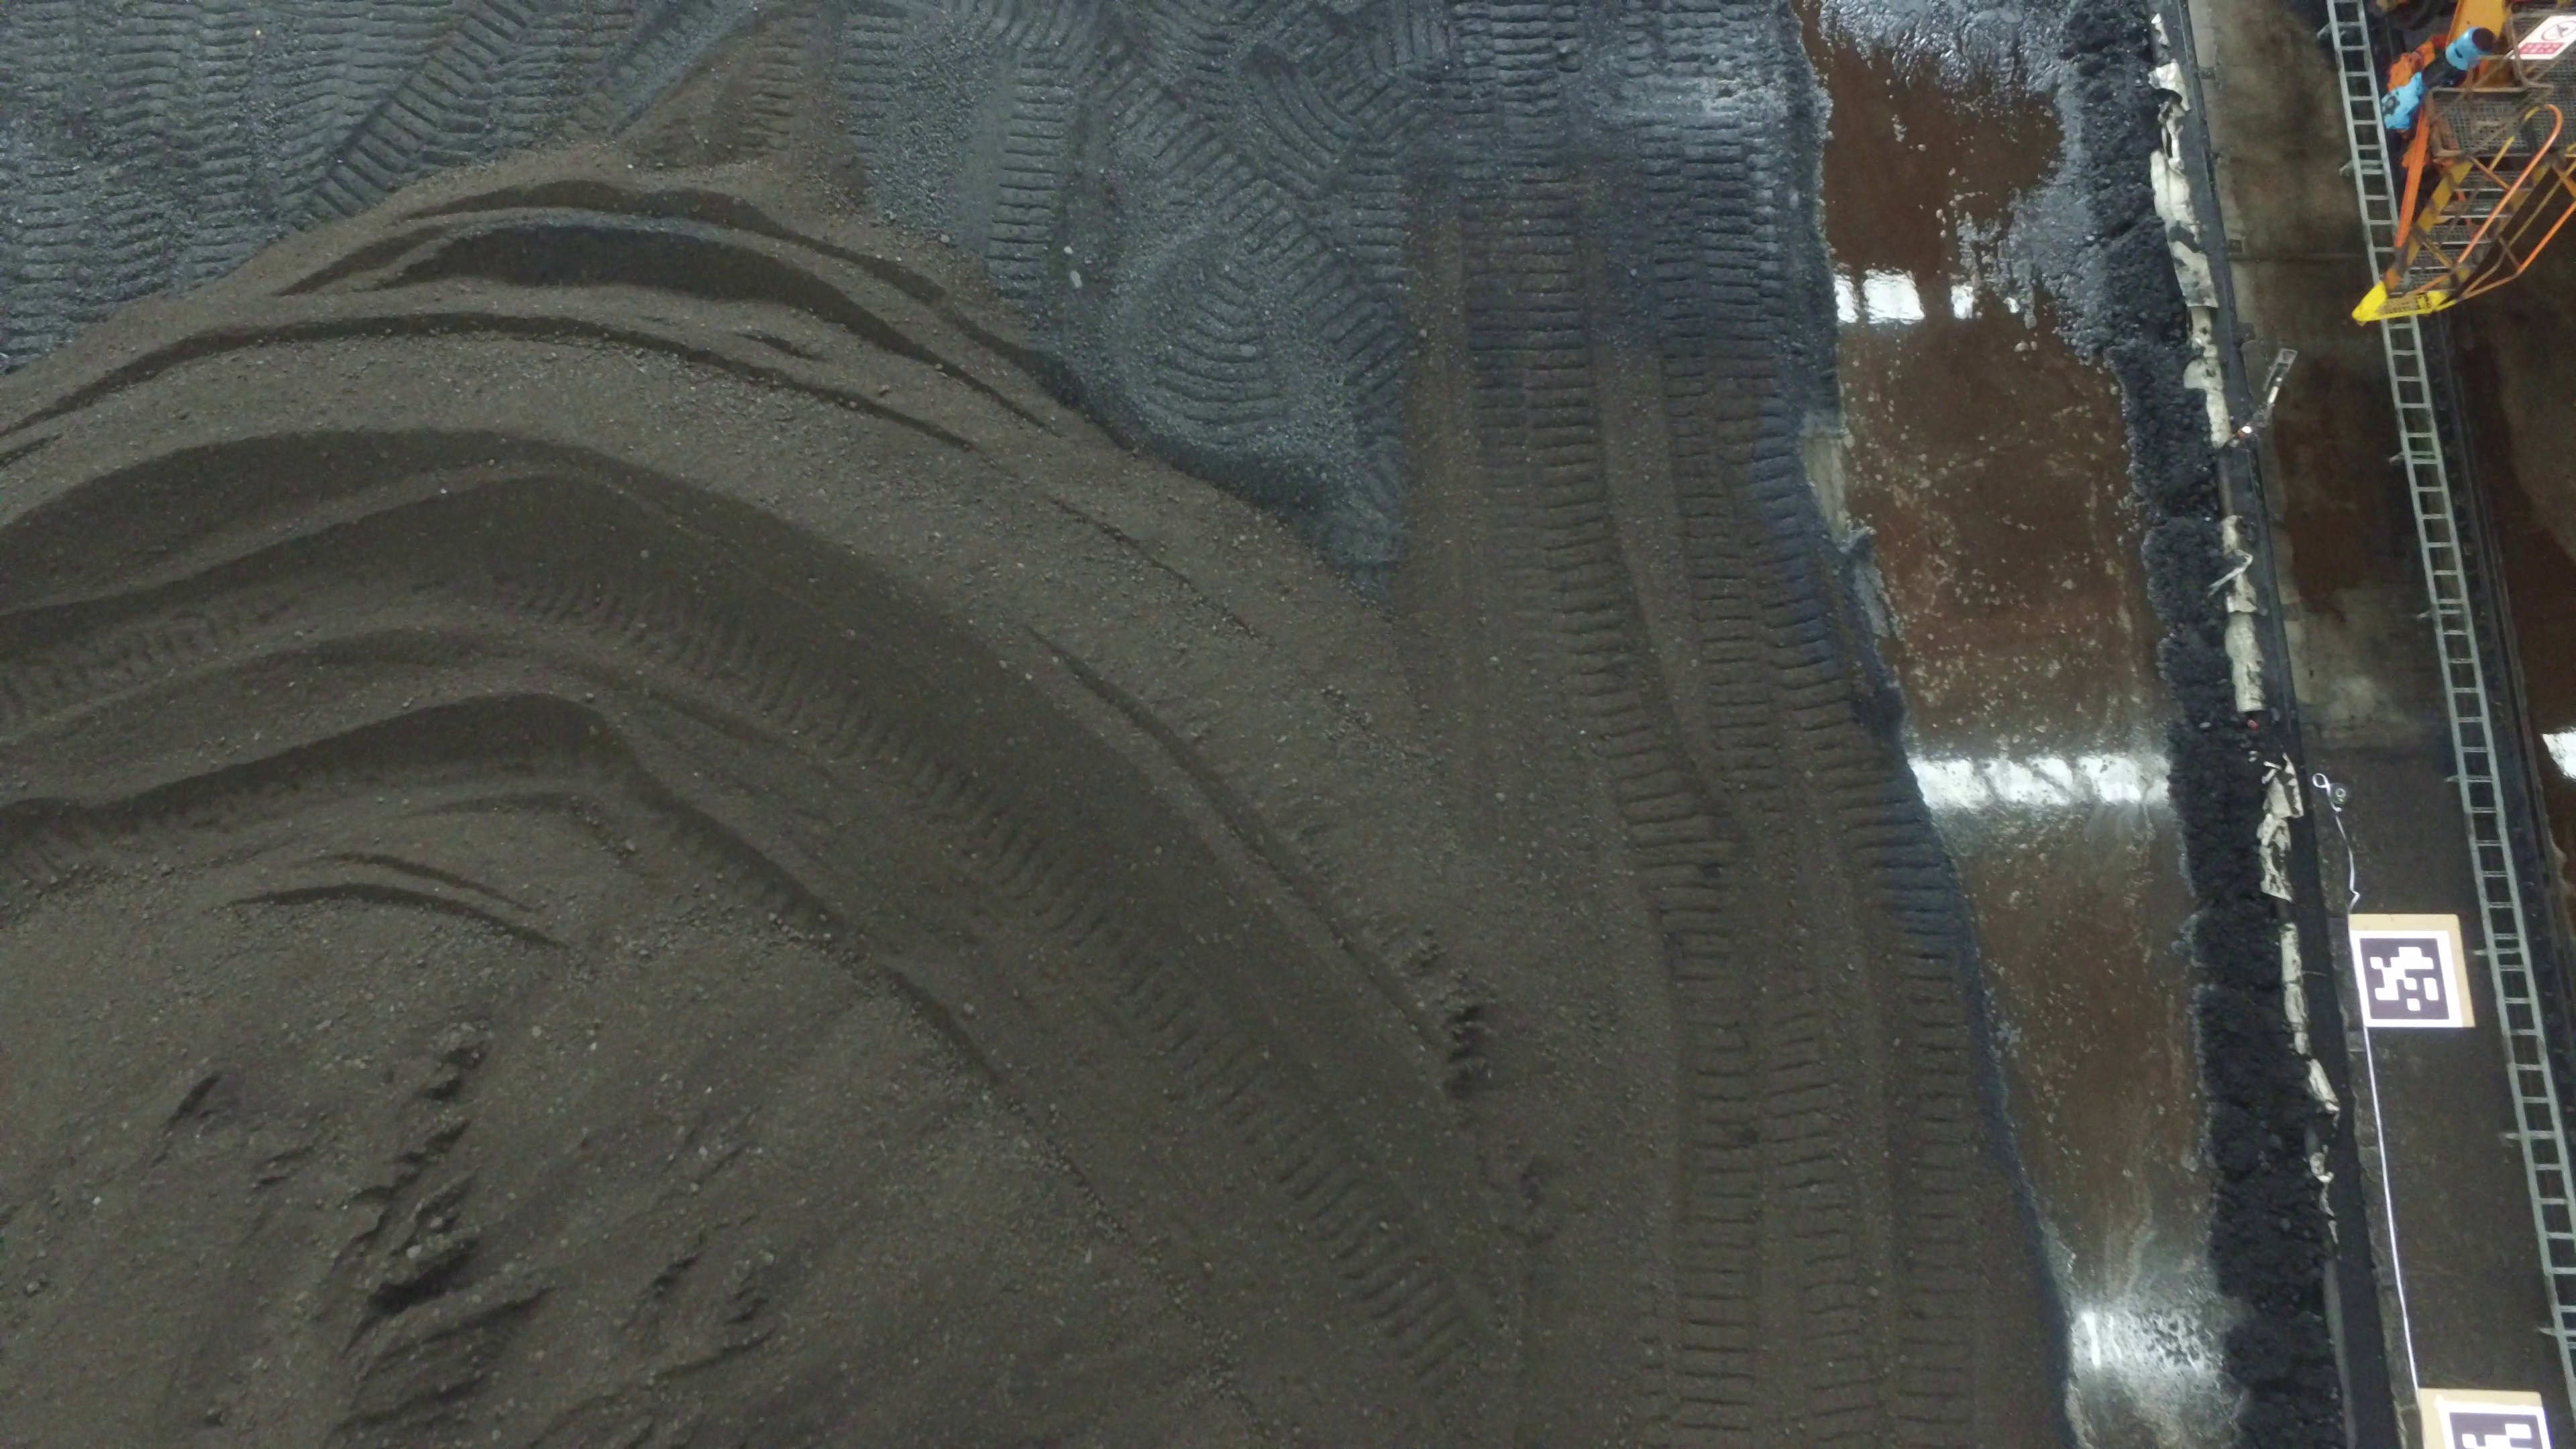
\includegraphics[width=4cm]{2VSLAM_big12.jpg}}

  \caption{无人机采集堆体图像序列}\label{fig:2VSLAM_big}
\end{figure}





\section{本章小结}
\label{sec:2.5}
本章阐述了二维码的检测和识别原理,通过线条和角点的检测,判断区域中二维码的坐标位置以及每一个二维码对应的ID值,推导了通过二维码解算相机位姿的流程。

然后重点研究二维码对视觉SLAM带来的优化作用以及SLAM地图的描述情况,包括关键点,关键帧以及二维码的属性等。说明引入二维码对视觉SLAM各个环节的影响,包括地图初始化、跟踪情况、关键帧的插入筛选、地图优化、回环检测和重定位等。解决了针对堆体场景下,单目视觉SLAM在无人机自主定位工作中,无法确定尺度和不能确定坐标系的问题。

最后本文针对具体堆体场景,进行软件设计,提出了一种为无人机在封闭环境中依靠纯视觉进行自主定位的方案,包括地图管理,图像处理,无人机位姿信息传递等模块,模块之间相互协作,为无人机提供准确的位姿数据,供其后续进行循迹飞行。

在无人机飞行的过程中,会携带图像采集装置,不断采集堆体的图像信息,为后续的堆体三维重建以及体积测量提供支持。 

% \chapter{基于三维重建方法改进}
\label{cha:chap3}
\section{引言}
\label{sec:3.1}
在计算机视觉中,三维重建是指基于对环境或者物体的一系列不同视角的照片,通过特定流程的处理,获得环境或者物体的三维模型,其模型
表达方法众多,常见形式包括点云格式,网格格式,深度地图模式等。三维重建的整个操作流程简易,只需要将采集到的2D图像,或者截取视
频中的图像作为输入,传递给三维重建系统即可,通过一系列的处理即可得到所拍摄场景的3维点云模型,每一个点具备三维位置信息和RGB颜
色信息。三维重建的应用广泛,在自动驾驶,VR,AR等众多领域都有涉及,在未来也会进一步的和计算机视觉中的各种识别方法相互结合,更
好的服务于现代科学。

基于视觉的三维重建的整个流程已经相对比较成熟,在一般情况下,也能得到一个较为满意的结果,但是传统三维重建方法还是存在很多的问
题,三维重建大多数都应用于离线环境,一旦输入数据量较大时,流程本身会十分耗时,且对处理设备的要求也会提升;此外三维重建对场景
的要求也比较高,在光照条件不良,或者场景重复度较高的环境中,三维重建最终输出的点云会存在无法闭合,噪音点对以及场景歧义等现象,
这些都限制了三维重建的应用范围。

基于以上问题,本章将提出一种结合SLAM结果的优化三维重建方法,以解决三维重建耗时和精度不高的问题。三维重建的输入为无序的图像序
列,因此在匹配和解算位姿时都会耗费较大的算力和内存,并且匹配结果因为确实时序信息无法保证匹配的准确性,从而导致后续的位姿解算
也会发生错误。但在SLAM系统中,由于考虑到图像的时序信息,在匹配时不需要进行完全匹配,可以从相邻帧或者回环中检测出匹配对从而节
省算力,此外更加精确的匹配关系能得到更加准确的位姿信息,以为后续三维重建中的稀疏建模和稠密建模获取更高的精度和鲁棒性。
\section{三维重建的一般步骤}
\label{sec:3.2}
三维重建是指从三维图像中复原三维场景或者物体的过程,整个流程的输入为无序的图片即可,输出可以得到三维重建后的稀疏点云和稠密
点,大致流程如图~\ref{fig:3Dconstr_pipiline_sfm}所示。
\begin{figure}[H] % use float package if you want it here
    \centering
    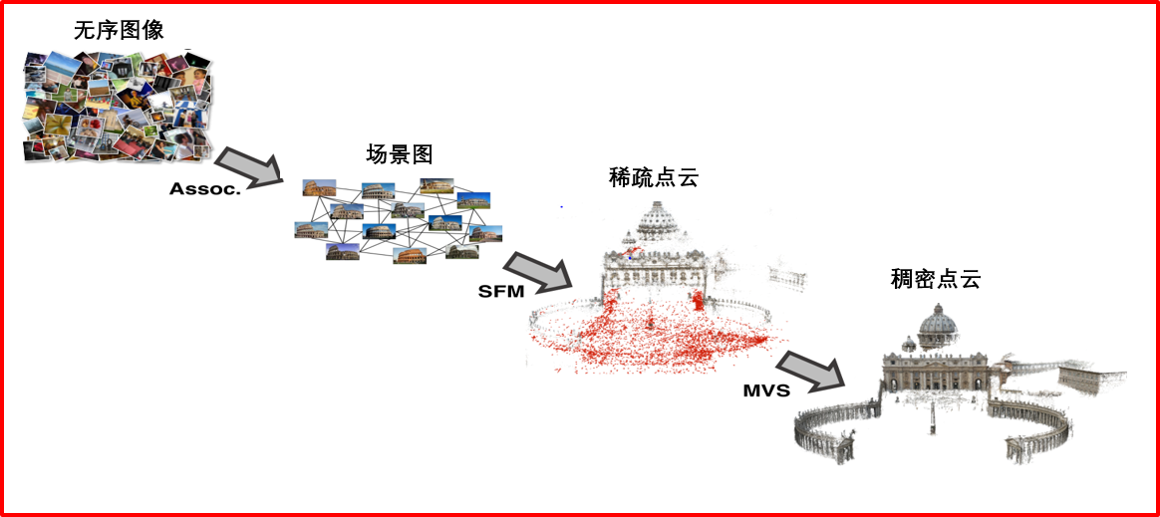
\includegraphics[width=12cm]{3Dconstr_pipiline_sfm.png}
    \caption{三维重建流程图}
    \label{fig:3Dconstr_pipiline_sfm}
    \end{figure}
\subsection{一般方法概述}
\label{sec:3.2.1}
对于以上流程进一步进行细化,整个三维重建的过程可以划分为以下几个主要的步骤:

1.  2D图像采集:多角度拍摄或者从视频中提取到一组图像序列,将图像序列作为整个系统的输入;

2.  特征点提取和匹配:根据拍摄到的图像,提取每张图像之间的特征点,并进行特征点的匹配;

3.  稀疏点云:根据匹配结果估计特征点的深度,提取出稀疏点云,并估计相机的位姿和参数;

4.  稠密点云:根据优化后的相机参数和匹配结果,获得稠密点云;

5.  纹理映射:根据以上点重建物体表面,进行纹理映射。

三维重建的一般步骤可以简化为如图~\ref{fig:3Dconstr_pipiline}所示。
\begin{figure}[H] % use float package if you want it here
    \centering
    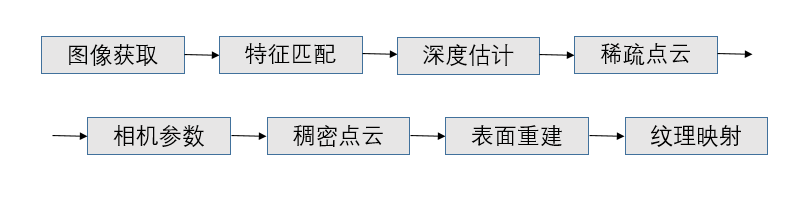
\includegraphics[width=12cm]{3Dconstr_pipiline.png}
    \caption{三维重建一般步骤流程图}
    \label{fig:3Dconstr_pipiline}
    \end{figure}

三维重建主要分为多个步骤,目前很多开源的系统都可以完成其中的部分环节,对于完整的三维重建流程还需要多个系统相互连接实现,
表~\ref{tab:3D_compare}是当前三维重建系统的简要对比。本文在考虑到各个系统流程的完整性和合理性,以及在实际测试过系统之
间的效果差异后,选择Colmap作为作为三维重建的工具。
\begin{table}[h]
    \centering
    \caption{常见三维重建系统对比表}
    \label{tab:3D_compare}
    \begin{tabular}{C{3.6cm}C{2.4cm}C{2.4cm}C{2.4cm}C{2.4cm}}
    \toprule
    \textbf{系统名称} & \textbf{稀疏点云} &\textbf{稠密点云} &  \textbf{重建表面} &\textbf{纹理映射}  \\
    \midrule
    Bundler       &\cellcolor{green}是&\cellcolor{gray}否&\cellcolor{gray}否&\cellcolor{gray}否\\
    CMVS          &\cellcolor{gray}否&\cellcolor{green}是&\cellcolor{gray}否&\cellcolor{gray}否\\
    Colmap        &\cellcolor{green}是&\cellcolor{green}是&\cellcolor{green}是&\cellcolor{gray}否\\
    Meshlab       &\cellcolor{gray}否&\cellcolor{gray}否&\cellcolor{green}是&\cellcolor{green}是\\
    MVE           &\cellcolor{green}是&\cellcolor{green}是&\cellcolor{green}是&\cellcolor{gray}否\\
    MVS-texturing &\cellcolor{green}是&\cellcolor{green}是&\cellcolor{green}是&\cellcolor{gray}否\\
    openMVG       &\cellcolor{green}是&\cellcolor{green}是&否\cellcolor{gray}&\cellcolor{gray}否\\
    openMVS       &\cellcolor{gray}否&\cellcolor{gray}否&\cellcolor{green}是&\cellcolor{green}是\\
    Theia         &\cellcolor{green}是&\cellcolor{gray}否&\cellcolor{gray}否&\cellcolor{gray}否\\
    VisualFSM     &\cellcolor{green}是&\cellcolor{green}是&\cellcolor{gray}否&\cellcolor{gray}否\\
    \bottomrule
    \end{tabular}
  \end{table}
\subsection{三维重建详细过程解析}
\label{sec:3.2.2}
\subsubsection{图像获取} 
\label{sec:3.2.2.1}
目前常规的三维重建仅需要输入无序图片,在构图的过程中,可以极大地降低操作的复杂度,并且对于相机的内参和外参也无需提前提供给整
个三维重建的系统,在特征点匹配的过程中,这些参数都可以通过计算得到。对于输入的图像,可以通过随着时间流单帧拍摄的方式获取或者
通过截取视频流的方式得到,且图像之间不能仅有纯旋转,这样无法估计深度。在获取图像的过程中,需要注意保证每连续两帧图像之间尽可
能保证30$\%$的重叠区域,相邻两帧之间的旋转角度为30度到45度之间,且物体中的每一个点至少能被三帧图像观测到。
\subsubsection{特征点的检测和匹配} 
\label{sec:3.2.2.2}
特征是图像信息的另外一种数字表现形式,良好的特征应该是不受光线,噪音,几何变形影响的。特征提取的目的是为了后续能够尽可能准确、稳
定地估计出相机的运动,特征点能够具备可重复性,高效率,可区别性以及本地性的特点,经过几十年的发展,在图像处理领域已经提出了多种特
征提取的方法。

\textbf{Harris角点:}当从不同的方向去移动一个视觉窗口,假设该区域内的灰度发生了很大的的变化,则认定存在角点。对于图像I(x,y),
当在点(x,y)处平移(Δx,Δy)后的对应窗口的像素点灰度变化描述为:
\begin{equation}
  c(x, y ; \Delta x, \Delta y)=\sum_{(u, v) \in W(x, y)} (I(u, v)-I(u+\Delta x, v+\Delta y))^{2}
  \label{equ:Harris}
\end{equation}
结合泰勒分解公式,上式可以化简为:
\begin{equation}
  c(x, y ; \Delta x, \Delta y) \approx \sum_{w}\left(I_{x}(u, v) \Delta x+I_{y}(u, v) \Delta y\right)^{2}=[\Delta x, \Delta y] M(x, y)\left[\begin{array}{c}{\Delta x} \\ {\Delta y}\end{array}\right]
\end{equation}
其中
\begin{equation}
  \begin{split}
   & M(x, y)=\sum_{w}\left[\begin{array}{cc}{I_{x}(x, y)^{2}} & {I_{x}(x, y) I_{y}(x, y)} \\ {I_{x}(x, y) I_{y}(x, y)} & {I_{y}(x, y)^{2}}\end{array}\right]\\
   & =\left[\begin{array}{cc}{\sum_{w} I_{x}(x, y)^{2}} & {\sum_{w} I_{x}(x, y) I_{y}(x, y)} \\ {\sum_{w} I_{x}(x, y) I_{y}(x, y)} & {\sum_{w} I_{y}(x, y)^{2}}\end{array}\right] \\
   & =\left[\begin{array}{cc}{A} & {C} \\ {C} & {B}\end{array}\right] 
  \end{split}
  \end{equation}
公式~\ref{equ:Harris}即可转化为
\begin{equation}
  c(x, y ; \Delta x, \Delta y) \approx A \Delta x^{2}+2 C \Delta x \Delta y+B \Delta y^{2}
\end{equation}
又提出角度响应值R来判断该点是否为角点:
\begin{equation}
  R=\operatorname{det} \boldsymbol{M}-\alpha(\operatorname{trace} \boldsymbol{M})^{2}
\end{equation}
通过以上公式可以看出,Harris角点具备以下特点:\\
1. 对亮度和对比度的变化不敏感:因为微分运算对图像密度的变化不敏感,即亮度或者对比度的变化对Harris的检出影响较小;\\
2. 具有旋转不变性:Harris角点检测算子的本质可以表示为一个椭圆,但椭圆旋转时,并不会影响R值的大小;\\
3. 不具有尺度不变性。

\textbf{FAST特征点:}对图像中的中的一个像素p,假设其亮度值为$I_p$,阈值为t,如图所示,取以其为中心,半径为是三个像素的圆,
圆上共有16个像素点,假设这16个点中有连续N个点都比$I_p+t$大或者比$I_p-t$小,则认定其为Fast角点,为了加快检测过程,会直接检
测第1,5,9,13这4个点,如果有三个满足要求,也会认为是角点。
\begin{figure}[H] % use float package if you want it here
  \centering
  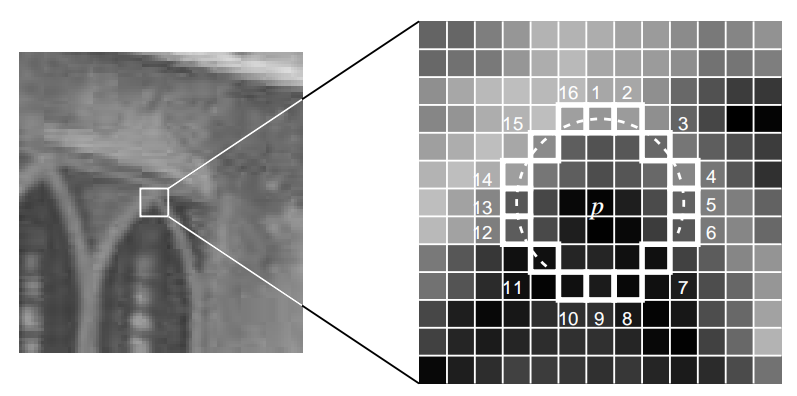
\includegraphics[height=6cm]{2VSLAM_Fast.png}
  \caption{FAST特征点}
  \label{fig:2VSLAM_Fast}
\end{figure}
\textbf{ORB特征点:}结合了FAST特征点的检测和BRIEF描述子,其中RIEF特征描述符的计算过程:首先平滑图像,在某个像素点的周围选
择一个领域,根据特定的点对选择方法挑选出$n_d$个点对,比较每个点对之间亮度值的大小,即可得到一个长度为$n_d$的二进制串。
由于FAST特征点不具有方向,ORB在此基础上进行了改良,即利用灰度质心法求解出灰度额质心之间的偏移方向,首先定义特征点p的邻域像素的矩:
\begin{equation}
  m_{p q}=\sum_{x, y} x^{p} y^{q} I(x, y)
\end{equation}
图像的质心为:
\begin{equation}
  C=\left(\frac{m_{10}}{m_{00}}, \frac{m_{01}}{m_{00}}\right)
\end{equation}
那么偏移方向可以定义为FAST的特征点方向:
\begin{equation}
  \theta=\arctan \left(m_{01}, m_{10}\right)
\end{equation}
通过以上内容说明了SLAM框架中常用的特征点提取方式,接下来将以此为基础说明特征点的匹配过程:即在已知参考帧和当前参考帧的特征点
信息时,求解这两帧中相同的特征点。计算两帧中的汉明距离是常用的特征匹配方法,即计算两个等长描述符对应位置上不同数字的个数,数
值越小,越相似。如图~\ref{fig:2VSLAM_ORB_match}所示为通过提取ORB特征进行匹配的结果。
\begin{figure}[H] % use float package if you want it here
  \centering
  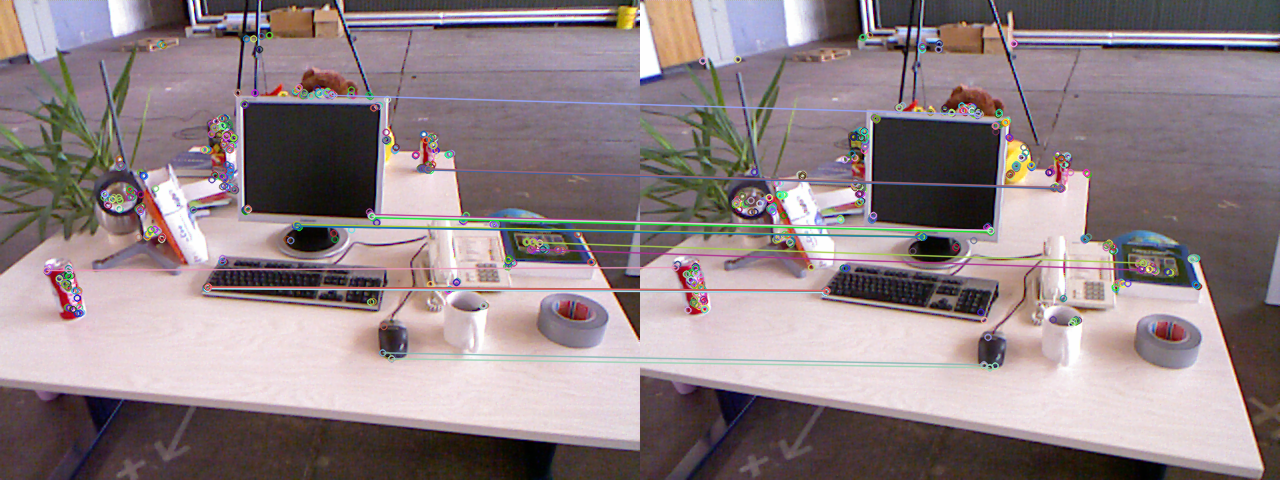
\includegraphics[height=6cm]{2VSLAM_ORB_match.png}
  \caption{ORB特征匹配结果}
  \label{fig:2VSLAM_ORB_match}
\end{figure}

目前,在三维重建领域中图像的特征匹配就是以特征点为基础而进行的,所以,如何定义和找出一幅图像中的特征点就非常重要。常见的
特定点检测和匹配主要包括SUFT,SIFT,ORB,Harris角点等,各方法的简要特点如表所示。
\begin{table}[h]
    \centering
    \caption{常见特征检测方法对比表}
    \label{tab:Feature}
    \begin{tabular}{C{4.6cm}L{8.4cm}}
    \toprule
    \textbf{方法名称} & \textbf{特点}  \\
    \midrule
    SUFT&解决特征检测中的尺度不变性问题,具备较高的计算效率\\
    SIFT&以SUFT为基础,基于浮点内核计算特征点,有着更加精确的空间位置和尺度\\
    ORB&满足实时性的速度,但是不具备旋转,尺度不变性且噪声敏感\\
    Harris角点&能够较好的检测角点,进行精确的定位\\
    \bottomrule
    \end{tabular}
  \end{table}

对于本文中的三维重建,选择SIFT作为特征点的检测和匹配方法,针对其计算耗时的问题,本文选择CUDA进行硬件加速,另外还考虑到三维
重建本身是一个离线处理的过程,对算法的实时性没有过高要求。SIFT和其他方法相比较,有以下优点:\\
1. SIFT特征是图像的局部特征,其对旋转、尺度缩放、亮度变化保持不变性,对视角变化、仿射变换、噪声也保持一定程度的稳定性;\\
2. 独特性好,信息量丰富,适用于在海量特征数据库中进行快速、准确的匹配;\\
3. 多量性,即使少数的几个物体也可以产生大量的SIFT特征向量。\\
如图~\ref{fig:3Dconstrmatchresult}所示,分别对两帧图形提取SIFT特征,随后根据特征点进行匹配。
\begin{figure}[H]
    \centering
      \subcaptionbox{第1帧图像提取SIFT特征}{\label{fig::3Dconstr_a}
      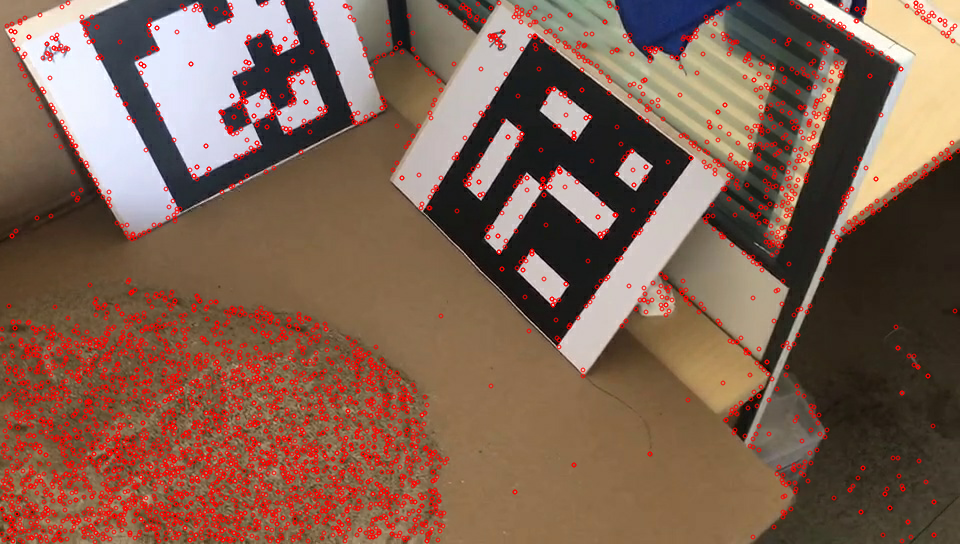
\includegraphics[width=6cm]{3Dconstr_a.png}\hskip2cm}
      \subcaptionbox{第2帧图像提取SIFT特征}{\label{fig:3Dconstr_b}
      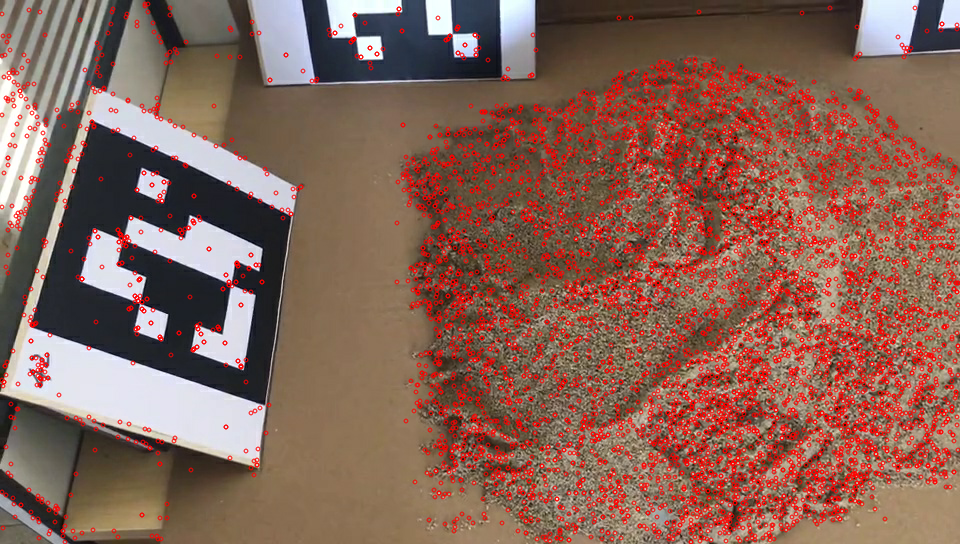
\includegraphics[width=6cm]{3Dconstr_b.png}}
    \vskip0.5cm
      \subcaptionbox{根据特征点进行匹配\label{fig:chap03:3Dconstr_match}}{
      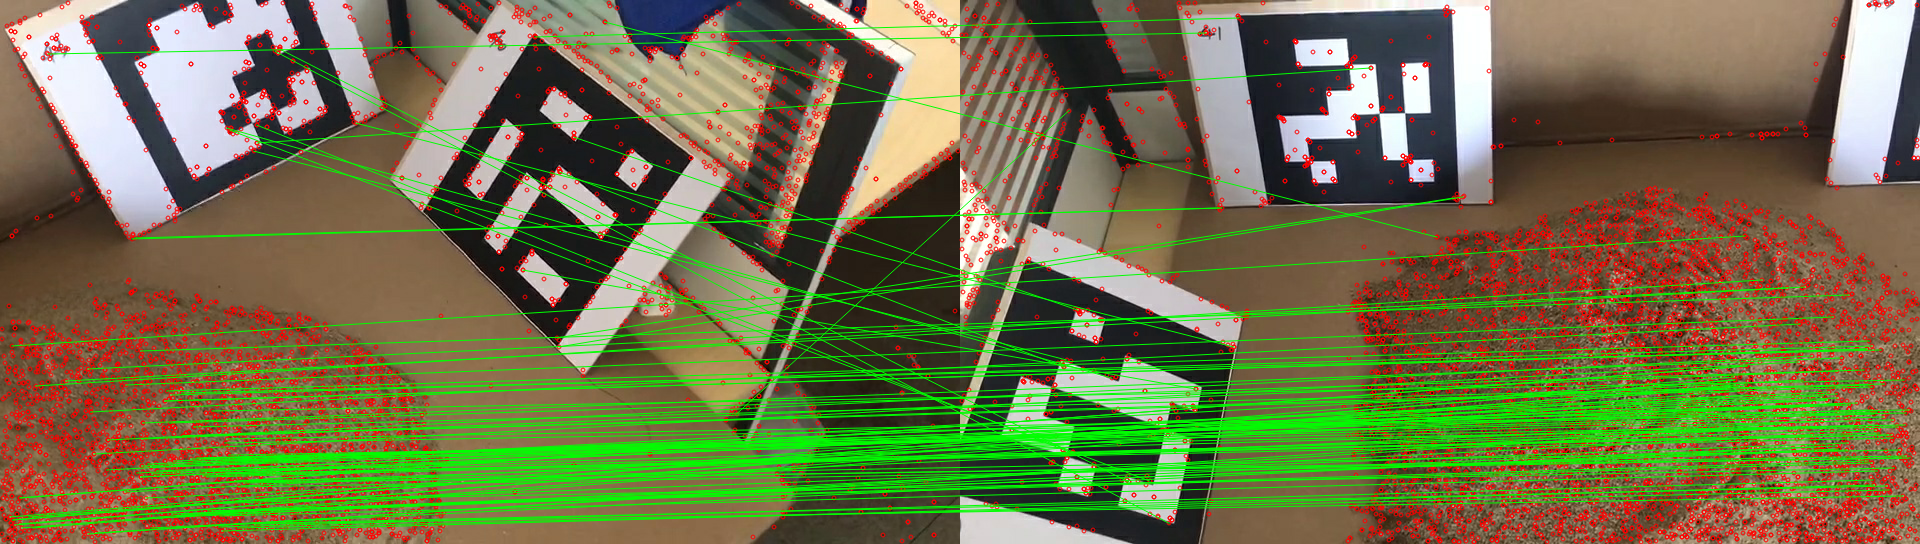
\includegraphics[width=12cm]{3Dconstr_match.png}\hskip2cm}
    \caption{特征提取与匹配结果示意图}\label{fig:3Dconstrmatchresult}
  \end{figure}
在获取到每张图像上的特征点后,需要对图像之间建立匹配关系,常用的方式可以采用计算欧式距离的办法:1)完全匹配,对所有的特征
点都进行穷举,计算其对应距离。2)邻近搜索,建立KD树,缩小搜索范围,能提高效率,但也有可能不是最优,所以邻域取值是关键,越大越准
确,越大计算量越大。由图~\ref{fig:chap03:3Dconstr_match}~所示,两帧之间大多数特征点都可以正确匹配,但依然存在存在部分匹配
是错误的,在本文中,选择了RANSAC(随机抽样一致性)的方式来剔除错误的匹配对,以更加准确的估计相机位姿,RANSAC是指可以从一组
包括局外点(错误匹配)的观测数据中,通过迭代的方式估计数学模式中的参数,通过RANSAC处理后的匹配结果如
图~\ref{fig:3Dconstr_matchAfterRansac}所示,误检的匹配已经被明显的降低。
\begin{figure}[H] % use float package if you want it here
  \centering
  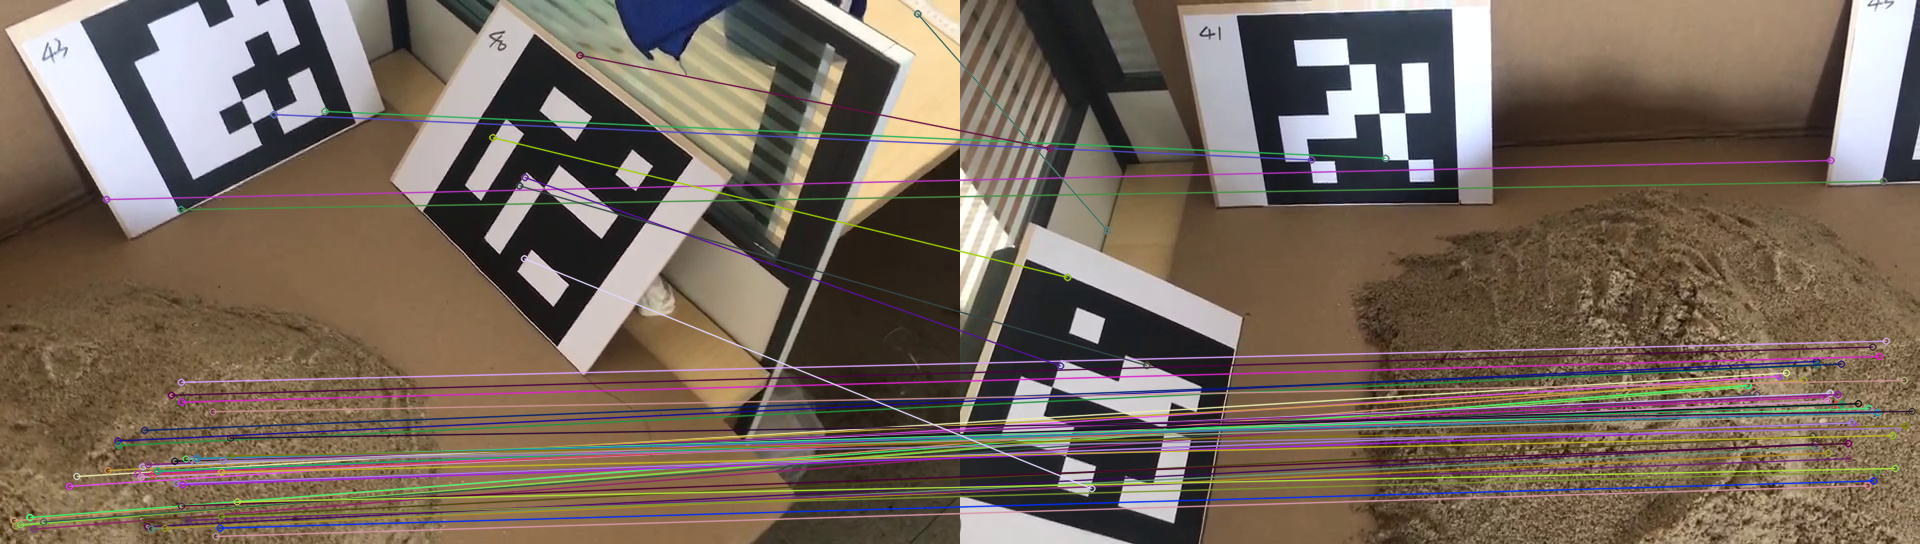
\includegraphics[width=12cm]{3Dconstr_matchAfterRansac.png}
  \caption{RANSAC之后的点云匹配}
  \label{fig:3Dconstr_matchAfterRansac}
  \end{figure}
\subsubsection{SfM} 
\label{sec:3.2.2.3}
在~\ref{sec:3.2.2.2}小节中,可以获得初始的匹配关系,但是这种匹配关系不完全可靠,需要添加几何约束进行检测,该集合约束完全依
赖于场景中的客观事实。可以通过基本矩阵F将匹配好的两帧图像之间的像素坐标(x,y),(x',y')进行关联,假设一个符合条件的匹配对像素坐标需要满足以
下公式:
\begin{equation}
\begin{bmatrix}x'&y'&z'\end{bmatrix}\mathrm F\begin{bmatrix}\mathrm x\\\mathrm y\\\mathrm z\end{bmatrix}=0
\end{equation}

找到相机基线最大的像对,根据该像对,通过RANSC八点法计算本征矩阵,再通过对本征矩阵SVD分解得到第二个图像的R、T,在这一步需要进行畸变校正,
然后根据R、T和矫正后的像点坐标三角计算出三维点。

当所有的两两匹配图像对被确定以后,可以开始计算相机的位姿(3*3的旋转矩阵R,1*3的平移向量t),摄像机的内参(焦距f,畸变参数
k1,k2)。几何场景提供轨迹中的每个3D点$X_j$,通过投影方程,将3D点投影到摄像机的2D成像平面上,投影误差的定义为投影点和图像上
真实点之间的欧式距离,如图~\ref{fig:3Dconstr_reprojection-error}所示。
\begin{figure}[H] % use float package if you want it here
  \centering
  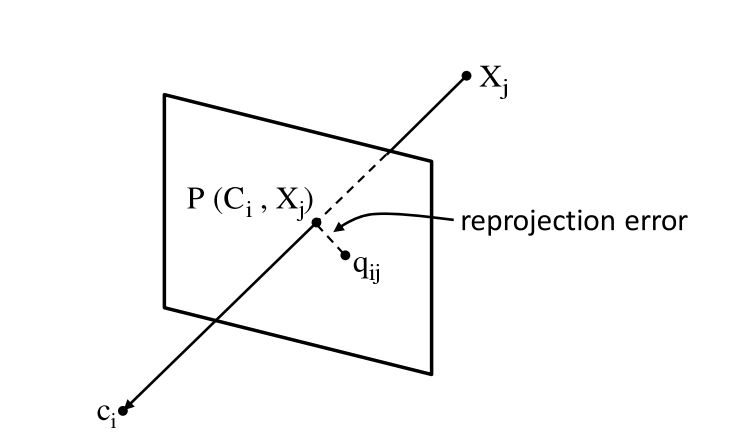
\includegraphics[width=8cm]{3Dconstr_reprojection-error.png}
  \caption{误差投影示意图}
  \label{fig:3Dconstr_reprojection-error}
\end{figure}
对于n个视角和m个轨迹,投影误差的目标优化方程为:
\begin{equation}
  \mathfrak g(C,X)=\sum_{i=1}^n\sum_{j=1}^m\omega_{ij}\left|\left|q_{ij}-P(C_i,X_j)\right|\right|^2
\end{equation}
其中$\left|\left|q_{ij}-P(C_i,X_j)\right|\right|^2$就是摄像机i中的轨迹j的投影误差累积和,SFM算法的目标就是找到合适的相机
和场景参数去优化这个目标函数,g是采用一个非线性最小二乘的优化方法求解,常用BA(光束平差法)来优化上述过程。
最后,不断添加新的摄像机和3D点进行BA。这个过程直到剩下的摄像机观察到的点不超过20为止,说明剩下的摄像机没有足够的点可以添加,
BA结束。得到相机估计参数和场景几何信息,即稀疏的3D点云。
\subsubsection{MVS} 
\label{sec:3.2.2.4}
SfM是指从运动中恢复结构的过程,而MVS则是多视角立体视觉生成统,SfM生成的是稀疏点云,恢复相机之间的几何关系,MVS生成的是稠密
点云,由SfM获得的一些相机参数和相机之间的几何关系,来进行MVS。在SfM中,重建的点都是由特征匹配的点,这些点集本身就就不稠密,
因此无法获取到稠密的点云,而在三维重建的过程就需要通过MVS的方式获取稠密的点集,MVS利用图像中的像素点来实现点云的重建,将图
像中的每一个像素点估计其三维坐标,构成稠密点云。

在稠密点云的估计过程中,无法将每一个像素点按照特征点的方式计算其描述子,因此提出了极线搜索和快匹配技术来匹配图像中的某一像素
点在其他图像中的对应的点,在找到每一个像素点在其他图像中出现的位置之后,就可以利用三角测量的发放确定其深度,但是因为用一个像
素点会出现在多个图像中,所以就期望通过多次三角化让该点的深度值收敛。

对于极线搜索和块匹配技术,如图~\ref{fig:3Dconstr_jixiansousuo}所示。
\begin{figure}[H] % use float package if you want it here
  \centering
  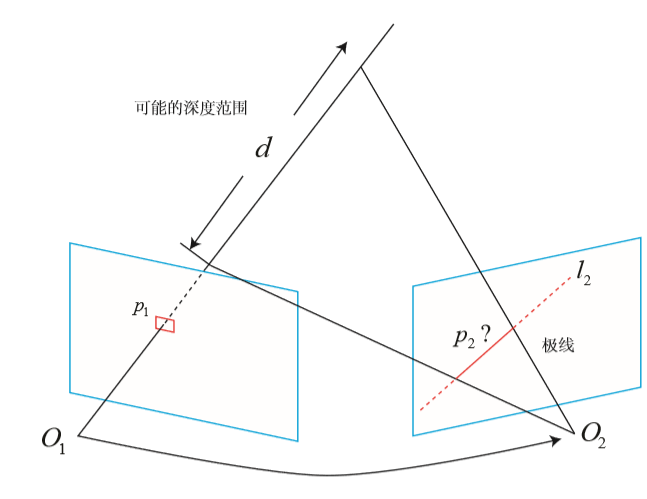
\includegraphics[width=8cm]{3Dconstr_jixiansousuo.png}
  \caption{极线搜索示意图}
  \label{fig:3Dconstr_jixiansousuo}
\end{figure}
首先对于极线搜索和块匹配技术,如图所示,左侧的相机观测到了像素点$p_1$,由于该相机为单目相机,没法确定深度,可以先假设该点的
实际位置在0到正无穷的区间中,因此该像素对应的空间点就分布在某条线段上,对于右侧相机,上述线段可以在成像平面上生成一段投影,在已知
两帧图像之间的相对位姿时,是可以确定该极线的位置的,接下来就需要在极线上寻找与像素点$p_1$所对应的$p_2$点的位置。

因为单个像素没有对应的特征值,无法进行匹配,此外依靠单个特征点的亮度来进行匹配也并不可靠,可以基于图像块在前后变化得到过程
中的灰度不变性特征,在P1周围选育一块w*w得到小块,然后在右侧的极线上选择多个这样的小块来提高区分度。对于计算两个小块之间的
差异,一般可以通过以下方法来计算:\\
1.SAD取两个小块的差的绝对值之和
\begin{equation}
  S{(A,B)}_{SAD}=\sum_{i,j}\left|A(i,j)-B(i,j)\right|
\end{equation}
2.SSD取两个小块比较求平方和
\begin{equation}
S{(A,B)}_{SSD}=\sum_{i,j}(A(i,j)-B{(i,j))}^2
\end{equation}
3.NCC取两个小块计算相似性
\begin{equation}
  S{(A,B)}_{NCC}=\frac{{\displaystyle\sum_{i,j}}A(i,j)B(i,j)}{\sqrt{{\displaystyle\sum_{i,j}}A{(i,j)}^2\underset{i,j}\sum B{(i,j)}^2}}
\end{equation}

在极线上,计算了 A 与每一个 Bi 的相似性yo度量,那么将得到一个沿着极线的数值分布,该分布的形状取决于图像本身信息,在搜索距
离较长的情况下,通常会得到一个非凸函数:该分布存在许多峰值,但是真实值只有一个,接下来需要使用深度滤波器使用概率分布来描述
深度值从而找到对应的$p_2$点。
\subsection{当前三维重建存在的问题}
\label{sec:3.2.3}
根据~\ref{sec:3.2}节的描述,可以发现通过现有的三维重建技术流程可以实现有多张连续图像到三维点云的转化,整个过程操作起来十分
简便,且能够得到一个较好的结果。但是从整体实验速度,三维点云结果的精确性来看,依然还存在很多的问题:\\
1. 三维重建对场景中物体的表面纹理要求较高,对于纹理重复的场景或者贫纹理的场景,三维重建的结果就难以复现出场景的实际的结果,
无法生成地图信息。\\
2. 整个三维重建的过程十分耗时,由于三维重建中的图像时间没有时序信息,关键帧之前的匹配都通过完全枚举的方式进行匹配,对于输入
N张原始图像的系统,时间复杂度高达O($N^2$),由单帧图像到稀疏点云一般耗时为几分钟,由单帧图像到稠密点云耗时耗时更是会高度几
个小时。\\
3. 独三维点云的精度不高,噪音点较大,一方面是由于三维重建往往采取增量式的重建方式,导致最终场景重建的结果无法闭合;另外一方
面也是由于对于某些重复度较高的场景,关联帧之间的匹配由于缺少时序信息,从而导致匹配精度较低,在解算相机位姿时,得到的结果也无
法保证正确,如图~\ref{fig:chap2:3dconstr_stone}所示。
\begin{figure}[htbp]
  \centering
    \subcaptionbox{正面}{\label{fig:chap1:3dconstr_stone1}
    \includegraphics[width=4cm,height=5cm]{3dconstr_stone1.JPG}}
    \subcaptionbox{斜侧面}{\label{fig:chap1:3dconstr_stone2}
    \includegraphics[width=4cm,height=5cm]{3dconstr_stone2.JPG}}
    \subcaptionbox{侧面}{\label{fig:chap1:3dconstr_stone3}
    \includegraphics[width=4cm,height=5cm]{3dconstr_stone3.JPG}}
  \vskip0.5cm
  \subcaptionbox{无法闭合}{\label{fig:chap1:3Dconstr_stone1}
  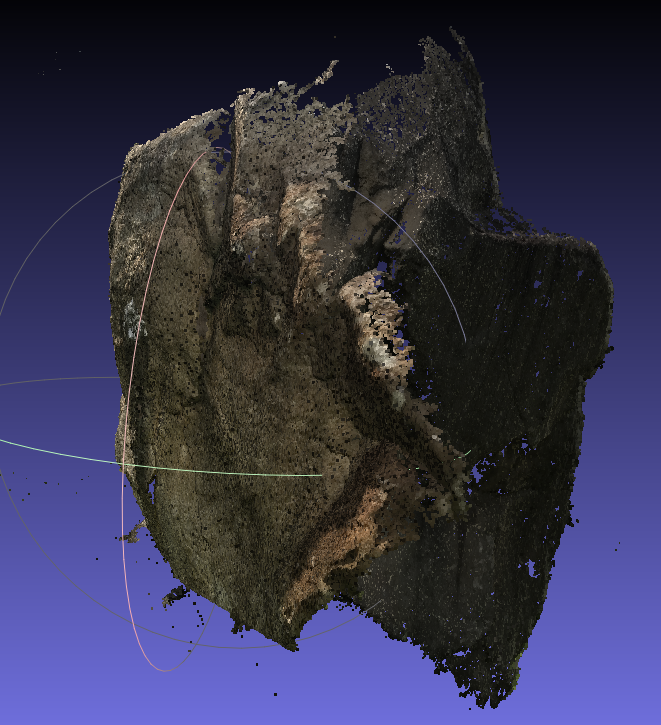
\includegraphics[width=4cm,height=5cm]{3Dconstr_stone1.png}}
  \subcaptionbox{缺失较多}{\label{fig:chap1:3Dconstr_stone2}
  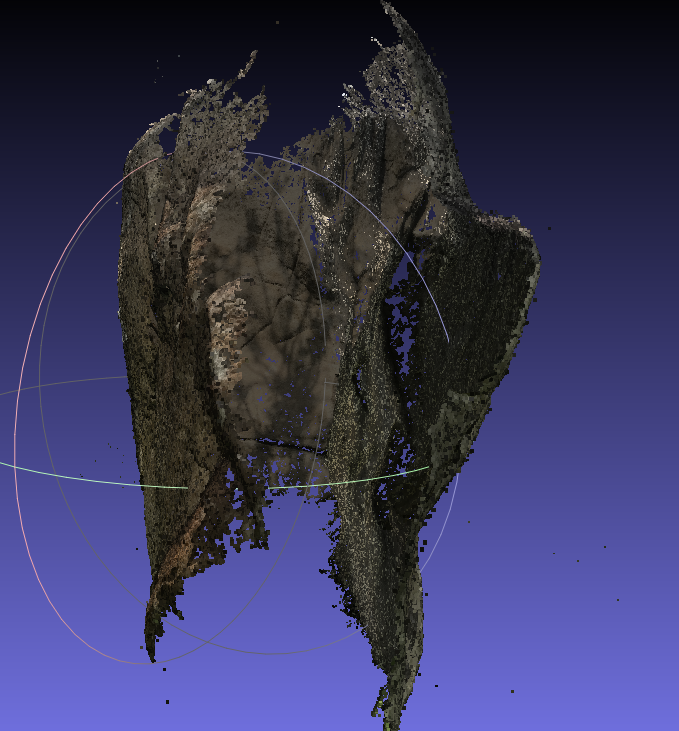
\includegraphics[width=4cm,height=5cm]{3Dconstr_stone2.png}}
  \subcaptionbox{噪音点多}{\label{fig:chap1:3Dconstr_stone3}
  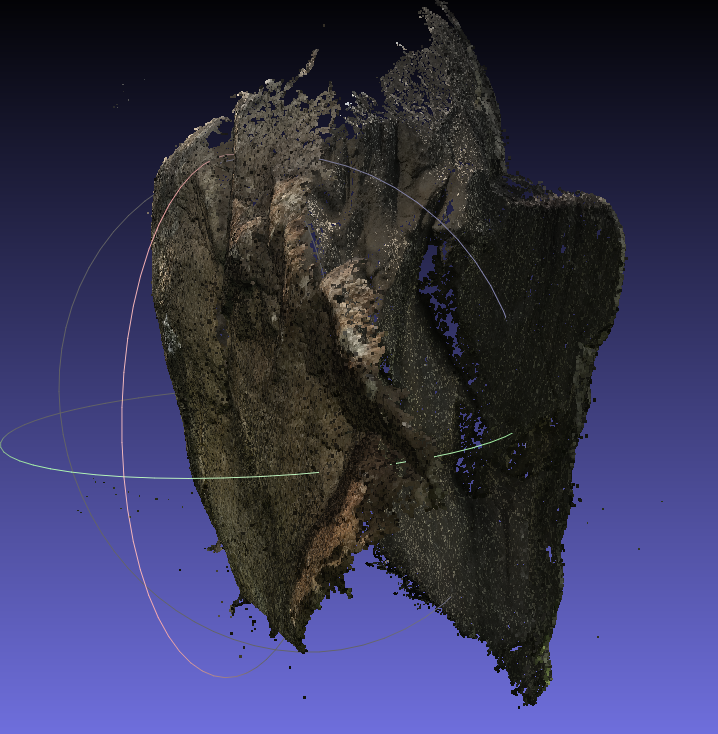
\includegraphics[width=4cm,height=5cm]{3Dconstr_stone3.png}}
  \caption{自然场景三维重建结果示意图}\label{fig:chap2:3dconstr_stone}
\end{figure}
\section{三维重建的优化讨论}
\label{sec:3.3}
% \subsection{解决贫纹理方案}
% \label{sec:3.3.1}
% 对于一些常见的工业工件,多由金属构成,表面光滑无显著纹理信息,如图~\ref{fig:3Dconstr_iron1}所示,在特征提取环节难以提取到特
% 征对,对于后续的匹配和三角化过程都难以进行,且在以光源下,存在很严重的反光问题,对于不同视角下会生成不同的图像信息影响建模。
% 因此现在提出一种在金属器件表面涂上荧光剂的方法来改良贫纹理工件难以三维建模的问题,如图~\ref{fig:3Dconstr_iron2}所示。
% \begin{figure}[H]
%   \centering%
%   \subcaptionbox{金属工件原图\label{fig:3Dconstr_iron1}}{%    
%     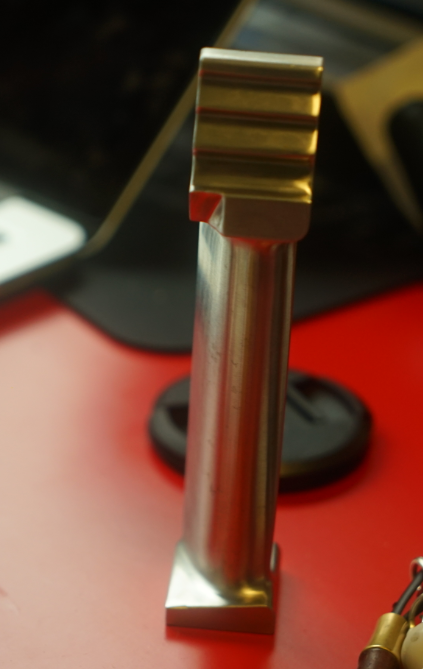
\includegraphics[height=6cm]{3Dconstr_iron1.png}}\hspace{2em}%
%   \subcaptionbox{金属工件添加荧光剂示意图\label{fig:3Dconstr_iron2}}{%    
%     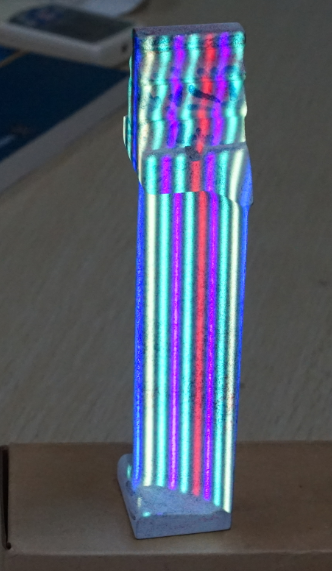
\includegraphics[height=6cm]{3Dconstr_iron2.png}}
%   \caption{金属工件示意图}
%   \label{fig:3Dconstr_iron}
% \end{figure}
% 按照~\ref{sec:3.2}节的流程,可以获得如图~\ref{fig:3Dconstr_iron3}所示的三维点云结果图。
% \begin{figure}[H] % use float package if you want it here
%   \centering
%   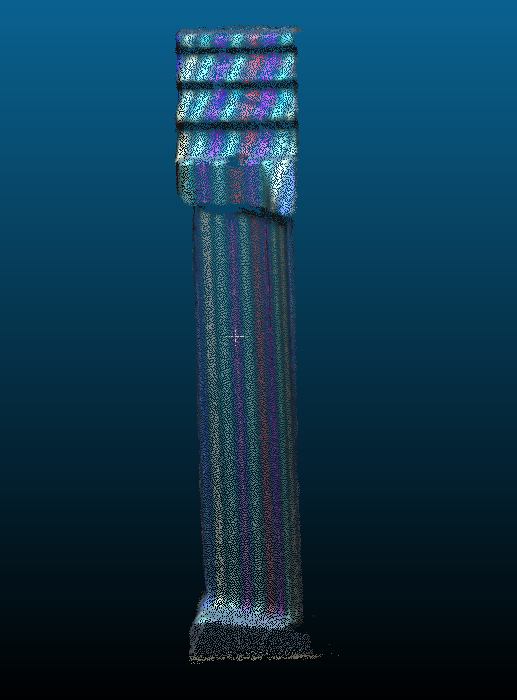
\includegraphics[height=9cm]{3Dconstr_iron3.png}
%   \caption{金属工件三维重建结果示意图}
%   \label{fig:3Dconstr_iron3}
% \end{figure}
\subsection{增加实效性方案}
\label{sec:3.3.2}
在对无序的图像进行三维重建时,会有大量的时间耗费在图像的匹配过程中,在三维重建中常见的图像匹配方法以下几种方法:

1.  完全匹配:当用于三维重建的图像数量较低时,这种匹配模式一般可以较快的完成,并且产生一个比较好的匹配结果,在这种模式里,
每一帧图像都会和其他所有的图像进行匹配验证。但是一旦图像的数量较大,那么这种图形匹配方式将极其耗时,延缓整个三维重建的实效
性。

2.  序列匹配:该匹配模式一般用于图像帧是连续获取得到的情况下,连续的两帧之间就会存在视觉重叠部分,这样的话就不需要对所有帧
进行完全匹配,只需要考虑前后帧即可。

3.  空间匹配:该匹配模式会考虑到每一帧图像的空间位置,通过空间位置这一指标获取到和其相邻的匹配帧,每一帧的空间位置可以认为
设定,或者通过图像自带的GPS信息获取,该模式会对提供的图像空间位置要求较高。

4.  传递匹配:当确定帧A和帧B都和帧C有匹配关系时,那么就默认帧A和帧B也具备匹配关系,这样的匹配模式实效性较快,但是误差较大,
且匹配数量也较高。

5.  自定义匹配:即完全在系统进行匹配查找时就将所有的匹配关系自定义的给出,以自定义的匹配结果代替三维重建中的匹配方法。

对于上述几种三维重建中的使用得当匹配方法,需要同时考虑到匹配时效和匹配精度的问题。排除空间匹配的方法,因为在密闭的环境中很难
获取到每一帧图像所对应的真实GPS信息,对于每帧图像所自带的EXIF信息也会受到GPS强弱的影响,此外通过无人机获取到得到图像,即使
有两帧之间的空间位置十分接近,也无法保证两帧图像具备匹配关系,例如在无人机正反来回的的两帧即使空间位置十分接近,也不一定是匹
配帧。

% 通过上述对输入图像匹配模式的分析,现选择完全匹配,序列匹配,传递匹配和自定义匹配进行实效性的对比分析,本实
% 验共选择120张图像(图片选择过少的话,各匹配模式之间的耗时差异会过小)作为输入图片,每张图像的分别率为960*544,各个匹配模式
% 之间的耗时情况和匹配准确度如表~\ref{tab:match_compare}所示。
% \begin{table}[h]
%   \centering
%   \caption{各匹配模式耗时与精度情况对比表}
%   \label{tab:match_compare}
%   \begin{tabular}{C{3.6cm}L{2.4cm}L{2.4cm}L{2.4cm}C{3.6cm}}
%   \toprule
%   \textbf{匹配模式} & \textbf{耗时(/s)} &\textbf{匹配精度}  \\
%   \midrule
%   完全匹配  &1.506& 精度较高\\
%   序列匹配  &0.324&精度较差\\
%   传递匹配  &0.007 &精度较差\\
%   自定义匹配  &/ &精度高\\
%   \bottomrule
%   \end{tabular}
% \end{table}

对于自定义的匹配模式,本文将选择SLAM的结果提供给三维重建进行图像匹配,即将有序化的图像输入代替无序化的图像输入,一方面可以
避免完全匹配带来的耗时问题,同时具备时序信息的SLAM所产生的匹配结果更加精确,鲁棒性更强。对于具体的实现过程,以连续视频流作
为SLAM系统的输入,筛选出其中的关键帧和所有关键帧之间的对应关系,将SLAM中的关键帧作为三维重建的图像输入,关键帧之间的匹配关
系作为三维重建的先验匹配结果,具体流程如图~\ref{fig:3Dconstr_SLAM_pipeline}所示。
\begin{figure}[H] % use float package if you want it here
  \centering
  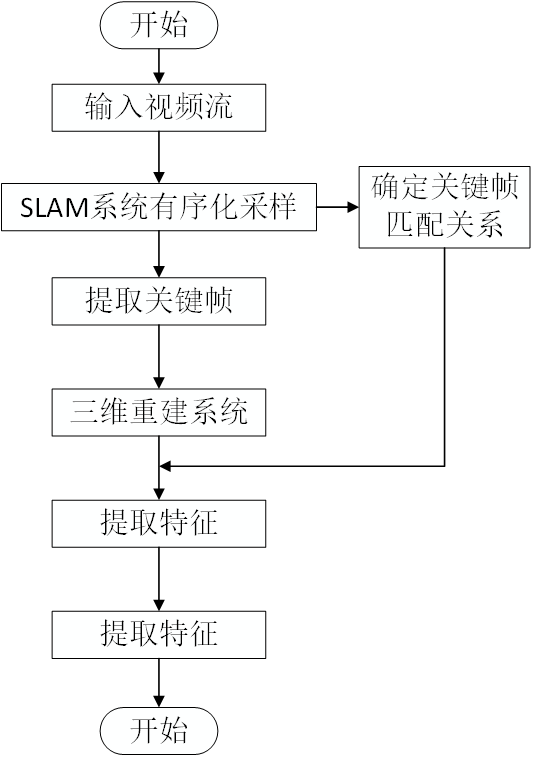
\includegraphics[height=12cm]{3Dconstr_SLAM_pipeline.png}
  \caption{融合SLAM结果的三维重建流程图}
  \label{fig:3Dconstr_SLAM_pipeline}
\end{figure}
本文将说明SLAM中关键帧的提取策略和关键帧之间的匹配策略。首先关键帧相当于SLAM的框架,是在局部一系列普通帧中选出一帧作为局部帧
的代表,记录局部信息,但相机在场景中的某个区域内固定不动时,普通帧的集合还是会不断增减,但是关键帧集合期望其不会增加。SLAM过
程中的三角化需要一定程度的共视区域才能发挥作用,所以连续的两个普通帧之间都会存在大量的信息冗余,如果所有普通帧全部参与计算,
就会极大的浪费算力和内存,因此为了保证整个SLAM系统的良好运行,都会选择关键帧来作为优化对象。此外,关键帧选择时还会对图片质量、特征点质量等进行考察,一定程度上也发挥了滤波的作用,防止无用的或错误的信息进入优化过程而破坏定位建图的准确性。
选择关键帧主要从关键帧自身和关键帧与其他关键帧的关系两个方面来考虑。一方面,关键帧自身质量要好,例如不能是非常模糊的图像、
特征点数量要充足、特征点分布要尽量均匀等等;另一方面,关键帧与其他关键帧之间的关系,需要和局部地图中的其他关键帧有少量的共
视关系,但大部分特征点是新特征点,以达到既存在约束,又尽量少的信息冗余的效果,例如局部地图点投影到此帧的点数低于一个阈值或
前一个关键帧的特征点在此帧里已经有90$\%$观测不到等等。对于关键帧的选择,一般有以下策略:

1)	距离上一关键帧的帧数是否足够多,主要从间隔的时间上来考虑,例如可以直接间隔固定帧数选择一个关键帧,这样操作流程简单,但是
整体取帧效果不好,因为对于一些运动缓慢的场景,会选择大量相似的关键帧,再次造成冗余的情况,在运动较快的场景,又容易造成大量有
效帧的缺失。

2)	距离上一关键帧的距离是否足够远,主要从空间位置上来考虑,在SLAM运行的过程中,可以根据相机位姿得到帧和帧之间的位置关系,如
果运动的距离足够大,那么可以直接将其确定为下一个关键帧,但在对某一个场景进行重复来回运动时,就会收集大量重复的关键帧。

3)	跟踪质量,主要从共视特征点上来考虑,在SLAM的过程中会记录下当前视角中的信息,一旦检测到离开当前视角则加入新的关键帧,和上
两种方法相比较能够更有效的获取到关键帧。

对于本文中三维重建图像输入的选择,优先选择第三种关键帧提取方案,避免了提取帧率过小,而丢失一些三维重建时关键的帧,提取帧率过大
而造成图片集合存在大量冗余的问题。此外通过SLAM的筛选策略也可以提前过滤掉存在运动模糊和质量过低的图像。
\subsection{增加精确性方案}
\label{sec:3.3.3}
针对~\ref{sec:3.2.3}节所提出的问题,本文提出一种结合SLAM结果的三维重建方法,以提高点云结果的鲁棒性和准确性。本文所提出的建
图过分为两个阶段:在线SLAM阶段和离线3D重建阶段。

在线SLAM系统实时获取单目相机的图像信息,结合SLAM技术快速建立scene graph及点云环境地图。由于在线SLAM注重实时性能,只是对局
部窗口进行增量优化,即使在闭环时也只进行轨迹和部分点云优化。因此所建立的scene graph及点云环境地图的精度较低。随着时间的推移
不可避免的会出现误差累计,导致闭环处出现轨迹和环境地图的断口问题。

离线3D重建阶段首先基于在线SLAM阶段所建立的粗糙scene graph及点云环境地图,以大尺度地图及运动轨迹为优化目标,利用高性能计算机的快速
处理能力进行全局优化,得到更加精确的全局稀疏地图和运动轨迹;然后基于MVS(Multi View Stereo)技术建立稠密/半稠密环境地图,
并关联深度学习所检测的语义地标及其各种属性,在半稠密环境地图中抽象出矢量语义地图。下面分别详细介绍在线SLAM过程和离线3D重建
过程。
\subsubsection{在线SLAM阶段}
\label{sec:3.3.3.1}
本文所提出的SLAM系统整体框架如图~\ref{fig:3d_constr_online_SLAM.png}所示。系统的输入为单目相机(内参标定结果已知)。SLAM
系统有前端-后端两个部分构成,前端进行特征提取及数据关联,后端进行图模型建模及Maximum a Posteriori优化。
\begin{figure}[H] % use float package if you want it here
  \centering
  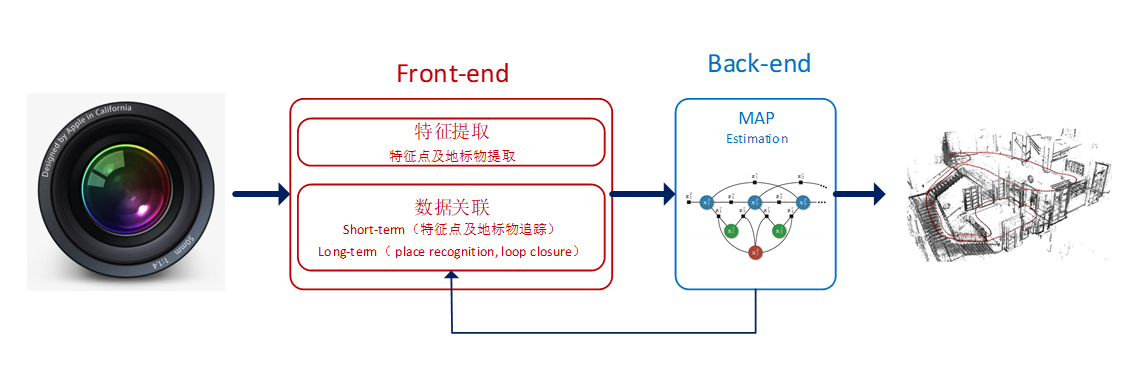
\includegraphics[height=5cm]{3d_constr_online_SLAM.png}
  \caption{前视SLAM整体框架}
  \label{fig:3d_constr_online_SLAM.png}
\end{figure}
当前主流vSLAM通过多线程技术维护3个模块(Tracking, Local Mapping and Loop Closure),实现前端-后端的各项功能,
如图~\ref{fig:3d_constr_SLAM}所示。系统以地图数据为核心,以BA(Bundle Adjustment)图模型优化为手段,实现了相机追踪、地图维护、
闭环优化。
\begin{figure}[H] % use float package if you want it here
  \centering
  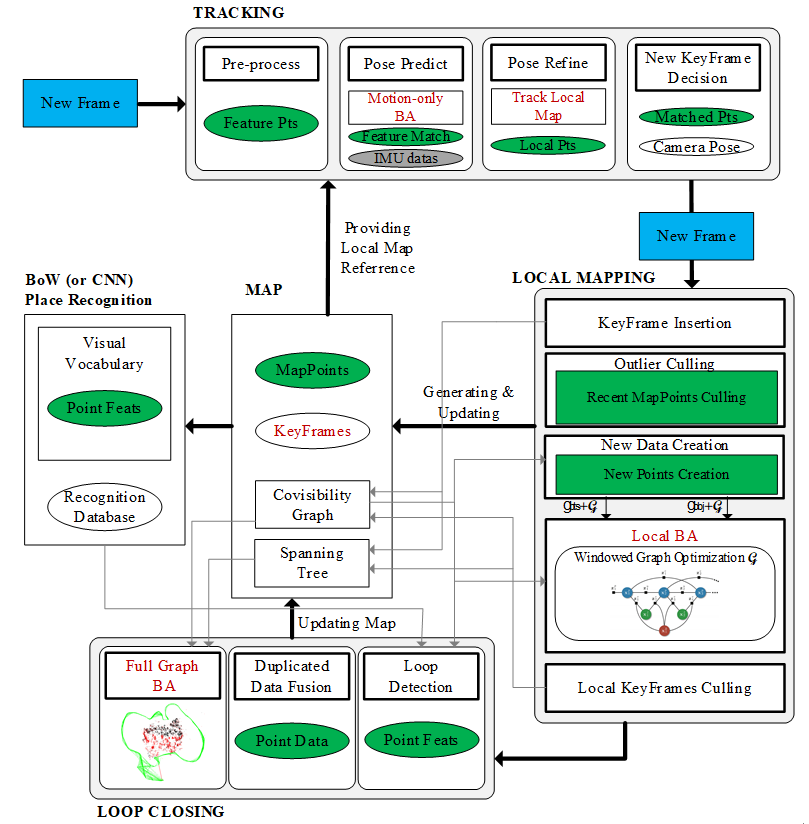
\includegraphics[height=11cm]{3d_constr_SLAM.png}
  \caption{SLAM系统框架图}
  \label{fig:3d_constr_SLAM}
\end{figure}
图中绿色模块代表传统点特征数据,通过特征提取、数据关联、地图维护、词袋维护,闭环检测等流程被不断的加入到
factor graph中并进行优化估计。
\textbf{追踪(Tracking):}模块主要负责计算相机在这两帧之间的相对运动,通过相机姿态累计得到相机的运动轨迹。首先通过图像预处
理提取点特征及语义地标特征,基于两帧间特征匹配利用Motion-only BA进行运动姿态估计,基于图像特征与地图数据关联结果利用
Track Local Map进行姿态优化,最后通过计算当前帧的信息增量的多少判别其如果是关键帧则将其输送给地图构建模块。

\textbf{地图构建(Local Mapping):}模块将追踪模块新输送过来的关键帧数据与已有关键帧数据根据可共视性约束进行数据匹配,
在factor graph图模型中加入新的点特征节点并完成数据关联,根据可共视性约束确定局部优化范围,通过Local Mapping BA建立并优
化地图数据。

\textbf{闭环(Loop Closing):}模块通过检测匹配环境地标以判断相机是否再次运动到之前曾经到过的区域,并根据这一信息对相机的运
动轨迹及地图数据进行全局修正,降低累积误差。本项目拟基于BoW词袋技术进行闭环检测。在Loop Correction时首先对地图中的重复点
特征进行融合,然后对Loop Graph主干网络进行Full BA,实现轨迹和地图数据的正确闭环。
\subsubsection{离线3D重建阶段}
\label{sec:3.3.3.2}
本文3D重建以提高建图精度为目标,其流程如图~\ref{fig:3d_constr_pipeline_sfm_mvs}所示。首先基于在线SLAM结果建立粗糙
Scene Graph及点云环境地图,以全局大尺度地图及运动轨迹为优化目标,使用鲁棒性更高的特征描述算子,利用高性能计算机的快速处理能
力进行Global Bundle Adjustment全局优化,得到更加精确的全局稀疏地图和运动轨迹。然后利用MVS(Multi View Stereo)技术对图像
中的高梯度变化区域建立半稠密环境地图。利用MVS进行半稠密建图首先提取关键帧中的边沿特征,基于SfM优化过的可共视图模型利用
triangulation计算融合边沿特征的深度信息。 
\begin{figure}[H] % use float package if you want it here
  \centering
  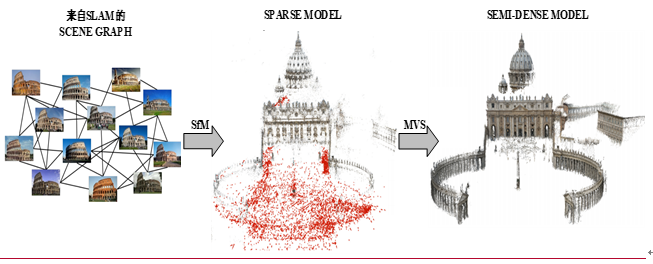
\includegraphics[height=6cm]{3d_constr_pipeline_sfm_mvs.png}
  \caption{离线3D重建技术流程图}
  \label{fig:3d_constr_pipeline_sfm_mvs}
\end{figure}
\section{本章小结}
\label{sec:3.4}
本章研究基于传统三维重建的改进方法,简述传统视觉三维重建的一般过程,分析了各个过程中的数学描述以及实现原理,
分析三维重建所存在的问题以及对应原因,包括无序图像输入的匹配耗时问题,以及对于特定场景下无法生成稳定点云的问题,
针对每种问题提出改进和提升方式,结合SLAM生成KeyFrame DataBase增强三维重建生成点云结果。
\chapter{基于纯视觉的堆体体积测量方法研究}
\label{cha:chap4}
\section{引言}
\label{sec:4.1}
利用三维重建的技术流程,可以通过输入二维图片序列的方式获取到场景中的三维稀疏点云或者稠密点云,以视觉的方式来表达场景中的信息。
虽然这些点云可以描绘出空间中的信息,但是还存在以下两个这些问题需要解决:

1)	在三维重建的过程中,由于点云坐标系都是以第一帧的相机为参考坐标系,因此点云坐标系和真实世界坐标系无法对应,对于很多实际应
用场景,都需要获取到该场景的实际水平面,来进行下一步的导航和定位;

2)	由于是单目相机,无法获取特征点的深度信息,因此对于构建出的三维重建点云没有一个绝对尺度的概念。

在解决上述两个问题的基础上,可以对空间中的封闭物体进行高度,面积或者体积的测算,对比传统方法中用激光雷达等设备来测算体积的方
式,现在就可以通过单个摄像头以纯视觉的方式来完成上述过程,并获取到一个精确的结果。本章将以三维重建的点云结果为基础,为了解决
点云的尺度问题,以及求解三维点云的水平面方程,本文将在场景中引入Aruco二维码,因为Aruco二维码本身携带尺度信息,每一种二维码
都有唯一的ID值,并且其还具备较为容易检出的角点坐标。在获取到尺度和水平面方程后,随后结合点云信息可以再进一步计算三维场景的体
积,具体流程如图~\ref{fig:getVolume}所示。

\begin{figure}[H] % use float package if you want it here
    \centering
    \includegraphics[height=5cm]{getVolume.png}
    \caption{体积测算流程图}
    \label{fig:getVolume}
  \end{figure}

\section{堆体水平面方程解析方法}
\label{sec:4.2}
对于大尺度的场景,都需要得到该场景的水平面所在的平面的方程,由于物体的遮挡,水平面很难直接通过视觉的方法构建出来,从而
导致整个场景非闭合,因此添加水平面后可以使得整个场景封闭;因此,水平面的存在能够更好的计算场景的几何特性,例如场景的高度,
面积,体积等。由于三维重建本身的点云结果都是基于参考坐标系,没有和世界坐标系对齐,本文考虑到可以结合点云中能够获取到世界坐标
系的Aruco二维码作为媒介,进行坐标系的转换,该类型二维码如图~\ref{fig:getVolume_Aruco}所示。
\begin{figure}[H] % use float package if you want it here
  \centering
  \includegraphics[height=6cm]{getVolume_Aruco.png}
  \caption{多种Aruco示意图}
  \label{fig:getVolume_Aruco}
  \end{figure}
\subsection{2D点坐标检测}
\label{sec:4.2.1}
如图~\ref{fig:getVolume_Aruco_detect}所示,可以利用二维码检测算法检测出场景中二维码的ID值,位置,大小,角点坐标等信息,因为在场景中,
Aruco二维码的布置都会有下侧两个角点直接落在水平面上,因此可以认为所有二维码的下侧角点所构成的平面即是场景的水平面。那么接下
来即可将水平面的求解转化为二维码角点所在平面的求解。在检测的过程中,需要将所有2D图片的索引和角点的位置记录下即可。

\begin{figure}[H] % use float package if you want it here
\centering
\includegraphics[height=8cm]{getVolume_Aruco_detect_1.png}
\caption{Aruco二维码检测示意图}
\label{fig:getVolume_Aruco_detect}
\end{figure}

\subsection{空间3D点映射方法}
\label{sec:4.2.2}
在上一小结中,可以获得连续视频帧中每一帧的Aruco二维码下侧两个角点的坐标值,同样的,可以直接将这些包含二维码的视频帧序列作为
三维重建的输入以获取场景的点云,考虑到Aruco的角点被作为特征点时极易被检出,因此只需要通过稀疏点云,即可获取角点在二维图像中
的坐标和三维重建点云中的三维坐标之间的对应关系。

在三维重建的过程中,可以获取到每一帧图像中所有特征点所对应的三维重建点云中的三维坐标,无论是稠密点云或者稀疏点云,都可以得到
一个对应关系,但是考虑到遍历的效率问题,则选择稀疏点云中的点击作为遍历对象。在寻找对应关系的实际过程中,会遇到二维坐标无法映
射到三维坐标点的情况,那么则会优先选择距离二维点坐标欧氏距离最近的点作为替代对象。此外,还需要注意的是,若所布置的Aruco二维
码的所有下侧点都位于同一条直线上,那么这样就无法获取准确的水平面方程,因为经过同一直线的平面并不唯一,因此在布置坐标的过程中
需要注意将所有Aruco二维码尽可能对立放置。
\subsection{平面方程解析方法}
根据上述两个步骤,可以将待求的水平面方程问题转化成求解N个三维点所在水平面方程的非线性优化问题。本文选择谷歌开源的Ceres solver
库作为解决该非线性问题的工具,Ceres可以解决边界约束鲁棒非线性最小二乘法优化的问题,表达式如下
\begin{equation}
\begin{array}{l}\underset x{min}\;\;\frac12\sum\rho_i(\parallel f_i(x_{i_1},...,x_{i_k})\parallel^2)
\\s.t.\;\;l_j\leq x_j\leq u_j\\\end{array}
\end{equation}
其中$rho_i(\parallel f_i(x_{i_1},...,x_{i_k})\parallel^2$这一部分为残差块, $f_i(.)$为代价函数,代价函数的求解依赖于一系列
参数$[x_{i_1},...,x_{i_k}]$,所有参数构成参数块,限制边界分别为$l_j$,$u_j$。$rho_i$为损失函数,其作用是减少异常值对优化结果的影响。
在利用Ceres解决非线性问题时,通常分为以下三个步骤:\\
1.	构建代价函数,也就是具体问题所对应的目标式,本小结具体解决N个三维点所在水平面的方程;\\
2.	通过代价函数构建待求解的优化问题;\\
3.	配置求解器参数并求解问题,在这一过程中主要是设定求解方程的方式。\\
上述步骤如代码~\ref{code:chap3:get_plane}所示。
\begin{lstlisting}[
  language=C++,
  numbers=left,                
  numberstyle=\footnotesize,
  frame=single,     
  basicstyle=\small\tt,    
  escapeinside = '',
  caption={获取平面方程参数的~C++~实现},
  label={code:chap3:get_plane}]
  vector<vector<float>> plane_data1;
  vector<float> planex_data1 ,planey_data1, planez_data1;'//待优化量'
  '// 第一部分:构建代价函数模型'
  struct CURVE_FITTING_COST_plane
  {
    CURVE_FITTING_COST_plane (double x,double y,double z)
    :_x( x ), _y ( y ), _z ( z ) {}
    '// 残差的计算'
    template <typename T>
    bool operator() (
      const T* const plane,    
      T* residual ) const 
    {
      residual[0] = plane[0]*T(_x) + plane[1]*T(_y) 
                  + plane[2]*T(_z) + plane[3]; 
      return true;
    }
    const double _x, _y, _z;
  };

  int main ( int argc, char** argv )
  {   
    double plane[4] = {0.1,0.1,0.2,0};
    '// 第二部分:构建最小二乘问题'
    ceres::Problem problem2;
    for ( int i=0; i<planex_data1.size(); i++ ){
      problem2.AddResidualBlock 
      (new ceres::AutoDiffFunction<CURVE_FITTING_COST_plane,1,4> 
      (new CURVE_FITTING_COST_plane 
      (planex_data1[i], planey_data1[i],planez_data1[i])),
      nullptr,
      plane);
    }
    '// 第三部分:配置求解器'
    ceres::Solver::Options options2;    
    options2.linear_solver_type = ceres::DENSE_QR;
    options2.minimizer_progress_to_stdout = true; 
    ceres::Solver::Summary summary2;                 
    ceres::Solve ( options2, &problem2, &summary2 );
    for ( auto a:plane ) {
      outfile_kabc<<a*1/plane[3]<<endl;
      }
    return 0;
  }
\end{lstlisting}
对于任意平面方程,都可以利用以下方程通过确定4个参数的方式来确定唯一解析解。
\begin{equation}Ax+By+Cz+D= 0\label{equ:plane}\end{equation}
在迭代的过程中,同时需要确定每个带估计参数的初始值,最终可以得到方程的四个参数a,b,c,d。

\section{堆体尺度估计方法}
\label{sec:4.3}
由单目视觉重建出来的点云地图都存在没有一个确定尺度的问题,地图中的特征点坐标和相机的位姿都是相对尺度,即最常见的采
取初始化成功后的前两帧作为单位尺度,后续的所有关键帧都以此为参考确定尺度。这样的做法可以获取到地图中所有描述的绝
对尺度,但无法计算出实际尺度,本文提出两种估计尺度大小的方法,这两种方法都主要是通过在场景中引入已知尺度的二维码
来确定所构点云地图的真实尺度,主要针对同一场景,通过计算两种SLAM的相机位姿或者两种SLAM中地图点坐标来确定相对尺度
和绝对尺度之间的比例,从而确定绝对尺度。流程图如图~\ref{fig:getVolume_getK}所示。
\begin{figure}[H] % use float package if you want it here
  \centering
  \includegraphics[height=12cm]{getVolume_getK.png}
  \caption{估计尺度流程图}
  \label{fig:getVolume_getK}
\end{figure}
\subsection{位姿法解算尺度}
首先,获取绝对尺度的数据,由图~\ref{fig:getVolume_Aruco_detect}所示同时可以得到相机在某一个确定的Aruco下的位姿,因为二维
码自带确定的边长信息,因此可以得到带有绝对尺度的相机位姿($T_x$,$T_y$,$T_z$)。在实际的工程中需要注意,必须选择不同状态的
相机在同一二维码下的位姿,则可以通过多个图像序列获取到多个不同位姿。

其次,再获取同一批图像序列的相对尺度,通过三维重建的结果,就可以得到每一帧相机在参考坐标系下的位姿($T_x$,$T_y$,$T_z$),
该位姿为相对尺度,因为只需要考虑到尺度的大小关系,因为不需要讨论不同坐标系之间的相对转化问题。

以上可以获取到多个针对同一场景的两种SLAM相机位姿估计结果,接下提出通过位姿来估计尺度的方法因为两种SLAM方法估计出
的相机位姿是基于不同的坐标系得到的,本文提出利用相机在不同坐标系下移动的欧式距离之间的比例来确定尺度,简化公式为:
\begin{equation}K\;=\;\frac{\triangle Pose_{rel}}{\triangle Pose_{abs}}  
\label{equ:getVolume_K}\end{equation}
同4.2.1节,利用Ceres库得到最优解K值,计算如代码~\ref{code:chap3:get_k}所示,
\begin{lstlisting}[
  language=C++,
  numbers=left,                
  numberstyle=\footnotesize,
  frame=single,     
  basicstyle=\small\tt,    
  escapeinside = '',
  caption={获取尺度值的~C++~实现},
  label={code:chap3:get_k}]
  vector<vector<float>> colmap, opencv;
  vector<float> colmap_data1 ,opencv_data1;'//待优化量'
  '// 第一部分:构建代价函数模型'
  struct CURVE_FITTING_COST_k
  {
    CURVE_FITTING_COST_k (double x,double y)
    '// 残差的计算'
    template <typename T>
    bool operator() (
      const T* const k,     
      T* residual ) const     
    {
      residual[0] = T ( _y ) - ( k[0]*T ( _x ) ); // y-ax
      return true;
    }
    const double _x, _y;
  };
  int main ( int argc, char** argv )
  {   
    double k[1] = {0};
    '// 第二部分:构建最小二乘问题'
    ceres::Problem problem;
    for ( int i=0; i<colmap_data1.size(); i++ ){
      problem.AddResidualBlock 
      (new ceres::AutoDiffCostFunction<CURVE_FITTING_COST_k, 1, 1>
      (new CURVE_FITTING_COST_k 
      (opencv_data1[i], colmap_data1[i])),
      nullptr,
      k);
    }
    '// 第三部分:配置求解器'
    ceres::Solver::Options options;   
    options.linear_solver_type = ceres::DENSE_QR;  
    options.minimizer_progress_to_stdout = true;  
    ceres::Solver::Summary summary;              
    ceres::Solve ( options, &problem, &summary );  
    for ( auto a:k ) {
      outfile_kabc<<a<<endl;
      }
  return 0;
  }
\end{lstlisting}
只需要杰出唯一参数K即可,在计算的过程中需要随机获取任意两帧之间的位姿,以减小误差。
\subsection{空间坐标点解算尺度}
对于尺度的估计,可以通过场景中已知点之间的距离通过投影获得点云之中点的实际坐标,但是空间中的已知点难以确定,而且也不易保持固定
不变,符合以上规则的点的数量又较少。因此考虑到场景中二维码标记的角点为研究对象,可以通过SLAM求得每一个二维码在图像中的位置以及
四个角点的位置,因为角点极易识别,且任意两个角点之间的实际空间距离都能够简易测量得到。

通过上一章三维重建的流程,可以获取到每一个点在二维图像中和三维空间点之间的对应关系,如图所示~\ref{fig:getVolume_get_sizebyPoint}
表示的是同一个点在二维和三维之间的对应。因为图像中的任意两个二维码角点之间的距离都是已知的,那么也可以得到三维坐标中任意两个角
点之间的绝对尺度,将这一尺度因子应用到整个地图中进行缩放,即可获得一个带有真实尺度的地图。
\begin{figure}[H] % use float package if you want it here
  \centering
  \includegraphics[height=8cm]{getVolume_get_sizebyPoint.png}
  \caption{根据空间点估计尺度流程图}
  \label{fig:getVolume_get_sizebyPoint}
\end{figure}
\section{纯视觉体积测量方法}
\label{sec:4.4}
根据以上两节可以获取到三维重建后点云的水平面和比例尺度,再此基础上计算出物体的实际体积,本文提出一种计算点云实际体积的方法,
具体流程如下:\\
1.	将所有点云结果投影在水平面上,根据场景的实际空间约束和过滤方法提出得到点云中的有效3D点集;\\
2.	通过空间变换,将三维空间点转化为水平面上的点2D点集;\\
3.	对所有点集求Delauncy三角形,计算每个三角形对应的水平高度,得到三棱柱体积;\\
4.	剔除异常三棱柱,将所有有效的三棱柱积分求和得到总体积。
流程图如图~\ref{fig:getVolume_pipeline}所示。
\begin{figure}[H] % use float package if you want it here
  \centering
  \includegraphics[height=12cm]{getVolume_pipeline.png}
  \caption{解算体积流程图}
  \label{fig:getVolume_pipeline}
\end{figure}
\subsection{有效3D点集获取}
\label{sec:4.4.1}
通过第~\ref{cha:chap3}章的方法,可以对场景获取到三维稀疏点云和稠密点云,在生成点云的过程中会把部分非感兴趣区域的内容和一些
离散的误差噪音点添加至点云结果中。针对这两种情况,本文分别提出以下对应的解决方法:\\
1.	针对非感兴趣区域,本文通过三维空间平面方程对非感兴趣区域直接进行切割剔除;\\
2.	针对随机误差噪音点,本文通过离群点检测算法进行剔除。

对于方案1,在三维重建后的点云中,只需要收集感兴趣区域内的3D点集,如图~\ref{fig:getVolume_interesting}所示,只有红色框图
内区域是感兴趣区域,可以通过上一节求出的水平面方程和二维码的底边点坐标共同约束求出空间切面方程对场景进行切割。
\begin{figure}[H] % use float package if you want it here
  \centering
  \includegraphics[height=5cm]{getVolume_interesting.png}
  \caption{三维重建感兴趣区域示意图}
  \label{fig:getVolume_interesting}
\end{figure}
对于方案2,本文采用统计滤波器即为对每个点的邻域进行一个统计分析,并修剪掉一些不符合标准的点,具体方法为在输入数据中对点到临
近点的距离分布的计算,对每一个点,计算它到所有临近点的平均距离(假设得到的结果是一个高斯分布,其形状是由均值和标准差决定),
那么平均距离在标准范围之外的点,可以被定义为离群点并从数据中去除。采用统计滤波对点云中的离散点进行滤波对比如
图~\ref{fig:getVolume_3dconstr_filter}所示。
\begin{figure}[H]
  \centering
    \subcaptionbox{对点云统计滤波前}{\label{fig:chap1:getVolume_3dconstr_noise}
    \includegraphics[width=9cm]{getVolume_3dconstr_noise.png}}
  \vskip0.5cm
    \subcaptionbox{对点云统计滤波后}{\label{fig:chap1:getVolume_3dconstr_nonoise}
    \includegraphics[width=9cm]{getVolume_3dconstr_nonoise.png}}
  \caption{点云统计滤波前后效果对比示意图}\label{fig:getVolume_3dconstr_filter}
\end{figure}

通过上一步骤,可以求出有效的3D点集,接下来需要将所有三维点云投影至二维平面上获取2D点集,简略步骤如下:\\
1.	通过~\ref{sec:4.2}节获取点云水平面和参考坐标系中的xy平面方程的法向量分别为U(A,B,C)和V(0,0,1);\\
2.	将所有的3D点集O($x_o$,$y_o$,$z_o$)根据以下公式投影水平面上,获取新的3D点集P($x_p$,$y_p$,$z_p$);
\begin{equation}
  \begin{split}
  x_p=\frac{(B^2+C^2)x_o-A(By_o+Cz_o+D)}{A^2+B^2+C^2}\\
  y_p=\frac{(A^2+C^2)y_o-B(Ax_o+Cz_o+D)}{A^2+B^2+C^2}\\
  z_p=\frac{(A^2+B^2)z_o-C(Ax_o+By_o+D)}{A^2+B^2+C^2}
  \label{equ:pxyz}
  \end{split}
\end{equation}
同时也可以根据公式计算出每一个三维空间点到水平面的方程的距离
\begin{equation}
d\;=\frac{\left|Ax_0+By_0+Cz_0+D\right|}{\sqrt{A^2+B^2+C^2}}
\end{equation}
3.	计算旋转角度:
\begin{equation}
\theta=arc\cos(\frac{P\cdot Q}{\left|P\right|\left|Q\right|})
\end{equation}
4.	计算旋转轴:在计算旋转角时可知,旋转角所在的平面为有P和Q所构成的平面,那么旋转轴必垂直该平面。
假定旋转前向量为a($a_1$, $a_2$, $a_3$), 旋转后向量为b($b_1$, $b_2$, $b_3$)。由叉乘定义得旋转轴c($c_1$, $c_2$, $c_3$)为
\begin{equation}
\begin{pmatrix}c_1\\c_2\\c_3\end{pmatrix}=\begin{pmatrix}a_2b_3-a_3b_2\\a_3b_1-a_1b_3\\a_1b_2-a_2b_1\end{pmatrix}
\end{equation}
5.	根据罗德里格旋转公式将旋转角,旋转轴的表达转化为旋转矩阵R;\\
6.	将3D点集P($x_p$,$y_p$,$z_p$)右乘上述旋转矩阵R可以得到一系列在同一平面上(所有转变后的点z值都相同)的3D点集,提取所有
3D点的x,y值构成2D点集p($x$,$y$)。
\subsection{Delaunay三角网}
\label{sec:4.4.3}
通过~\ref{sec:4.2}小结,可以得到在由在同一平面上的3D点集转化成的2D点集和每一个2D点集对应的距离值d。在本节中将对2D点集进行
三角剖分,获得Dealunay三角网,Delaunay三角网是一系列相连的但不重叠的三角形的集合, 而且这些三角形的外接圆不包含这个面域的其
他任何点,如图~\ref{fig:getVolume_Delaunay}所示。
\begin{figure}[H] % use float package if you want it here
  \centering
  \includegraphics[height=6cm]{getVolume_Delaunay.png}
  \caption{Delaunay三角网示意图}
  \label{fig:getVolume_Delaunay}
\end{figure}
获取Delaunay三角网格的一般步骤为:\\
1.	构造一个超级三角形,包含所有散点,放入三角形链表;\\
2.	将点集中的散点依次插入,在三角形链表中找出其外接圆包含插入点的三角形(称为该点的影响三角形),删除影响三角形的公共边,
将插入点同影响三角形的全部顶点连接起来,从而完成一个点在Delaunay三角形链表中的插入;\\
3.	根据优化准则对局部新形成的三角形进行优化。将形成的三角形放入Delaunay三角形链表;\\
4.	循环执行上述第2步,直到所有散点插入完毕。\\
由于Delaunay剖分具备具备最接近(以最近的三点形成三角形,且各线段(三角形的边)皆不相交)和区域性(新增、删除、移动某一个顶点
时只会影响临近的三角形)的特性,可以对点集所构成的平面进行拟合。通过以上流程可以获得三角形的集合以及三角形中每个顶点对应的距
离,取三个顶点距离的平均值作为三棱柱的高,每个三角形的面积按照公式~\ref{equ:tri_s}计算,即可获得所有三棱柱的体积。
\begin{equation}
S_\bigtriangleup=\frac12\times\left(x_1y_2-x_1y_3+x_2y_3-x_2y_1+x_3y_1-x_2y_2\right)\label{equ:tri_s}
\end{equation}
\subsection{积分三棱柱}
\label{sec:4.4.4}
通过以上步骤,可以将三维重建后点云体积的求解转化成对多个三棱柱积分的求解,因为所有三棱柱的体积值都分布在某一个区间内(并不完
全服从正太分布),对于部分偏差较大的三棱柱体积值应该通过算法进行剔除。本文采用箱形图的方法来处理这一问题,箱形图不受异常值的
影响,能够准确稳定地描绘出数据的离散分布情况,同时也利于数据的清洗。
\begin{figure}[H] % use float package if you want it here
  \centering
  \includegraphics[height=6cm]{getVolume_boxplot.png}
  \caption{Delaunay三角网示意图}
  \label{fig:getVolume_boxplot}
\end{figure}
箱形图如图~\ref{fig:getVolume_boxplot}所示,主要需要求解出数据中的5个特征数据值,包
括下四分位数Q1,上四分位数Q3,四分位距IQR=Q3-Q1,以及上限Q3+1.5IQR和下限Q1-1.5IQR,对于上下限之外的内容需要剔除,最终结
合\label{sec:4.3}所估算出的尺度,以及所有有效三棱柱的体积按照公式~\ref{equ:get_volume}即可估计出物体中感兴趣区域的实际
体积值。
\begin{equation}
  V\;=K^3\;\ast\sum_i\frac13\ast S_\bigtriangleup\times\sum_{j=1}^3d_j\label{equ:get_volume}
\end{equation}
\section{本章小结}
本章的主要目的是通过纯视觉的方式对点云体积进行测量,以获取到堆体的实际体积。

本章提出了通过纯视觉方法进行堆体体积测量的一般步骤,通过位姿比例或空间三维点坐标比例估计出堆体点云和堆体实际空间点之间的尺度关系;通过2D角点获取对应3D映射点,通过非线性优化求解水平面方程参数的最优值;最后再结合水平面投影求解Delaunay三角形,积分三棱柱以估计出堆体点云的体积。

本章所提出方法完全基于视觉方案,整体流程可自动化完成,且可以在相似场景中复用。






% \chapter{视觉定位与三维体积测试与分析}
\label{cha:chap5}
\section{引言}
\label{sec:5.1}
做实验做实验做实验
\section{视觉定位系统测试}
\label{sec:5.2}
\subsection{视觉定位系统实验步骤设计}
\label{sec:5.2.1}
在第二章,本文提出了一种结合二维码的SLAM视觉系统,利用该系统可以估计出带有真实尺度的相机位姿,以及能够得到真实世界坐标系下的
相机位置。本次实验主要利用上述方法在复杂封闭,且无GPS信号的环境下,结合二维码视觉标签进行无人机定位,通过获得到的位置信息信
息进行下一步的飞行控制。本次实验的准备过程主要分为三个步骤,布置场景,生成地图,无人机自主循迹。

首先是场景布置,选择在空旷场地中,布置二维码视觉标签,保证每个二维码的尺度大小完全一致,且二维码之间尽可能等间距布置,场景中的
二维码ID完全独立不同,设计图和实际布置图分别如图~\ref{fig:scene_imagine}和图~\ref{fig:scene_reality}所示。在本次实验中,所原选择的二维码实际大小为0.73m,相邻二维码之间的距
离为4m,整个实验区域面积为400m2(20m*20m)。

\begin{figure}[H] % use float package if you want it here
  \centering
  \includegraphics[height=8cm]{scene_imagine.png}
  \caption{实验场景设计示意图}
  \label{fig:scene_imagine}
\end{figure}
\begin{figure}[H] % use float package if you want it here
  \centering
  \includegraphics[height=8cm]{scene_reality.png}
  \caption{实验场景真实布置图}
  \label{fig:scene_reality}
\end{figure}

在布置好场景后,需要根据实际场景生成地图信息。当无人机首次在无先验地图的环境下飞行时,需要人工手动控制,完成无人机的飞行和地图
生成工作,在无人机的手动飞行过程中,其飞行区域需要尽可能覆盖所有场景以确保生产完整的地图,根据实际场景生成的地图如图~\ref{fig:map_generator}
所示,其中正方形框代表二维码,蓝色相机表示代表视觉定位产生的关键帧,点代表地图中的特征点。

\begin{figure}[H] % use float package if you want it here
  \centering
  \includegraphics[height=8cm]{map_generator.png}
  \caption{视觉算法生成地图}
  \label{fig:map_generator}
\end{figure}

当获取到完整的地图信息地图后,可以让无人机按照认为规定的轨迹进行自动循迹飞行,首先设计如下图~\ref{fig:flight_route}所示的轨
迹图,其中起始点为ID=0的二维码处,红色箭头代表无人机的飞行轨迹,对于无人机的飞控过程,按照设定循迹点的方案来实现,即在整个轨迹
中给定多个循迹点坐标,使得无人机按照设定的坐标顺序进行飞行。
\begin{figure}[H] % use float package if you want it here
  \centering
  \includegraphics[height=8cm]{flight_route.png}
  \caption{无人机自主飞行轨迹设计图}
  \label{fig:flight_route}
\end{figure}
\subsection{视觉定位系统实验结果分析}
\label{sec:5.2.2}
按照上述实验流程让无人机进行自主飞行,可以直接获取到视觉算法生成的地图以及无人机在飞行的过程中生成的三维坐标,根据这些数据可以对
视觉算法关于无人机自主定位的效果进行定量的分析,本节主要从生成地图的精度,无人机三维坐标的精度以及轨迹精度三个方面进行定量分析。

首先对于地图精度,根据图~\ref{fig:scene_reality}生成的地图,通过对地图的解析,可以获取每一个二维码的三维位置坐标,如
表~\ref{tab:chap1:marker_pose}所示。

\begin{table}[h]
  \centering
  \caption{二维码标志位置实际测量值}
  \label{tab:chap1:marker_pose}
  \begin{tabular}{C{3.6cm}L{2.4cm}L{2.4cm}L{2.4cm}}
  \toprule
  \textbf{序号} & \textbf{X} & \textbf{Y} & \textbf{Z} \\
  \midrule
  0      & -2.63   & 	1.32 & 7 .86            \\
  3      & -14.69  & 	3.88 & 7.80            \\
  5      & -6.05 	 &  6.34 & 7.45           \\
  6      & -9.83 	 &  -9.83 & 7.45           \\
  9      & -5.13 	 &  10.44 & 7.30           \\
  10     & -9.17   &	11.22 &	7.24        \\
  12     & -0.33 	 &  13.56 & 7.34 	             \\
  15     & -12.25  & 	16.15 &	7.27            \\
  \bottomrule
  \end{tabular}
\end{table}

针对地图的精度,可以提出以下两个判断指标。\\
1)任意两个二维码之间距离的测量值和理论值的误差比较;\\
2)所有二维码是否在同一个坐标平面。

针对指标1,计算得到表~\ref{tab:chap1:marker_map_error},经过计算得到地图中二维码的误差精度为3.1$\%$。

\begin{table}[h]
    \centering
    \caption{二维码位置误差}
    \label{tab:chap1:marker_map_error}
    \begin{tabular}{C{1.6cm}C{1.6cm}C{2.4cm}C{2.4cm}C{3.2cm}}
    \toprule
    \textbf{ID1} & \textbf{ID2} & \textbf{实际值} & \textbf{理论值} & \textbf{误差率} \\
    \midrule
    0&	3&	12.33&	12&	2.75 $\%$\\
    0&	5&	6.07&	5.65&	7.43$\%$\\
    0&	6&	9.26&	8.94&	3.58$\%$\\
    0&	9&	9.46&	8.94&	5.82$\%$\\
    0&	10&	11.86&11.31&	4.86$\%$\\
    0&	12&	12.45&	12&	3.75$\%$\\
    0&  15&	17.67&	16.97&	4.12$\%$\\
    3&	5&	8.99&	8.94&	0.56$\%$\\
    3&	6&	5.85&	5.65&	3.54$\%$\\
    3&	9&	11.6&	11.31&	2.56$\%$\\
    3&	10&	9.18&	8.94&	2.68$\%$\\
    3&	12&	17.32&	16.97&	2.06$\%$\\
    3&	15&	12.51&	12&	4.25$\%$\\
    5&	6&	3.87&	4&	3.25$\%$\\
    5&	9&	4.21&	4&	5.25$\%$\\
    5&	10&	5.79&	5.65&	2.48$\%$\\
    5&	12&	9.21&	8.94&	3.02$\%$\\
    5&	15&	11.61&	11.31&	2.65$\%$\\
    6&	9&	5.75&	5.65&	1.77$\%$\\
    6&	10&	4.13&	4&	3.25$\%$\\
    6&	12&	11.47&	11.31&	1.41$\%$\\
    6&	15&	9.33&	8.94&	4.36$\%$\\
    9&	10&	4.11&	4&	2.75$\%$\\
    9&	12&	5.72&	5.65&	1.24$\%$\\
    9&	15&	9.12&	8.94&	2.01$\%$\\
    10&	12&	9.15&	8.94&	2.35$\%$\\
    10&	15&	5.81&	5.65&	2.83$\%$\\
    12&	15&	12.2&	12&	1.67$\%$\\  
    \bottomrule
    \end{tabular}
\end{table}

针对指标2,绘制出每个二维码的在同一个坐标平面的误差情况,如图~\ref{fig:marker_map_error_Z}所示,,平均误差为0.18m
可以认定所有二维码基本都在同一水平面内。
\begin{figure}[H] % use float package if you want it here
  \centering
  \includegraphics[height=8cm]{marker_map_error_Z.png}
  \caption{二维码Z方向数据}
  \label{fig:marker_map_error_Z}
\end{figure}
其次对于无人机三维坐标的精度,以无人机自带GPS测距仪器测定出的坐标为真值,和视觉算法计算出来的位置信息进行对比,选择无人机
在0-800帧的数据,在X、Y、Z方向得到的结果分别如图~\ref{fig:chap2:pose_xyz}所示,其中蓝色连线为视觉算法检测出的坐标值,红色
连线无人机GPS检测出的真实值。
\begin{figure}[htbp]
  \centering
    \subcaptionbox{X方向GPS和视觉算法对比图}{\label{fig:chap1:pose_x}
    \includegraphics[width=6cm]{pose_x.png}\hskip2cm}
    \subcaptionbox{Y方向GPS和视觉算法对比图}{\label{fig:chap1:pose_y}
    \includegraphics[width=6cm]{pose_y.png}}
  \vskip0.5cm
    \subcaptionbox{Z方向GPS和视觉算法对比图}{\label{fig:chap1:pose_z}
    \includegraphics[width=6cm]{pose_z.png}\hskip2cm}
  \caption{各方向GPS和视觉算法对比图}\label{fig:chap2:pose_xyz}
\end{figure}
随后,计算真值和测量值之间的误差,在X、Y、Z方向分别得到结果如图~\ref{fig:chap2:pose_error_xyz}所示,对于X、Y、Z三个方向分别可以
得到距离误差为0.22m、0.37m、0.107m。
\begin{figure}[H]
    \centering
      \subcaptionbox{X方向GPS和视觉算法对比图}{\label{fig:chap1:pose_error_x}
      \includegraphics[width=12cm]{pose_error_x.png}}
    \vskip0.5cm
      \subcaptionbox{Z方向GPS和视觉算法对比图}{\label{fig:chap1:pose_error_y}
      \includegraphics[width=12cm]{pose_error_y.png}}
    \vskip0.5cm
      \subcaptionbox{Z方向GPS和视觉算法对比图}{\label{fig:chap1:pose_error_z}
      \includegraphics[width=12cm]{pose_error_z.png}}
    \caption{各方向GPS和视觉算法误差对比图}\label{fig:chap2:pose_error_xyz}
\end{figure}
最后,对无人机的轨迹精度进行对比。无人机在自主飞行过程中能够产生实时的相对于真实世界坐标系的定位信息,将其与GPS生成的定位信息
进行对比,如图~\ref{fig:pose_map}所示。
\begin{figure}[H] % use float package if you want it here
  \centering
  \includegraphics[height=10cm]{pose_map.png}
  \caption{无人机轨迹对比示意图}
  \label{fig:pose_map}
\end{figure}
对于无人机的直飞路线,误差较小,GPS和视觉算法测算出的轨迹基本吻合,但是在对于转弯改变方向的区间,两者之间的相对误差则较大,考虑
其原因为在转弯处所设计的循迹点相对比较稠密,导致在该区域内无人机需要改变的方向更大,导致视觉算法在测算时由于方法振动的缘故产生
较大的误差。
\section{三维重建系统测试}
\label{sec:5.3}
\subsection{三维重建系统实验步骤设计}
\label{sec:5.3.1}
\subsection{三维重建系统实验结果分析}
\label{sec:5.3.2}
\section{体积测算系统测试}
\label{sec:5.4}
\subsection{体积测算系统实验步骤设计}
\label{sec:5.4.1}
在第四章,本文提出了一种基于纯视觉方法来测算场景中物体体积的方法,基于对实验场景进行的三维重建结果,整个实验步骤主要包括以下四个方面\\
1)解析水平面的方程\\
2)估计出整个场景的实际尺度\\
3)点云提纯\\
4)计算三维点云的体积。
在对测算场景体积之前,需要收集该场景的连续视频帧以获取其三维重建的结果,所收集的连续视频帧序列如图~\ref{fig:getVolume_inputCamera}
所示,其三维重建的稀疏点云和稠密结果分别如图和图所示。考虑到稠密点云的点集数量过大,在遍历和查询时都会比较耗时,且稀疏点云也包含了每个特征点的坐标信息和相机的位姿信息,后续在解析水平面方程和估计场景实际尺度时选择稀疏点云作为分析对象。



\begin{figure}[H] % use float package if you want it here
  \centering
  \includegraphics[height=9cm]{getVolume_inputCamera.png}
  \caption{三维重建输入视频序列图}
  \label{fig:getVolume_inputCamera}
  \end{figure}


\subsection{体积测算系统实验结果分析}
\label{sec:5.4.2}
% \chapter{总结和展望}
\label{cha:chap6}
\section{全文总结}
\label{sec:6.1}
总结总结
\
\section{展望}
\label{sec:6.2}
展望展望

%%% 其它部分
%\backmatter

\begin{acknowledgement}
衷心感谢导师岳继光教授和董延超副教授对本人的精心指导。他们的言传身教将使
我终生受益。
\end{acknowledgement}

% 参考文献
\printTJbibliography


% 附录
% \begin{appendix}
% \chapter{外文资料原文}
\label{cha:engorg}
As one of the most widely used techniques in operations research, {\em
  mathematical programming} is defined as a means of maximizing a quantity known
as {\em objective function}, subject to a set of constraints represented by
equations and inequalities. Some known subtopics of mathematical programming are
linear programming, nonlinear programming, multiobjective programming, goal
programming, dynamic programming, and multilevel programming$^{[1]}$.

It is impossible to cover in a single chapter every concept of mathematical
programming. This chapter introduces only the basic concepts and techniques of
mathematical programming such that readers gain an understanding of them
throughout the book$^{[2,3]}$.


\section{Single-Objective Programming}
The general form of single-objective programming (SOP) is written
as follows,
\begin{equation}\tag*{(123)} % 如果附录中的公式不想让它出现在公式索引中,那就请
                             % 用 \tag*{xxxx}
\left\{\begin{array}{l}
\max \,\,f(x)\\[0.1 cm]
\mbox{subject to:} \\ [0.1 cm]
\qquad g_j(x)\le 0,\quad j=1,2,\cdots,p
\end{array}\right.
\end{equation}
which maximizes a real-valued function $f$ of
$x=(x_1,x_2,\cdots,x_n)$ subject to a set of constraints.

\newtheorem{mpdef}{Definition}[chapter]
\begin{mpdef}
In SOP, we call $x$ a decision vector, and
$x_1,x_2,\cdots,x_n$ decision variables. The function
$f$ is called the objective function. The set
\begin{equation}\tag*{(456)} % 这里同理,其它不再一一指定。
S=\left\{x\in\Re^n\bigm|g_j(x)\le 0,\,j=1,2,\cdots,p\right\}
\end{equation}
is called the feasible set. An element $x$ in $S$ is called a
feasible solution.
\end{mpdef}

\newtheorem{mpdefop}[mpdef]{Definition}
\begin{mpdefop}
A feasible solution $x^*$ is called the optimal
solution of SOP if and only if
\begin{equation}
f(x^*)\ge f(x)
\end{equation}
for any feasible solution $x$.
\end{mpdefop}

One of the outstanding contributions to mathematical programming was known as
the Kuhn-Tucker conditions\ref{eq:ktc}. In order to introduce them, let us give
some definitions. An inequality constraint $g_j(x)\le 0$ is said to be active at
a point $x^*$ if $g_j(x^*)=0$. A point $x^*$ satisfying $g_j(x^*)\le 0$ is said
to be regular if the gradient vectors $\nabla g_j(x)$ of all active constraints
are linearly independent.

Let $x^*$ be a regular point of the constraints of SOP and assume that all the
functions $f(x)$ and $g_j(x),j=1,2,\cdots,p$ are differentiable. If $x^*$ is a
local optimal solution, then there exist Lagrange multipliers
$\lambda_j,j=1,2,\cdots,p$ such that the following Kuhn-Tucker conditions hold,
\begin{equation}
\label{eq:ktc}
\left\{\begin{array}{l}
    \nabla f(x^*)-\sum\limits_{j=1}^p\lambda_j\nabla g_j(x^*)=0\\[0.3cm]
    \lambda_jg_j(x^*)=0,\quad j=1,2,\cdots,p\\[0.2cm]
    \lambda_j\ge 0,\quad j=1,2,\cdots,p.
\end{array}\right.
\end{equation}
If all the functions $f(x)$ and $g_j(x),j=1,2,\cdots,p$ are convex and
differentiable, and the point $x^*$ satisfies the Kuhn-Tucker conditions
(\ref{eq:ktc}), then it has been proved that the point $x^*$ is a global optimal
solution of SOP.

\subsection{Linear Programming}
\label{sec:lp}

If the functions $f(x),g_j(x),j=1,2,\cdots,p$ are all linear, then SOP is called
a {\em linear programming}.

The feasible set of linear is always convex. A point $x$ is called an extreme
point of convex set $S$ if $x\in S$ and $x$ cannot be expressed as a convex
combination of two points in $S$. It has been shown that the optimal solution to
linear programming corresponds to an extreme point of its feasible set provided
that the feasible set $S$ is bounded. This fact is the basis of the {\em simplex
  algorithm} which was developed by Dantzig as a very efficient method for
solving linear programming.
\begin{table}[ht]
\centering
  \centering
  \caption*{Table~1\hskip1em This is an example for manually numbered table, which
    would not appear in the list of tables}
  \label{tab:badtabular2}
  \begin{tabular}[c]{|c|m{0.8in}|c|c|c|c|c|}\hline
    \multicolumn{2}{|c|}{Network Topology} & \# of nodes &
    \multicolumn{3}{c|}{\# of clients} & Server \\\hline
    GT-ITM & Waxman Transit-Stub & 600 &
    \multirow{2}{2em}{2\%}&
    \multirow{2}{2em}{10\%}&
    \multirow{2}{2em}{50\%}&
    \multirow{2}{1.2in}{Max. Connectivity}\\\cline{1-3}
    \multicolumn{2}{|c|}{Inet-2.1} & 6000 & & & &\\\hline
    \multirow{2}{1in}{Xue} & Rui  & Ni &\multicolumn{4}{c|}{\multirow{2}*{\tongjithesis}}\\\cline{2-3}
    & \multicolumn{2}{c|}{ABCDEF} &\multicolumn{4}{c|}{} \\\hline
\end{tabular}
\end{table}

Roughly speaking, the simplex algorithm examines only the extreme points of the
feasible set, rather than all feasible points. At first, the simplex algorithm
selects an extreme point as the initial point. The successive extreme point is
selected so as to improve the objective function value. The procedure is
repeated until no improvement in objective function value can be made. The last
extreme point is the optimal solution.

\subsection{Nonlinear Programming}

If at least one of the functions $f(x),g_j(x),j=1,2,\cdots,p$ is nonlinear, then
SOP is called a {\em nonlinear programming}.

A large number of classical optimization methods have been developed to treat
special-structural nonlinear programming based on the mathematical theory
concerned with analyzing the structure of problems.
\begin{figure}[h]
  \centering
  \includegraphics[clip]{tongji-lib-logo.jpg}
  \caption*{Figure~1\hskip1em This is an example for manually numbered figure,
    which would not appear in the list of figures}
  \label{tab:badfigure2}
\end{figure}

Now we consider a nonlinear programming which is confronted solely with
maximizing a real-valued function with domain $\Re^n$.  Whether derivatives are
available or not, the usual strategy is first to select a point in $\Re^n$ which
is thought to be the most likely place where the maximum exists. If there is no
information available on which to base such a selection, a point is chosen at
random. From this first point an attempt is made to construct a sequence of
points, each of which yields an improved objective function value over its
predecessor. The next point to be added to the sequence is chosen by analyzing
the behavior of the function at the previous points. This construction continues
until some termination criterion is met. Methods based upon this strategy are
called {\em ascent methods}, which can be classified as {\em direct methods},
{\em gradient methods}, and {\em Hessian methods} according to the information
about the behavior of objective function $f$. Direct methods require only that
the function can be evaluated at each point. Gradient methods require the
evaluation of first derivatives of $f$. Hessian methods require the evaluation
of second derivatives. In fact, there is no superior method for all
problems. The efficiency of a method is very much dependent upon the objective
function.

\subsection{Integer Programming}

{\em Integer programming} is a special mathematical programming in which all of
the variables are assumed to be only integer values. When there are not only
integer variables but also conventional continuous variables, we call it {\em
  mixed integer programming}. If all the variables are assumed either 0 or 1,
then the problem is termed a {\em zero-one programming}. Although integer
programming can be solved by an {\em exhaustive enumeration} theoretically, it
is impractical to solve realistically sized integer programming problems. The
most successful algorithm so far found to solve integer programming is called
the {\em branch-and-bound enumeration} developed by Balas (1965) and Dakin
(1965). The other technique to integer programming is the {\em cutting plane
  method} developed by Gomory (1959).

\hfill\textit{Uncertain Programming\/}\quad(\textsl{BaoDing Liu, 2006.2})

\section*{References}
\noindent{\itshape NOTE: these references are only for demonstration, they are
  not real citations in the original text.}

\begin{enumerate}[{$[$}1{$]$}]
\item Donald E. Knuth. The \TeX book. Addison-Wesley, 1984. ISBN: 0-201-13448-9
\item Paul W. Abrahams, Karl Berry and Kathryn A. Hargreaves. \TeX\ for the
  Impatient. Addison-Wesley, 1990. ISBN: 0-201-51375-7
\item David Salomon. The advanced \TeX book.  New York : Springer, 1995. ISBN:0-387-94556-3
\end{enumerate}

\chapter{外文资料的调研阅读报告或书面翻译}
\section{单目标规划}
北冥有鱼,其名为鲲。鲲之大,不知其几千里也。化而为鸟,其名为鹏。鹏之背,不知其几
千里也。怒而飞,其翼若垂天之云。是鸟也,海运则将徙于南冥。南冥者,天池也。
\begin{equation}\tag*{(123)}
 p(y|\mathbf{x}) = \frac{p(\mathbf{x},y)}{p(\mathbf{x})}=
\frac{p(\mathbf{x}|y)p(y)}{p(\mathbf{x})}
\end{equation}

吾生也有涯,而知也无涯。以有涯随无涯,殆已!已而为知者,殆而已矣!为善无近名,为
恶无近刑,缘督以为经,可以保身,可以全生,可以养亲,可以尽年。

\subsection{线性规划}
庖丁为文惠君解牛,手之所触,肩之所倚,足之所履,膝之所倚,砉然响然,奏刀騞然,莫
不中音,合于桑林之舞,乃中经首之会。
\begin{table}[ht]
\centering
  \centering
  \caption*{表~1\hskip1em 这是手动编号但不出现在索引中的一个表格例子}
  \label{tab:badtabular3}
  \begin{tabular}[c]{|c|m{0.8in}|c|c|c|c|c|}\hline
    \multicolumn{2}{|c|}{Network Topology} & \# of nodes &
    \multicolumn{3}{c|}{\# of clients} & Server \\\hline
    GT-ITM & Waxman Transit-Stub & 600 &
    \multirow{2}{2em}{2\%}&
    \multirow{2}{2em}{10\%}&
    \multirow{2}{2em}{50\%}&
    \multirow{2}{1.2in}{Max. Connectivity}\\\cline{1-3}
    \multicolumn{2}{|c|}{Inet-2.1} & 6000 & & & &\\\hline
    \multirow{2}{1in}{Xue} & Rui  & Ni &\multicolumn{4}{c|}{\multirow{2}*{\tongjithesis}}\\\cline{2-3}
    & \multicolumn{2}{c|}{ABCDEF} &\multicolumn{4}{c|}{} \\\hline
\end{tabular}
\end{table}

文惠君曰:“嘻,善哉!技盖至此乎?”庖丁释刀对曰:“臣之所好者道也,进乎技矣。始臣之
解牛之时,所见无非全牛者;三年之后,未尝见全牛也;方今之时,臣以神遇而不以目视,
官知止而神欲行。依乎天理,批大郤,导大窾,因其固然。技经肯綮之未尝,而况大坬乎!
良庖岁更刀,割也;族庖月更刀,折也;今臣之刀十九年矣,所解数千牛矣,而刀刃若新发
于硎。彼节者有间而刀刃者无厚,以无厚入有间,恢恢乎其于游刃必有余地矣。是以十九年
而刀刃若新发于硎。虽然,每至于族,吾见其难为,怵然为戒,视为止,行为迟,动刀甚微,
謋然已解,如土委地。提刀而立,为之而四顾,为之踌躇满志,善刀而藏之。”

文惠君曰:“善哉!吾闻庖丁之言,得养生焉。”


\subsection{非线性规划}
孔子与柳下季为友,柳下季之弟名曰盗跖。盗跖从卒九千人,横行天下,侵暴诸侯。穴室枢
户,驱人牛马,取人妇女。贪得忘亲,不顾父母兄弟,不祭先祖。所过之邑,大国守城,小
国入保,万民苦之。孔子谓柳下季曰:“夫为人父者,必能诏其子;为人兄者,必能教其弟。
若父不能诏其子,兄不能教其弟,则无贵父子兄弟之亲矣。今先生,世之才士也,弟为盗
跖,为天下害,而弗能教也,丘窃为先生羞之。丘请为先生往说之。”
\begin{figure}[h]
  \centering
  \includegraphics{hello}
  \caption*{图~1\hskip1em 这是手动编号但不出现索引中的图片的例子}
  \label{tab:badfigure3}
\end{figure}

柳下季曰:“先生言为人父者必能诏其子,为人兄者必能教其弟,若子不听父之诏,弟不受
兄之教,虽今先生之辩,将奈之何哉?且跖之为人也,心如涌泉,意如飘风,强足以距敌,
辩足以饰非。顺其心则喜,逆其心则怒,易辱人以言。先生必无往。”

孔子不听,颜回为驭,子贡为右,往见盗跖。

\subsection{整数规划}
盗跖乃方休卒徒大山之阳,脍人肝而餔之。孔子下车而前,见谒者曰:“鲁人孔丘,闻将军
高义,敬再拜谒者。”谒者入通。盗跖闻之大怒,目如明星,发上指冠,曰:“此夫鲁国之
巧伪人孔丘非邪?为我告之:尔作言造语,妄称文、武,冠枝木之冠,带死牛之胁,多辞缪
说,不耕而食,不织而衣,摇唇鼓舌,擅生是非,以迷天下之主,使天下学士不反其本,妄
作孝弟,而侥幸于封侯富贵者也。子之罪大极重,疾走归!不然,我将以子肝益昼餔之膳。”


\chapter{其它附录}
其它附录的内容可以放到这里,当然如果你愿意,可以把这部分也放到独立的文件中,然后
将其\verb|\input| 到主文件中。
% \end{appendix}

% 个人简历
\begin{resume}
\resumeitem{个人简历:}
\noindent 1994年4月出生于河南省信阳市。\\
\noindent 2013年9月考入中南大学信息科学与工程学院自动化专业,2017年7月本科毕业并获得工学学士学位。\\
\noindent 2017年9月考入同济大学控制工程专业系攻读工学学位至今。

\resumeitem{发表论文:} % 发表的和录用的合在一起
\begin{enumerate}[{[}1{]}]
\item Yang Y, Ren T L, Zhang L T, et al. Miniature microphone with silicon-
  based ferroelectric thin films. Integrated Ferroelectrics, 2003,
  52:229-235. (SCI 收录, 检索号:758FZ.)
\item 杨轶, 张宁欣, 任天令, 等. 硅基铁电微声学器件中薄膜残余应力的研究. 中国机
  械工程, 2005, 16(14):1289-1291. (EI 收录, 检索号:0534931 2907.)
\item 杨轶, 张宁欣, 任天令, 等. 集成铁电器件中的关键工艺研究. 仪器仪表学报,
  2003, 24(S4):192-193. (EI 源刊.)
\item Yang Y, Ren T L, Zhu Y P, et al. PMUTs for handwriting recognition. In
  press. (已被 Integrated Ferroelectrics 录用. SCI 源刊.)
\item Wu X M, Yang Y, Cai J, et al. Measurements of ferroelectric MEMS
  microphones. Integrated Ferroelectrics, 2005, 69:417-429. (SCI 收录, 检索号
  :896KM.)
\item 贾泽, 杨轶, 陈兢, 等. 用于压电和电容微麦克风的体硅腐蚀相关研究. 压电与声
  光, 2006, 28(1):117-119. (EI 收录, 检索号:06129773469.)
\item 伍晓明, 杨轶, 张宁欣, 等. 基于MEMS技术的集成铁电硅微麦克风. 中国集成电路, 
  2003, 53:59-61.
\end{enumerate}

\resumeitem{研究成果:} % 有就写,没有就删除
\begin{enumerate}[{[}1{]}]
\item 任天令, 杨轶, 朱一平, 等. 硅基铁电微声学传感器畴极化区域控制和电极连接的
  方法: 中国, CN1602118A. (中国专利公开号.)
\item Ren T L, Yang Y, Zhu Y P, et al. Piezoelectric micro acoustic sensor
  based on ferroelectric materials: USA, No.11/215, 102. (美国发明专利申请号.)
\end{enumerate}

\end{resume}

\end{document}
